% !TeX spellcheck = en_US
% !TeX encoding = UTF-8
\documentclass[a4paper]{article}
\usepackage{graphics, graphicx}
\usepackage{fancyvrb, enumerate}
\usepackage{amsmath, amssymb, amscd, amsfonts}
\usepackage{geometry}
\usepackage{multirow}
\usepackage{url}
\usepackage{listings, listing}
\usepackage{color}
\usepackage{mathptmx}
\usepackage[numberedbib]{apacite}
\usepackage[style=iso]{datetime2}
\usepackage{csvsimple, booktabs}
\usepackage[maxfloats=256]{morefloats}
\maxdeadcycles=1000

\geometry
{
    top = 20mm,
    bottom = 20mm,
    left = 20mm,
    right = 20mm
}

\title{Periodontitis}
\author{
    Jaewoong Lee
    \and
    Seunghoon Kim
    \and
    Semin Lee
}
\date{\today}

\begin{document}
   	\maketitle
    \newpage

    \tableofcontents
    \listoftables
    \listoffigures
    \newpage

    \section{Introduction}
        \subsection{Microbiome}
            The microbiome is consists of microbiota, the micro-organisms that live inside and on humans \cite{microbiome1}. The microbiome is also about $10^{13}$ micro-organisms whose that collective genome \cite{microbiome2}.

            \begin{figure}[p]
                \centering
                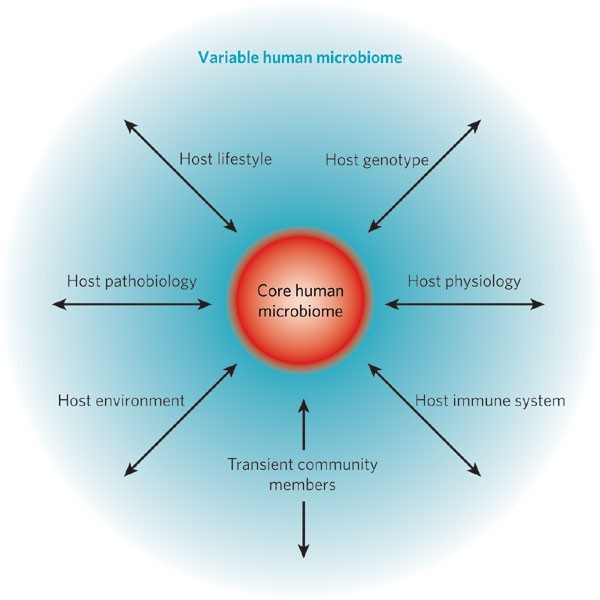
\includegraphics[width=0.5 \linewidth]{figures/microbiome.jpg}
                \caption{Concept of a Core Human Microbiome \protect\cite{microbiome1}}
                \label{fig:microbiome-concept}
            \end{figure}

        \subsection{Ribosomal RNA}
            Ribosomal RNA (rRNA) is well-known as a key to phylogeny \cite{rRNA1}.

        \subsection{16S rRNA Gene Sequencing}

        \subsection{Periodontitis}
            Periodontitis is an inflammatory condition that affects the periodontium that surrounds and supports teeth. Major syndromes of periodontitis are clinical attachment loss and bone loss \cite{periodontitis1}. Previous studies found risk factors of periodontitis, such as smoking, diabetes, genetic factors, and host response \cite{periodontitis2}.

    \section{Materials}
        \subsection{16S rRNA Gene Sequencing}

            \begin{itemize}
                \item 100 Healthy samples
                \item 50 Chronic Early Periodontitis Sample
                \item 50 Chronic Moderate Periodontitis Sample
                \item 50 Chronic Severe Periodontitis Sample
            \end{itemize}

    \section{Methods}
        \subsection{QIIME2 Workflow}
            QIIME2 is a capable, expandable and distributed microbiome analysis package with transparent analysis \cite{qiime1, qiime2}. A theoretic overview of QIIME2 workflow is figure \ref{fig:qiime-workflow}.

            \begin{figure}[p]
                \centering
                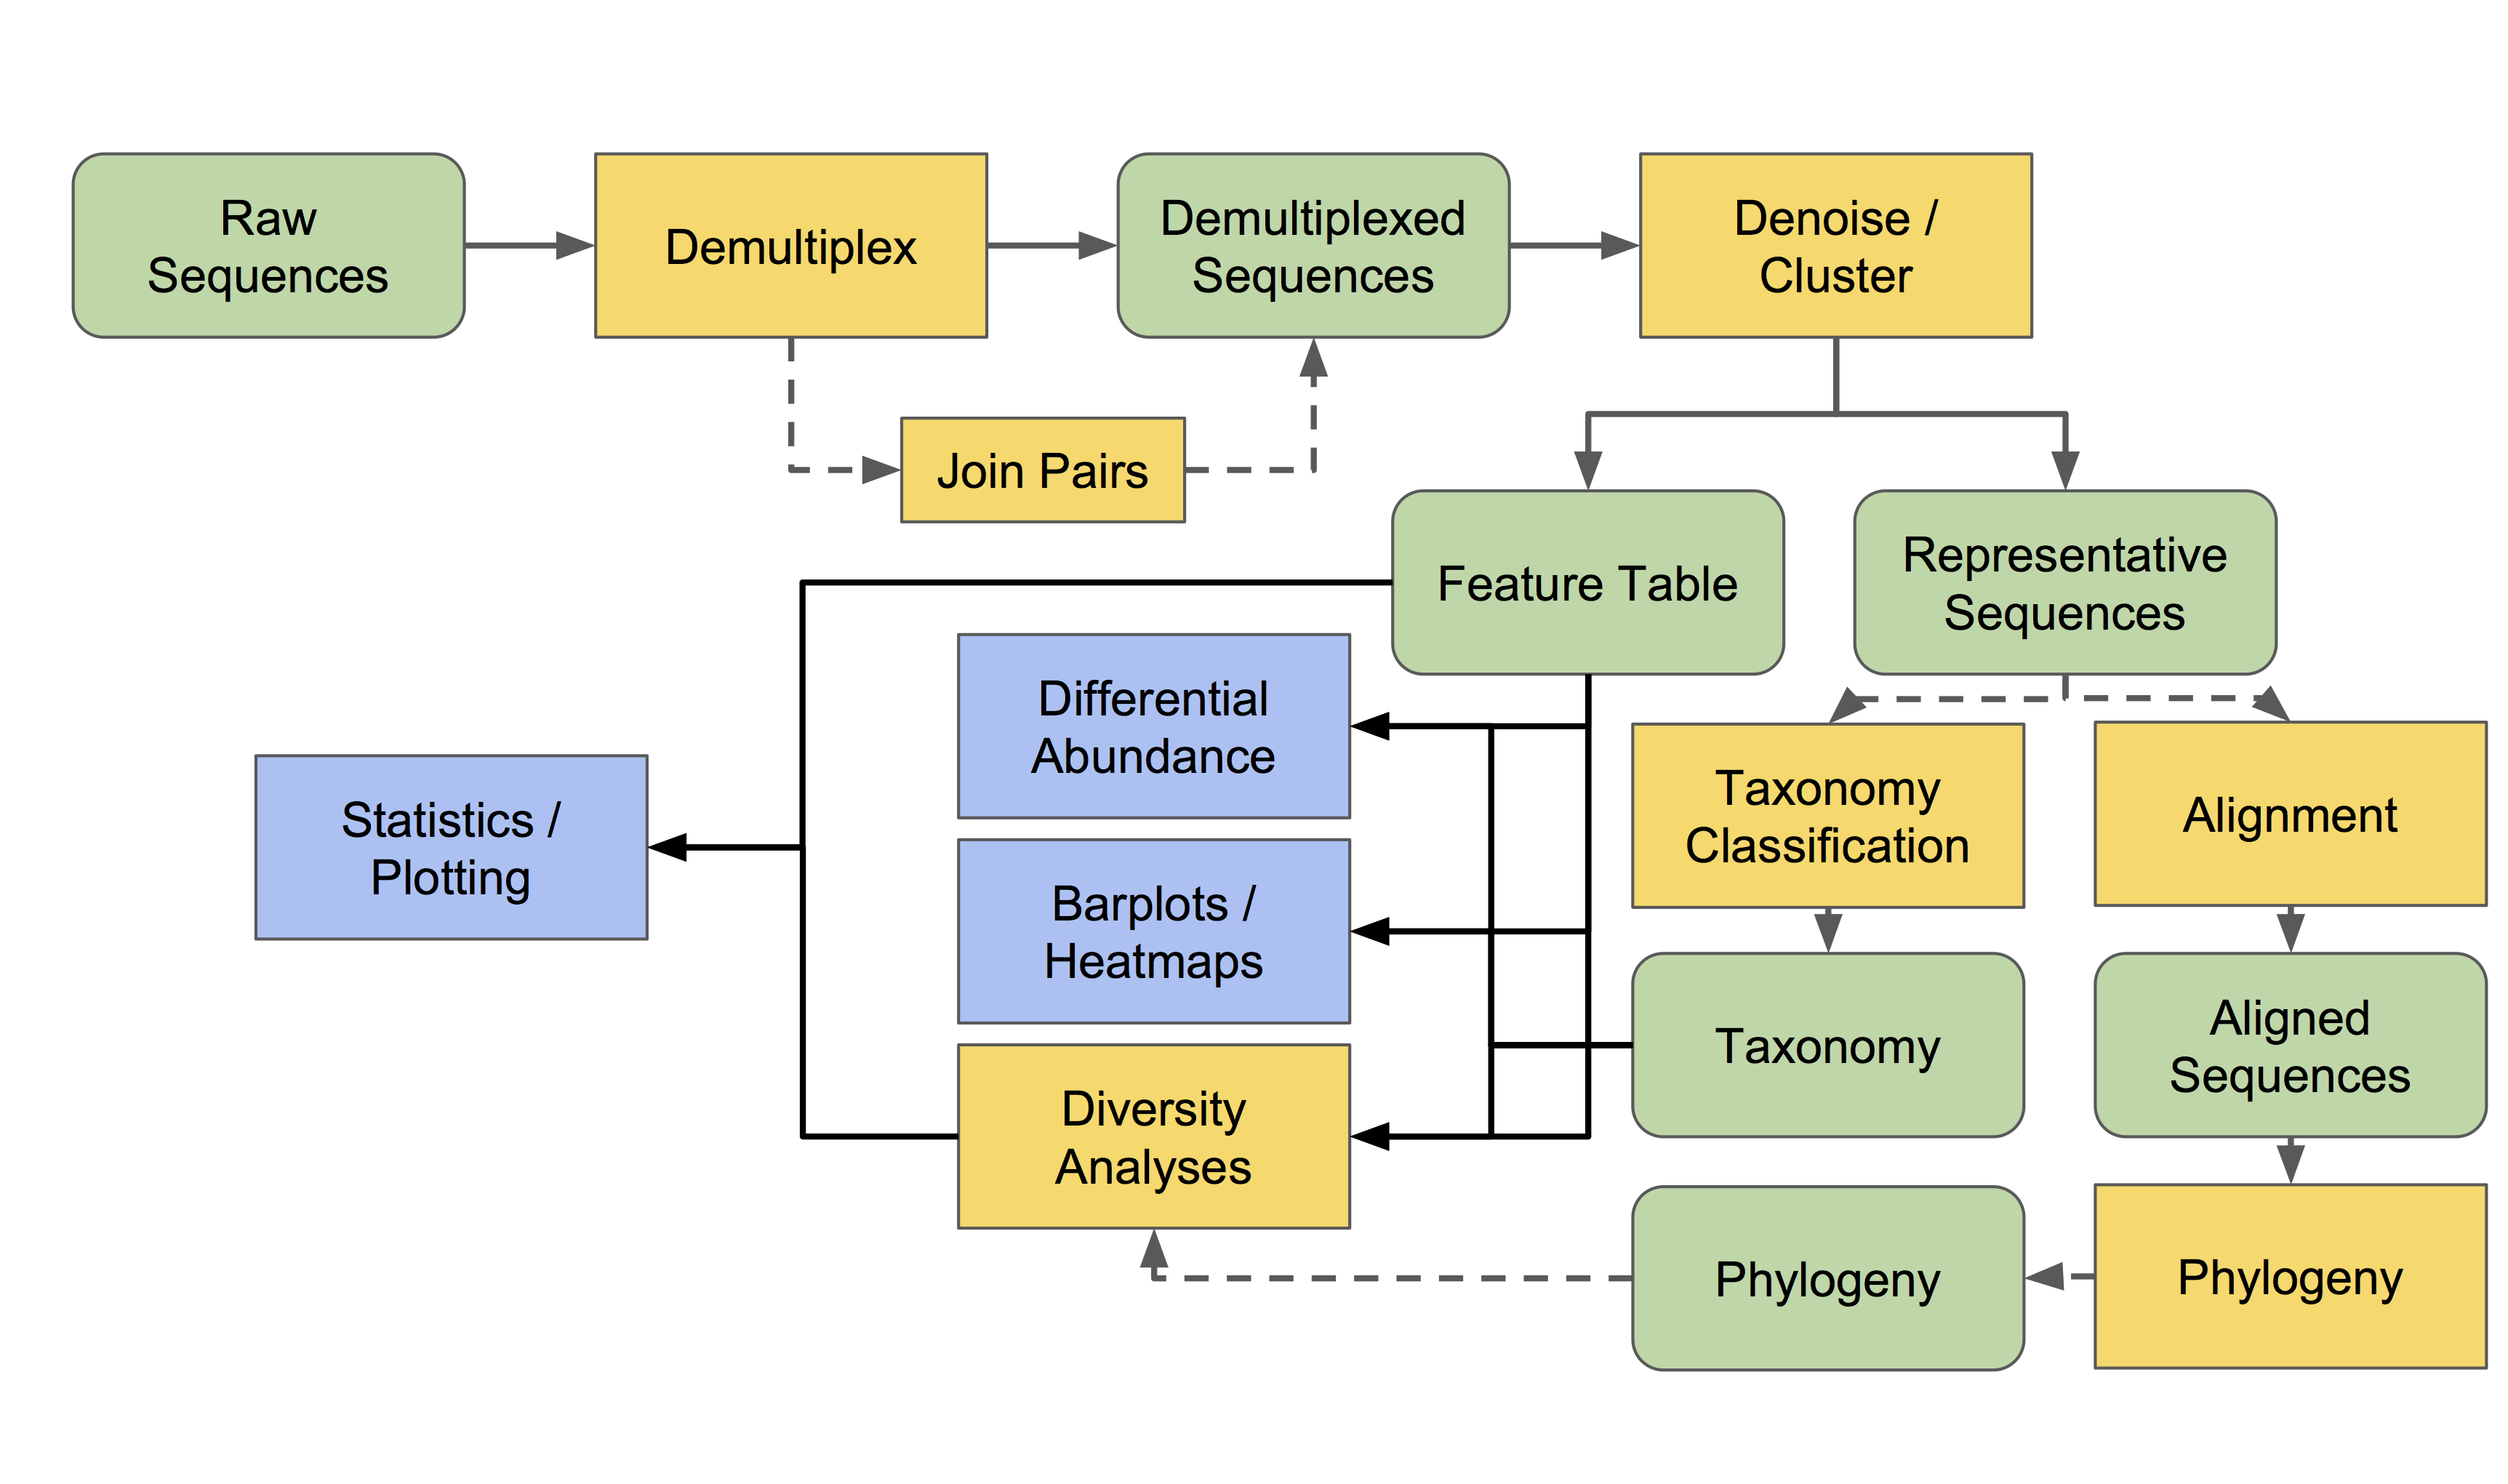
\includegraphics[width=0.8 \linewidth]{figures/qiime.png}
                \caption{A Theoretic Overview of QIIME2 Workflow \protect\cite{qiime1, qiime2}}
                \label{fig:qiime-workflow}
            \end{figure}

            \subsubsection{Denoising techniques}
                There are two denoising techniques provided by QIIME2: DADA2 \cite{DADA1} and Deblur \cite{deblur1}. The most meaningful difference between DADA2 and Deblur is the strategy that divides them into different variants (Figure \ref{fig:denosing-workflow}). DADA2 uses amplicon sequence variants (ASVs) that strictly divide sequences even one-base mismatch. However, Deblur uses operational taxonomic units (OTUs), considers the same taxonomies when they are 97 \% or more matched. We chose DADA2 rather than Deblur by the result of two reasons. First, DADA2 has internal filtering methods that cut the sequences with low-quality out. Second, DADA2 can be designated trimmed length both in forward and reverse.

                \begin{figure}[p]
                    \centering
                    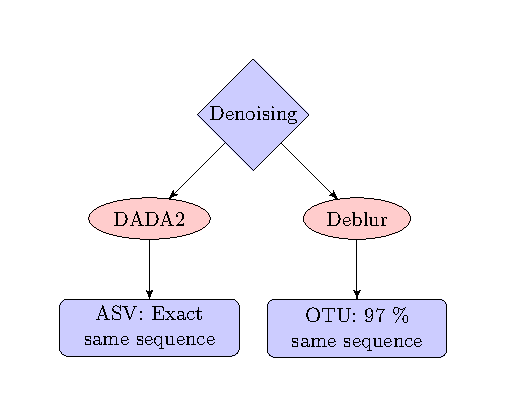
\includegraphics[width=0.5 \linewidth]{figures/denoising/denoising.pdf}
                    \caption{Denoising Techniques which provided by QIIME2}
                    \label{fig:denosing-workflow}
                \end{figure}

            \subsubsection{Taxonomy Classification}
                There are three taxonomy classification databases: Greengenes (GG) \cite{greengenes1}, SILVA \cite{silva1} and Human Oral Microbiome Database (HOMD) \cite{homd1}. The essential difference is its resolution. Previous researches have found that a higher accuracy at taxonomic levels above the genus level. However, accuracy drops at the species level \cite{performance1}.

                \begin{figure}[p]
                    \centering
                    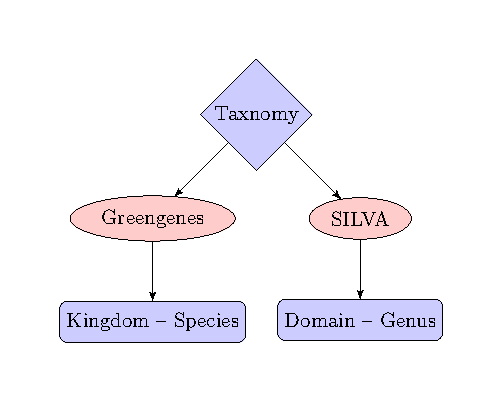
\includegraphics[width=0.5 \linewidth]{figures/taxonomy/taxonomy.pdf}
                    \caption{Taxonomy Classification which provided by QIIME2}
                    \label{fig:taxonomy-workflow}
                \end{figure}

            \subsubsection{Merging Denoising and Taxonomy Classification}
                After denoising and taxonomy classification steps, different IDs, such as ASVs or OTUs, have been identified as the single taxonomy. We considered those IDs as a single taxonomy (Figure \ref{fig:merging}).

                \begin{figure}[p]
                    \centering
                    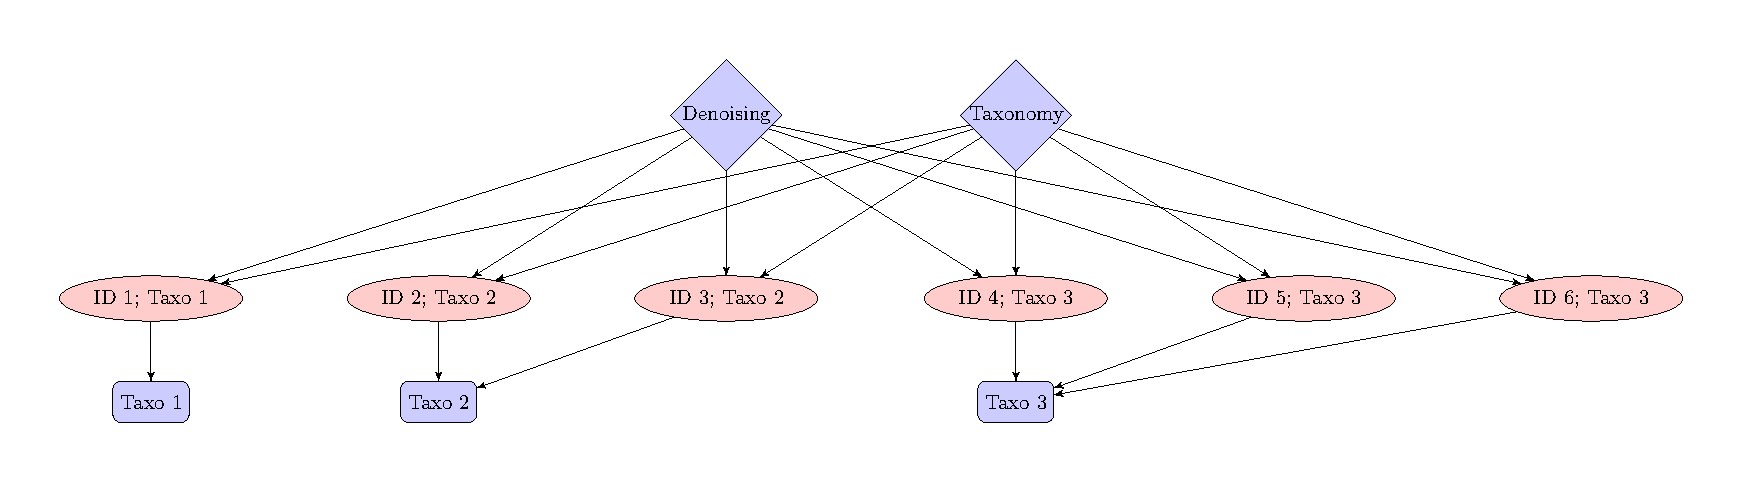
\includegraphics[width=0.8 \linewidth]{figures/Merging/merging.pdf}
                    \caption{Example Diagram for Merging Denoising and Taxonomy Classification}
                    \label{fig:merging}
                \end{figure}

            \subsubsection{Rarefaction}
                Rarefaction is a statistical method of estimating the number of species expected in a random sample taken from a collection \cite{rarefaction1}. Moreover, rarefaction allows comparisons of the species richness among communities. Thus, rarefaction is one of the best choices for normalization \cite{rarefaction2}.

            \subsubsection{Alpha-diversity}
                Alpha-diversity is a metric that shows the richness of taxa in a single community. QIIME2 provides four alpha-diversity indices:
                \begin{itemize}
                    \item Evenness index \cite{evenness1}.
                    \item Faith's phylogenetic diversity (Faith PD) \cite{faith1}.
                    \item Observed features.
                    \item Shannon's diversity index \cite{shannon1}.
                \end{itemize}

                The evenness index shows a measurement of diversity in a different type of community \cite{evenness1}. Faith's phylogenetic diversity index, however, indicates a qualitative evaluation of community richness. The index prefers species conservation that incorporates taxic diversity \cite{faith1}. Observed features index, as its name, is the number of detected features in the microbiome. Furthermore, Shannon's diversity index means a significant aspect of community richness \cite{shannon1}.

            \subsubsection{Beta-diversity}
                Beta-diversity is a metric that indicates the taxonomic differentiation among multiple communities. QIIME2 provides four beta-diversity indices:
                \begin{itemize}
                    \item Bray-Curtis distance index \cite{bray1}.
                    \item Jaccard distance index \cite{jaccard1}.
                    \item Unweighted UniFrac distance index \cite{unifrac1}.
                    \item Weighted UniFrac distance index \cite{unifrac1}.
                \end{itemize}

                Bray-Curtis distance index shows a quantitative measurement of community dissimilarity \cite{bray1}. Jaccard distance index, however, indicates an evaluation of local distribution among communities \cite{jaccard1}. UniFrac distance indices reveal measures of phylogenetic distances \cite{unifrac1}. The unweighted UniFrac distance index and the weighted UniFrac distance index promote qualitative and quantitative, respectively.

            \subsubsection{ANCOM}
                ANCOM (analysis for the composition of microbiomes) analyzes the architecture of the microbiome in multiple populations \cite{ANCOM1}. An example ANCOM volcano plot is figure \ref{fig:ancom-example}. In figure \ref{fig:ancom-example}, two metrics are clearly shown: clr and W. clr stands for centered $\log$ ratio, and W is a count of the number of sub-hypothesis which have passed for given species.

                \begin{figure}[p]
                    \centering
                    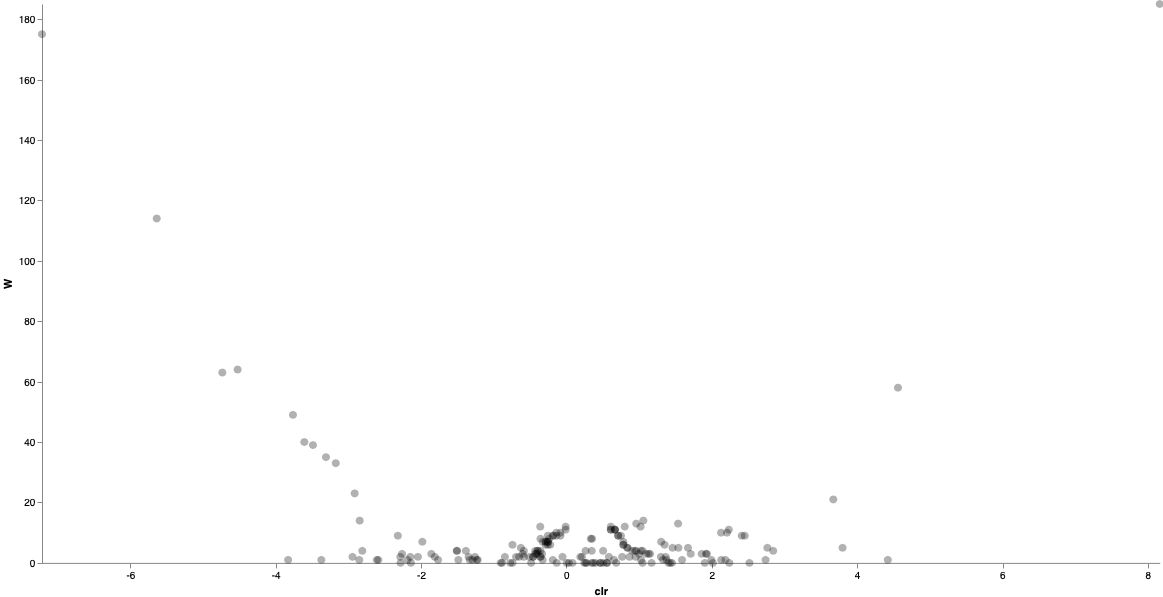
\includegraphics[width=0.8 \linewidth]{figures/ANCOM/example.png}
                    \caption{Example ANCOM Volcano Plot which Provided by QIIME2 \protect\cite{qiime1, qiime2}}
                    \label{fig:ancom-example}
                \end{figure}

        \subsection{Python Packages}
            \subsubsection{Pandas}
                Pandas is a Python package of rich data structures and tools for analyzing with structured data sets \cite{pandas1}.

            \subsubsection{Scikit-learn}
                Scikit-learn grants state-of-the-art implementation of many machine learning algorithms, while controlling an easy-to-use interface tightly integrated the Python code \cite{sklearn1}.

            \subsubsection{Matplotlib}
                Matplotlib is a Python graphics package which used for application development, interactive scripting and publication quality image generation \cite{matplotlib2}. Matplotlib, also, is designed to create simple plots with a few commands \cite{matplotlib1}.

            \subsubsection{Seaborn}
                Seaborn is a Python data visualization package which based on matplotlib, allows a high-level interface for displaying engaging and descriptive statistical graphics \cite{seaborn1}.

            \subsubsection{statannot}
                Statannot is a python package which computes statistical test and adds statistical annotations on violin plot generated by seaborn package.

        \subsection{t-SNE}
            t-SNE (t-distributed stochastic neighbor embedding) reveals high-dimensional data in a location in a two-dimensional map \cite{tSNE1}. Figure \ref{fig:tsne-example} is example of t-SNE with hand-writing digits \cite{tSNE1}. In figure \ref{fig:tsne-example}, all 10 digits are grouped into 10 groups clearly; some hand-writings, however, are classified into wrong groups due to their similar shapes, such as 0 and 6.

            \begin{figure}[p]
                \centering
                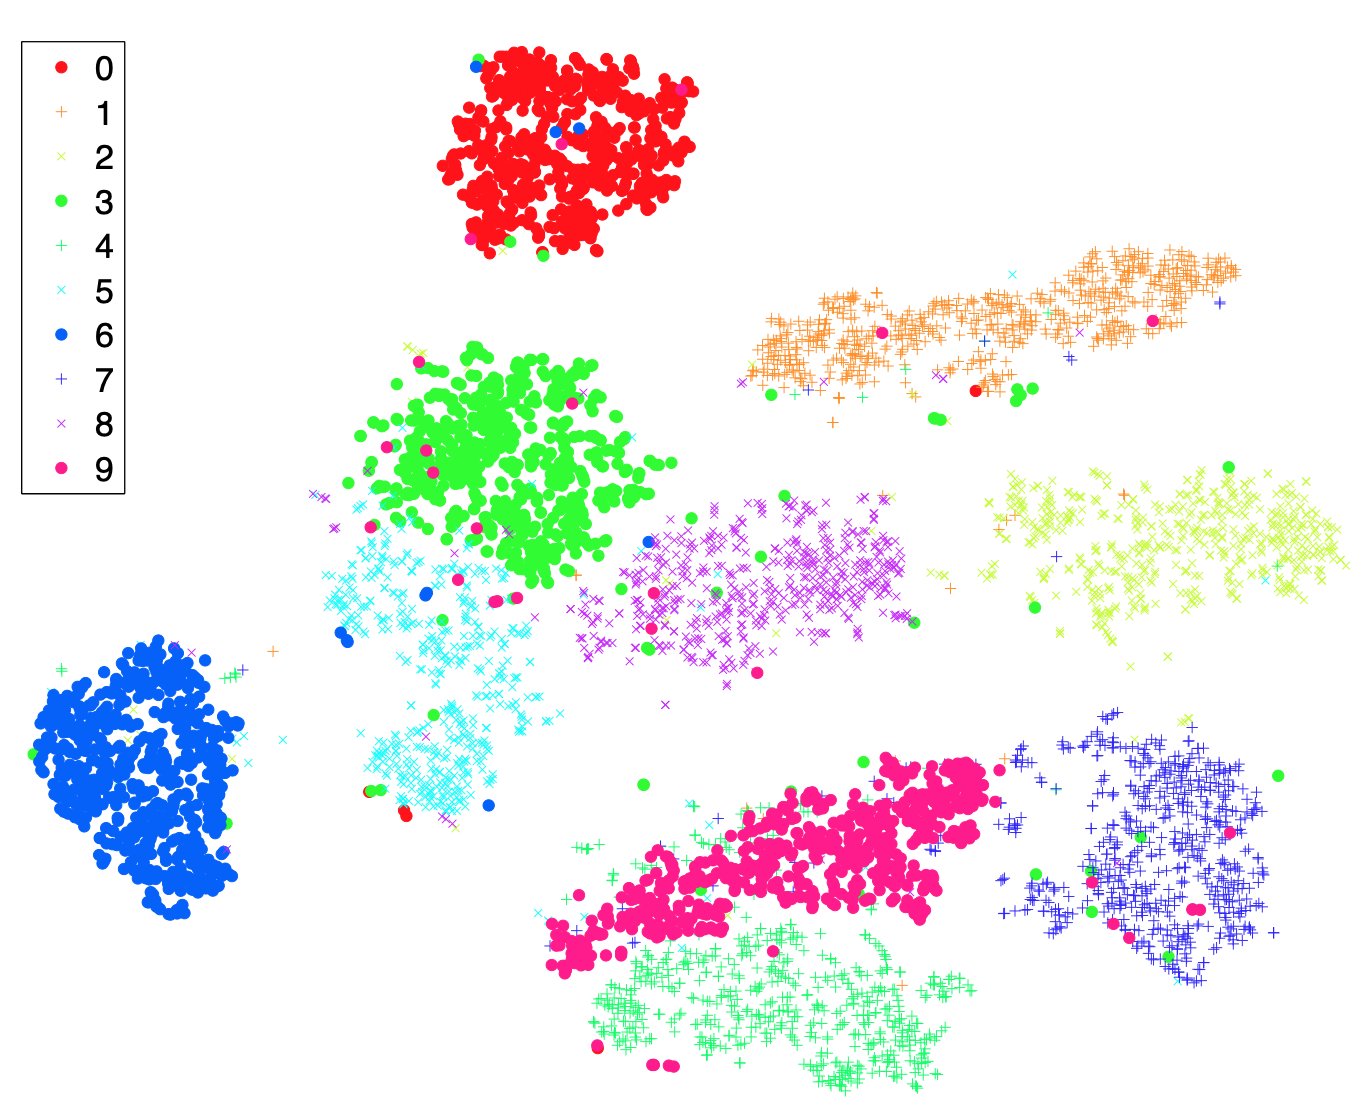
\includegraphics[width=0.4 \linewidth]{figures/tSNE.png}
                \caption{Visualization by t-SNE \protect\cite{tSNE1}}
                \label{fig:tsne-example}
            \end{figure}

        \subsection{Classification}
            In machine learning, classification is one of the supervised problems. Classifier identifies a class of new observations, depends on training observations.

            In this study, classification will be carried out as figure \ref{fig:classification}; and the third step in figure \ref{fig:classification} is demonstrated in minute detail as figure \ref{fig:deciding-best}. Note that the first step in figure \ref{fig:classification} is optional: due to tables herein-after, such as table\ref{tb:alpha-evenness-dada2}, show that no statistically significant differences between healthy samples and early periodontitis samples and between moderate periodontitis samples and severe periodontitis samples.

            Moreover, evaluations of classification algorithm are carried out with derivations from confusion matrix (table \ref{tb:confusion-matrix}):

            \begin{itemize}
                \item Accuracy (ACC) $ = \frac{TP + TN}{TP + TN + FP + FN}$
                \item Balanced Accuracy (BA) $ = \frac{TP}{2 \times (TP + FN)} + \frac{TN}{2 \times (TN + FP)}$
                \item Sensitivity (SEN) $ = \frac{TP}{TP + FN}$
                \item Specificity (SPE) $ = \frac{TN}{TN + FP}$
                \item Precision (PRE) $ = \frac{TP}{TP + FP}$
            \end{itemize}

            \begin{table}[p]
                \centering
                \caption{Confusion Matrix}
                \label{tb:confusion-matrix}
                \begin{tabular}{c|c|cc}
                    \multicolumn{2}{c|}{\multirow{2}{*}{}} & \multicolumn{2}{c}{Actual Class} \\ \cline{3-4}
                    \multicolumn{2}{c|}{} & Positive & Negative \\ \hline
                    \multirow{2}{*}{Predicted Class} & Positive & True Positive (TP) & False Positive (FP) \\
                    & Negative & False Negative (FN) & True Negative (TN)
                \end{tabular}
            \end{table}

            \begin{figure}[p]
                \centering
                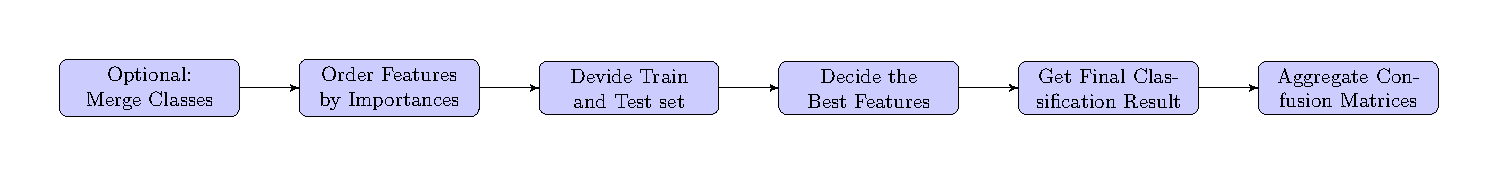
\includegraphics[width=0.8 \linewidth]{figures/Classifier/classifier.pdf}
                \caption{Workflow of Classification}
                \label{fig:classification}
            \end{figure}

            \begin{figure}[p]
                \centering
                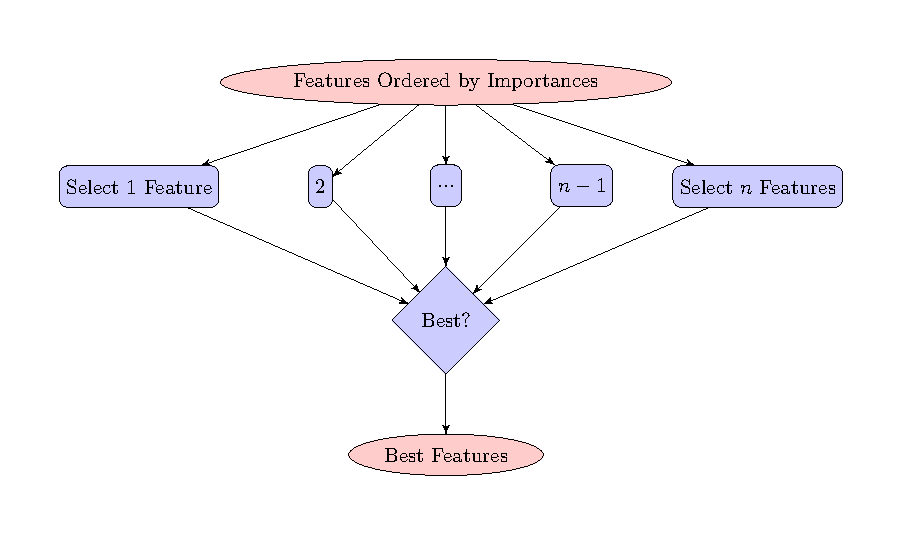
\includegraphics[width=0.6 \linewidth]{figures/Classifier/best.pdf}
                \caption{Deciding the Best Features}
                \label{fig:deciding-best}
            \end{figure}

            \subsubsection{Random Forest Classification}
                As figure \ref{fig:classification}, importance of features have to be derived by classifier. Random Forest classifier \cite{RandomForest1} can get this information, and is used frequently by researchers. Hence, Random Forest classifier will be carried out with every class (Figure \ref{fig:RF-whole-workflow}) or with merged classes (Figure \ref{fig:RF-merging-workflow}).

                \begin{figure}[p]
                    \centering
                    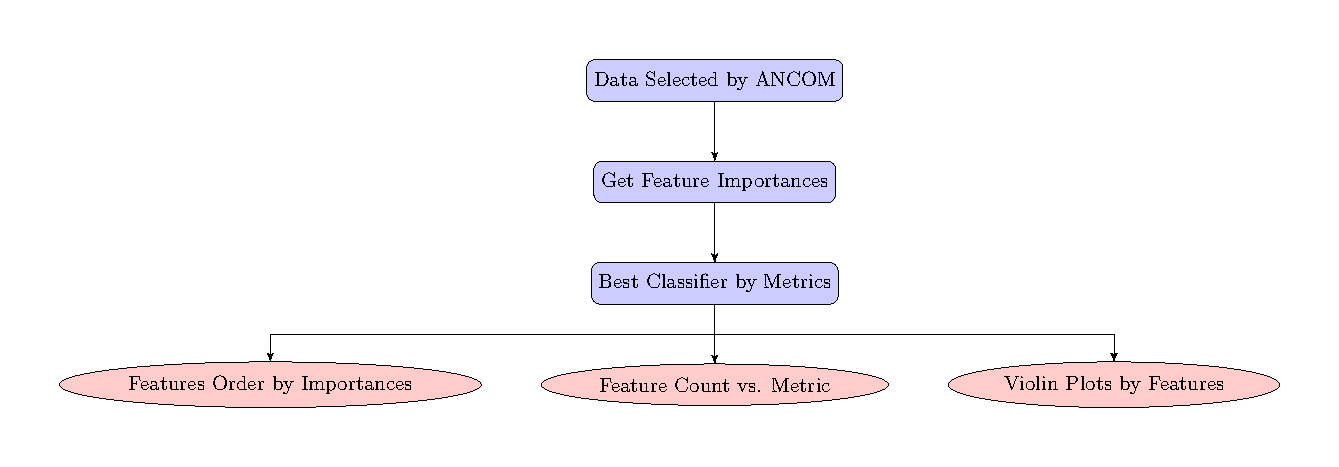
\includegraphics[width=0.6 \linewidth]{figures/RandomForest/whole.pdf}
                    \caption{Random Forest Classifier Workflow}
                    \label{fig:RF-whole-workflow}
                \end{figure}

                \begin{figure}[p]
                    \centering
                    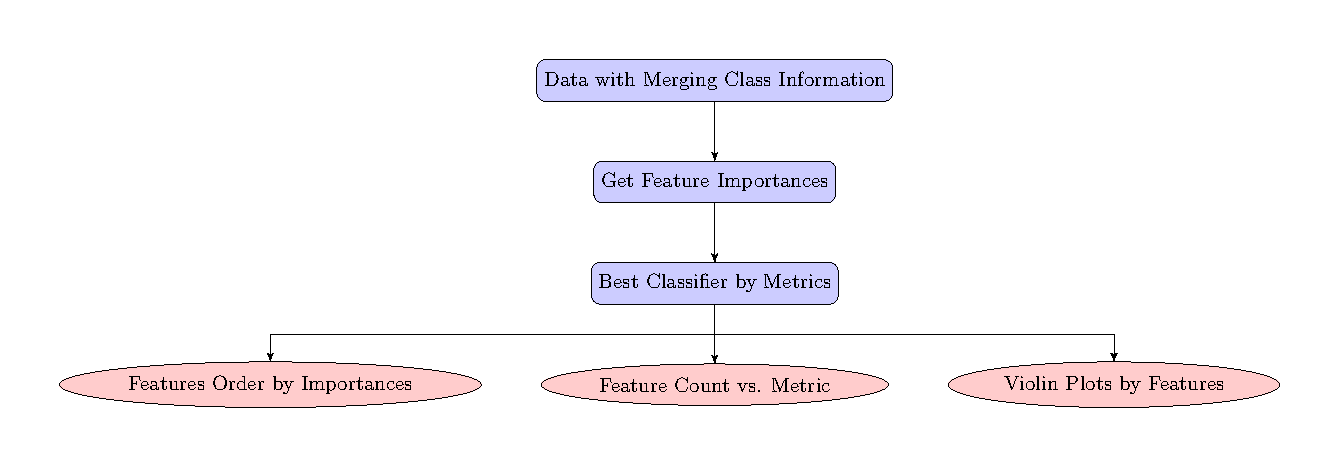
\includegraphics[width=0.6 \linewidth]{figures/RandomForest/merge.pdf}
                    \caption{Random Forest Classifier Workflow with Merging}
                    \label{fig:RF-merging-workflow}
                \end{figure}

    \section{Results}
        \subsection{Quality Filter}
            Longer sequences have more fallen sequence quality than shorter. Thus, sequences which longer than threshold should be trimmed out due to their low quality. However, gold-standard strategy for deciding the threshold does not exist; the threshold is set as longest sequence length which have half of sequences have greater than 30 quality score. Hence, sequence quality plot is shown as figure \ref{fig:sequence-quality}; trimmed length in forward reads is 300, and trimmed length in reverse reads is 265.

            \begin{figure}[p]
                \centering
                $\begin{array}{cc}
                    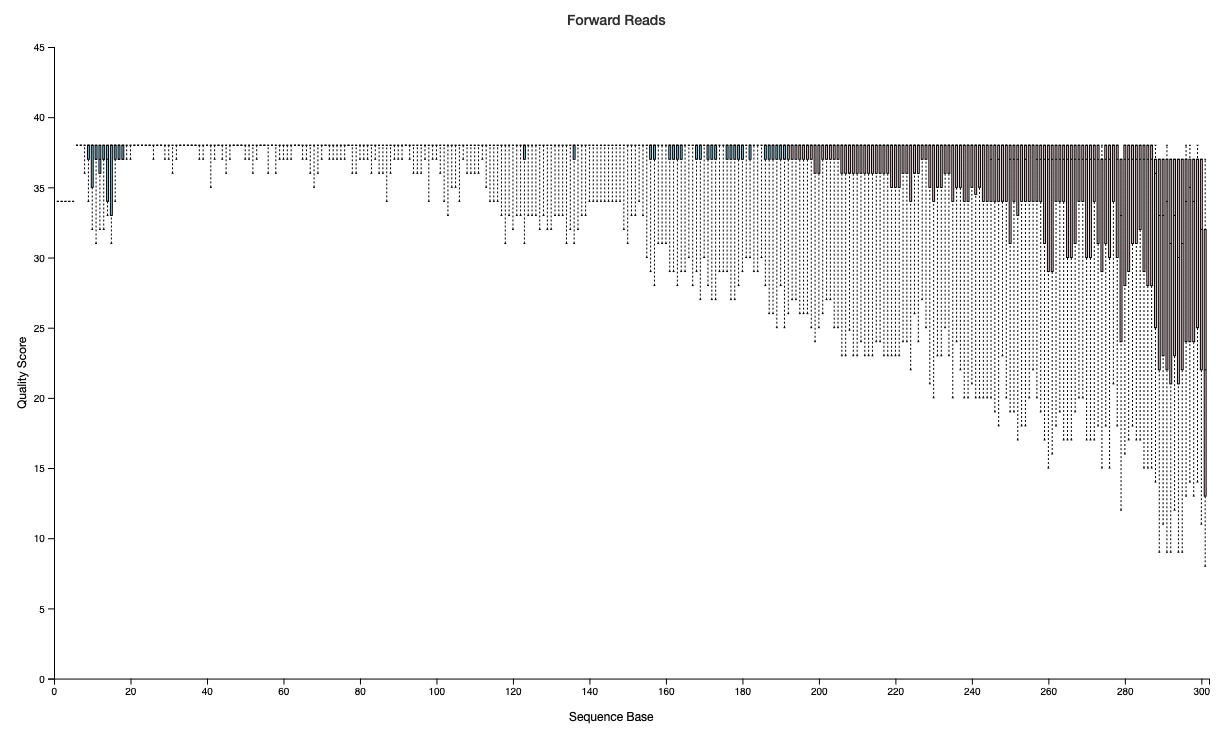
\includegraphics[width=0.4 \linewidth]{figures/QualityFilter/Forward.png}
                    &
                    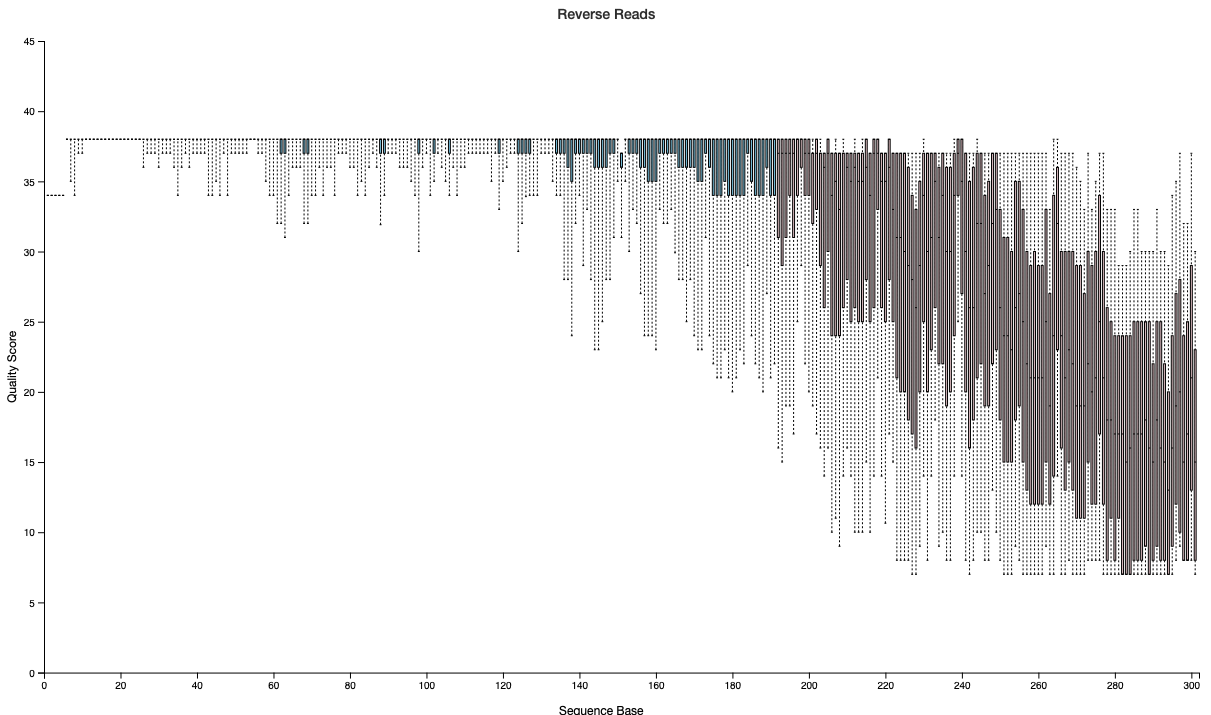
\includegraphics[width=0.4 \linewidth]{figures/QualityFilter/Reverse.png}
                    \\
                    \mbox{(a) Forward Reads} & \mbox{(b) Reverse Reads} \\
                \end{array}$
                \caption{Sequence Quality Plot}
                \label{fig:sequence-quality}
            \end{figure}

        \subsection{Rarefaction}
            Sampling depth should be decided for rarefaction. Gold-standard method for determining sampling depth is minimum frequency in the samples. Hence, sampling depth with DADA2 is 3,786 (Figure \ref{fig:frequency-sample-dada2}), and sampling depth with Deblur is 7,253 (Figure \ref{fig:frequency-sample-deblur}).

            \begin{figure}[p]
                \centering
                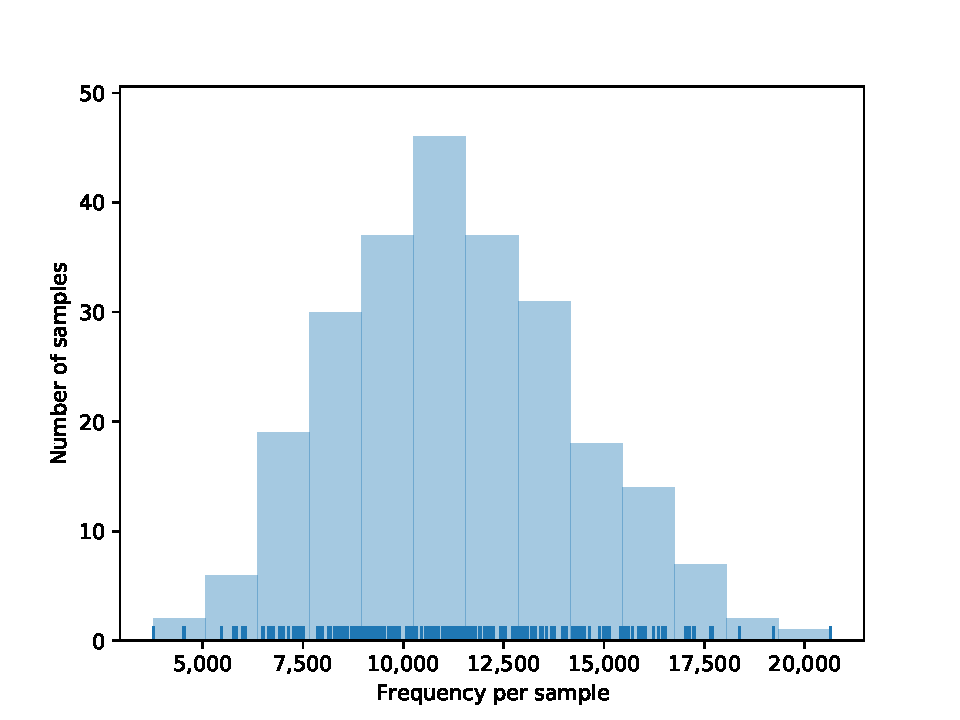
\includegraphics[width=0.6 \linewidth]{figures/Rarefaction/DADA.pdf}
                \caption{Frequency and Number per Sample by DADA2}
                \label{fig:frequency-sample-dada2}
            \end{figure}

            \begin{figure}[p]
                \centering
                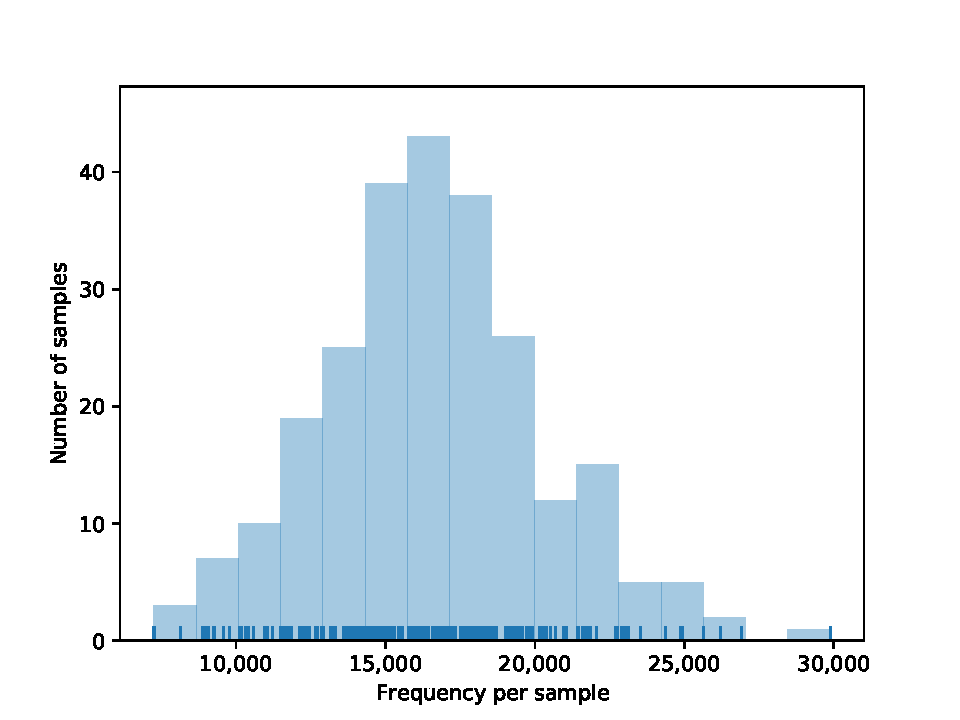
\includegraphics[width=0.6 \linewidth]{figures/Rarefaction/Deblur.pdf}
                \caption{Frequency and Number per Sample by Deblur}
                \label{fig:frequency-sample-deblur}
            \end{figure}

        \subsection{Alpha-diversity}

            \begin{table}[p]
                \centering
                \caption{Kruskal-Wallis Tests among All Group with DADA2}
                \label{tb:alpha-all-dada2}
                \csvautobooktabular{csv/AlphaDiversity/DADA2/all.csv}
            \end{table}

            \begin{table}[p]
                \centering
                \caption{Kruskal-Wallis Tests from Evenness Index with DADA2}
                \label{tb:alpha-evenness-dada2}
                \csvautobooktabular{csv/AlphaDiversity/DADA2/evenness.csv}
            \end{table}

            \begin{table}[p]
                \centering
                \caption{Kruskal-Wallis Tests from Faith PD Index with DADA2}
                \label{tb:alpha-faith-dada2}
                \csvautobooktabular{csv/AlphaDiversity/DADA2/faith.csv}
            \end{table}

            \begin{table}[p]
                \centering
                \caption{Kruskal-Wallis Tests from Observed Features Index with DADA2}
                \label{tb:alpha-observed-dada2}
                \csvautobooktabular{csv/AlphaDiversity/DADA2/observed.csv}
            \end{table}

            \begin{table}[p]
                \centering
                \caption{Kruskal-Wallis Tests from Shannon's Diversity Index with DADA2}
                \label{tb:alpha-shannon-dada2}
                \csvautobooktabular{csv/AlphaDiversity/DADA2/shannon.csv}
            \end{table}

            \begin{figure}[p]
                \centering
                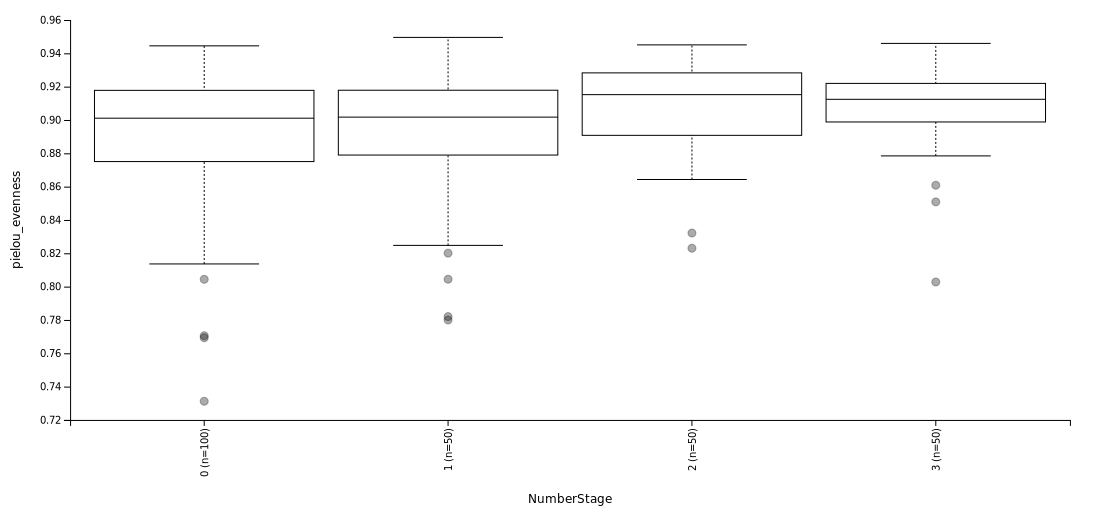
\includegraphics[width=0.8 \linewidth]{figures/AlphaDiversity/DADA2/evenness.png}
                \caption{Evenness Index from DADA2}
                \label{fig:evenness-dada2}
            \end{figure}

            \begin{figure}[p]
                \centering
                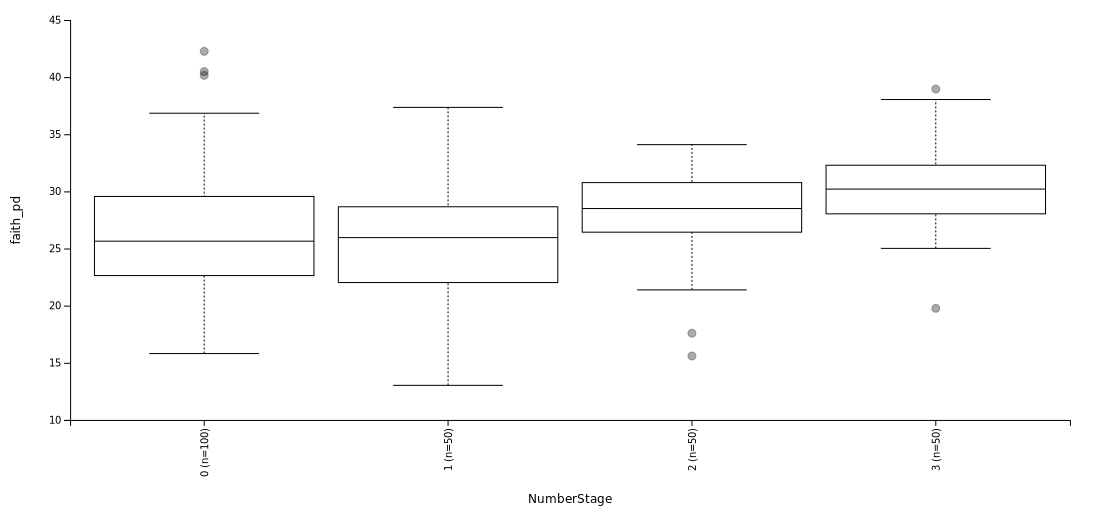
\includegraphics[width=0.8 \linewidth]{figures/AlphaDiversity/DADA2/faith.png}
                \caption{Faith PD Index from DADA2}
                \label{fig:faith-dada2}
            \end{figure}

            \begin{figure}[p]
                \centering
                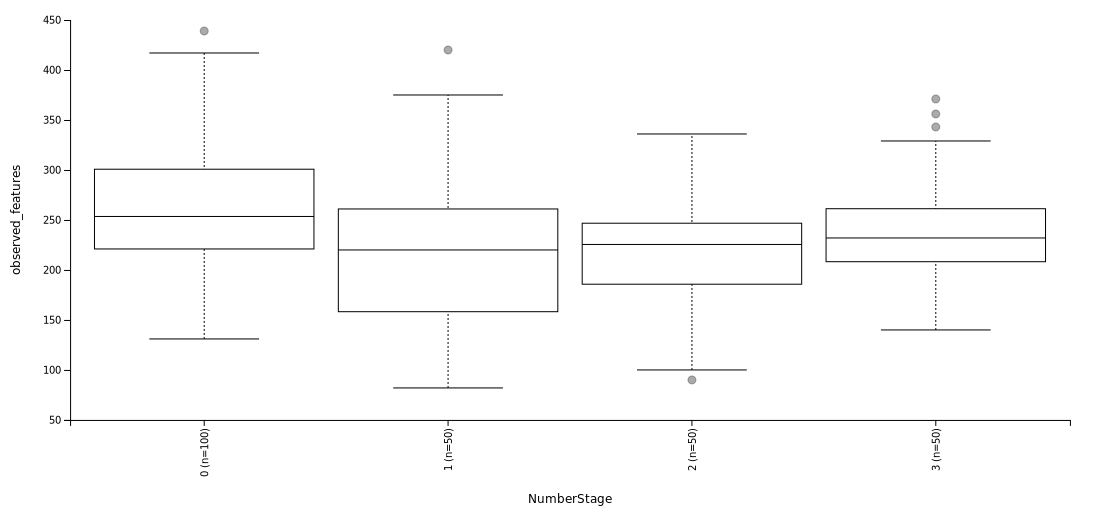
\includegraphics[width=0.8 \linewidth]{figures/AlphaDiversity/DADA2/observed.png}
                \caption{Observed Features Index from DADA2}
                \label{fig:observed-dada2}
            \end{figure}

            \begin{figure}[p]
                \centering
                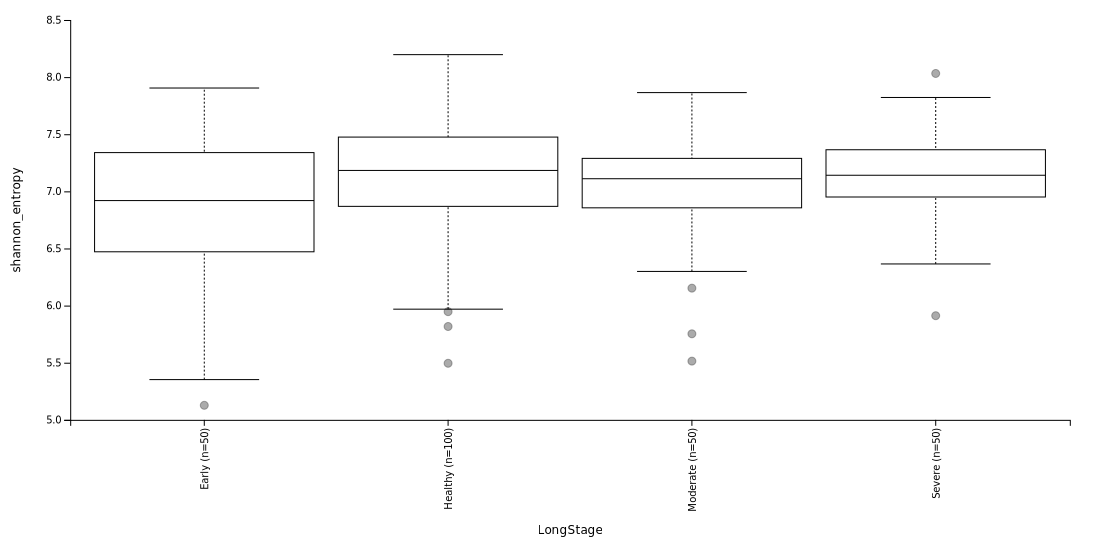
\includegraphics[width=0.8 \linewidth]{figures/AlphaDiversity/DADA2/shannon.png}
                \caption{Shannon's Diversity Index from DADA2}
                \label{fig:shannon-dada2}
            \end{figure}

        \subsection{Beta-diversity}

            \begin{table}[p]
                \centering
                \caption{Bray-Curtis Distance Index with DADA2}
                \label{tb:bray-dada2}
                \csvautobooktabular{csv/BetaDiversity/DADA2/Bray.csv}
            \end{table}

            \begin{table}[p]
                \centering
                \caption{Jaccard Distance Index with DADA2}
                \label{tb:jaccard-dada2}
                \csvautobooktabular{csv/BetaDiversity/DADA2/Jaccard.csv}
            \end{table}

            \begin{table}[p]
                \centering
                \caption{Unweighted UniFrac Distance Index with DADA2}
                \label{tb:unweighted-dada2}
                \csvautobooktabular{csv/BetaDiversity/DADA2/UnweightedUniFrac.csv}
            \end{table}

            \begin{table}[p]
                \centering
                \caption{Weighted UniFrac Distance Index with DADA2}
                \label{tb:weighted-dada2}
                \csvautobooktabular{csv/BetaDiversity/DADA2/WeightedUniFrac.csv}
            \end{table}

            \begin{figure}[p]
                \centering
                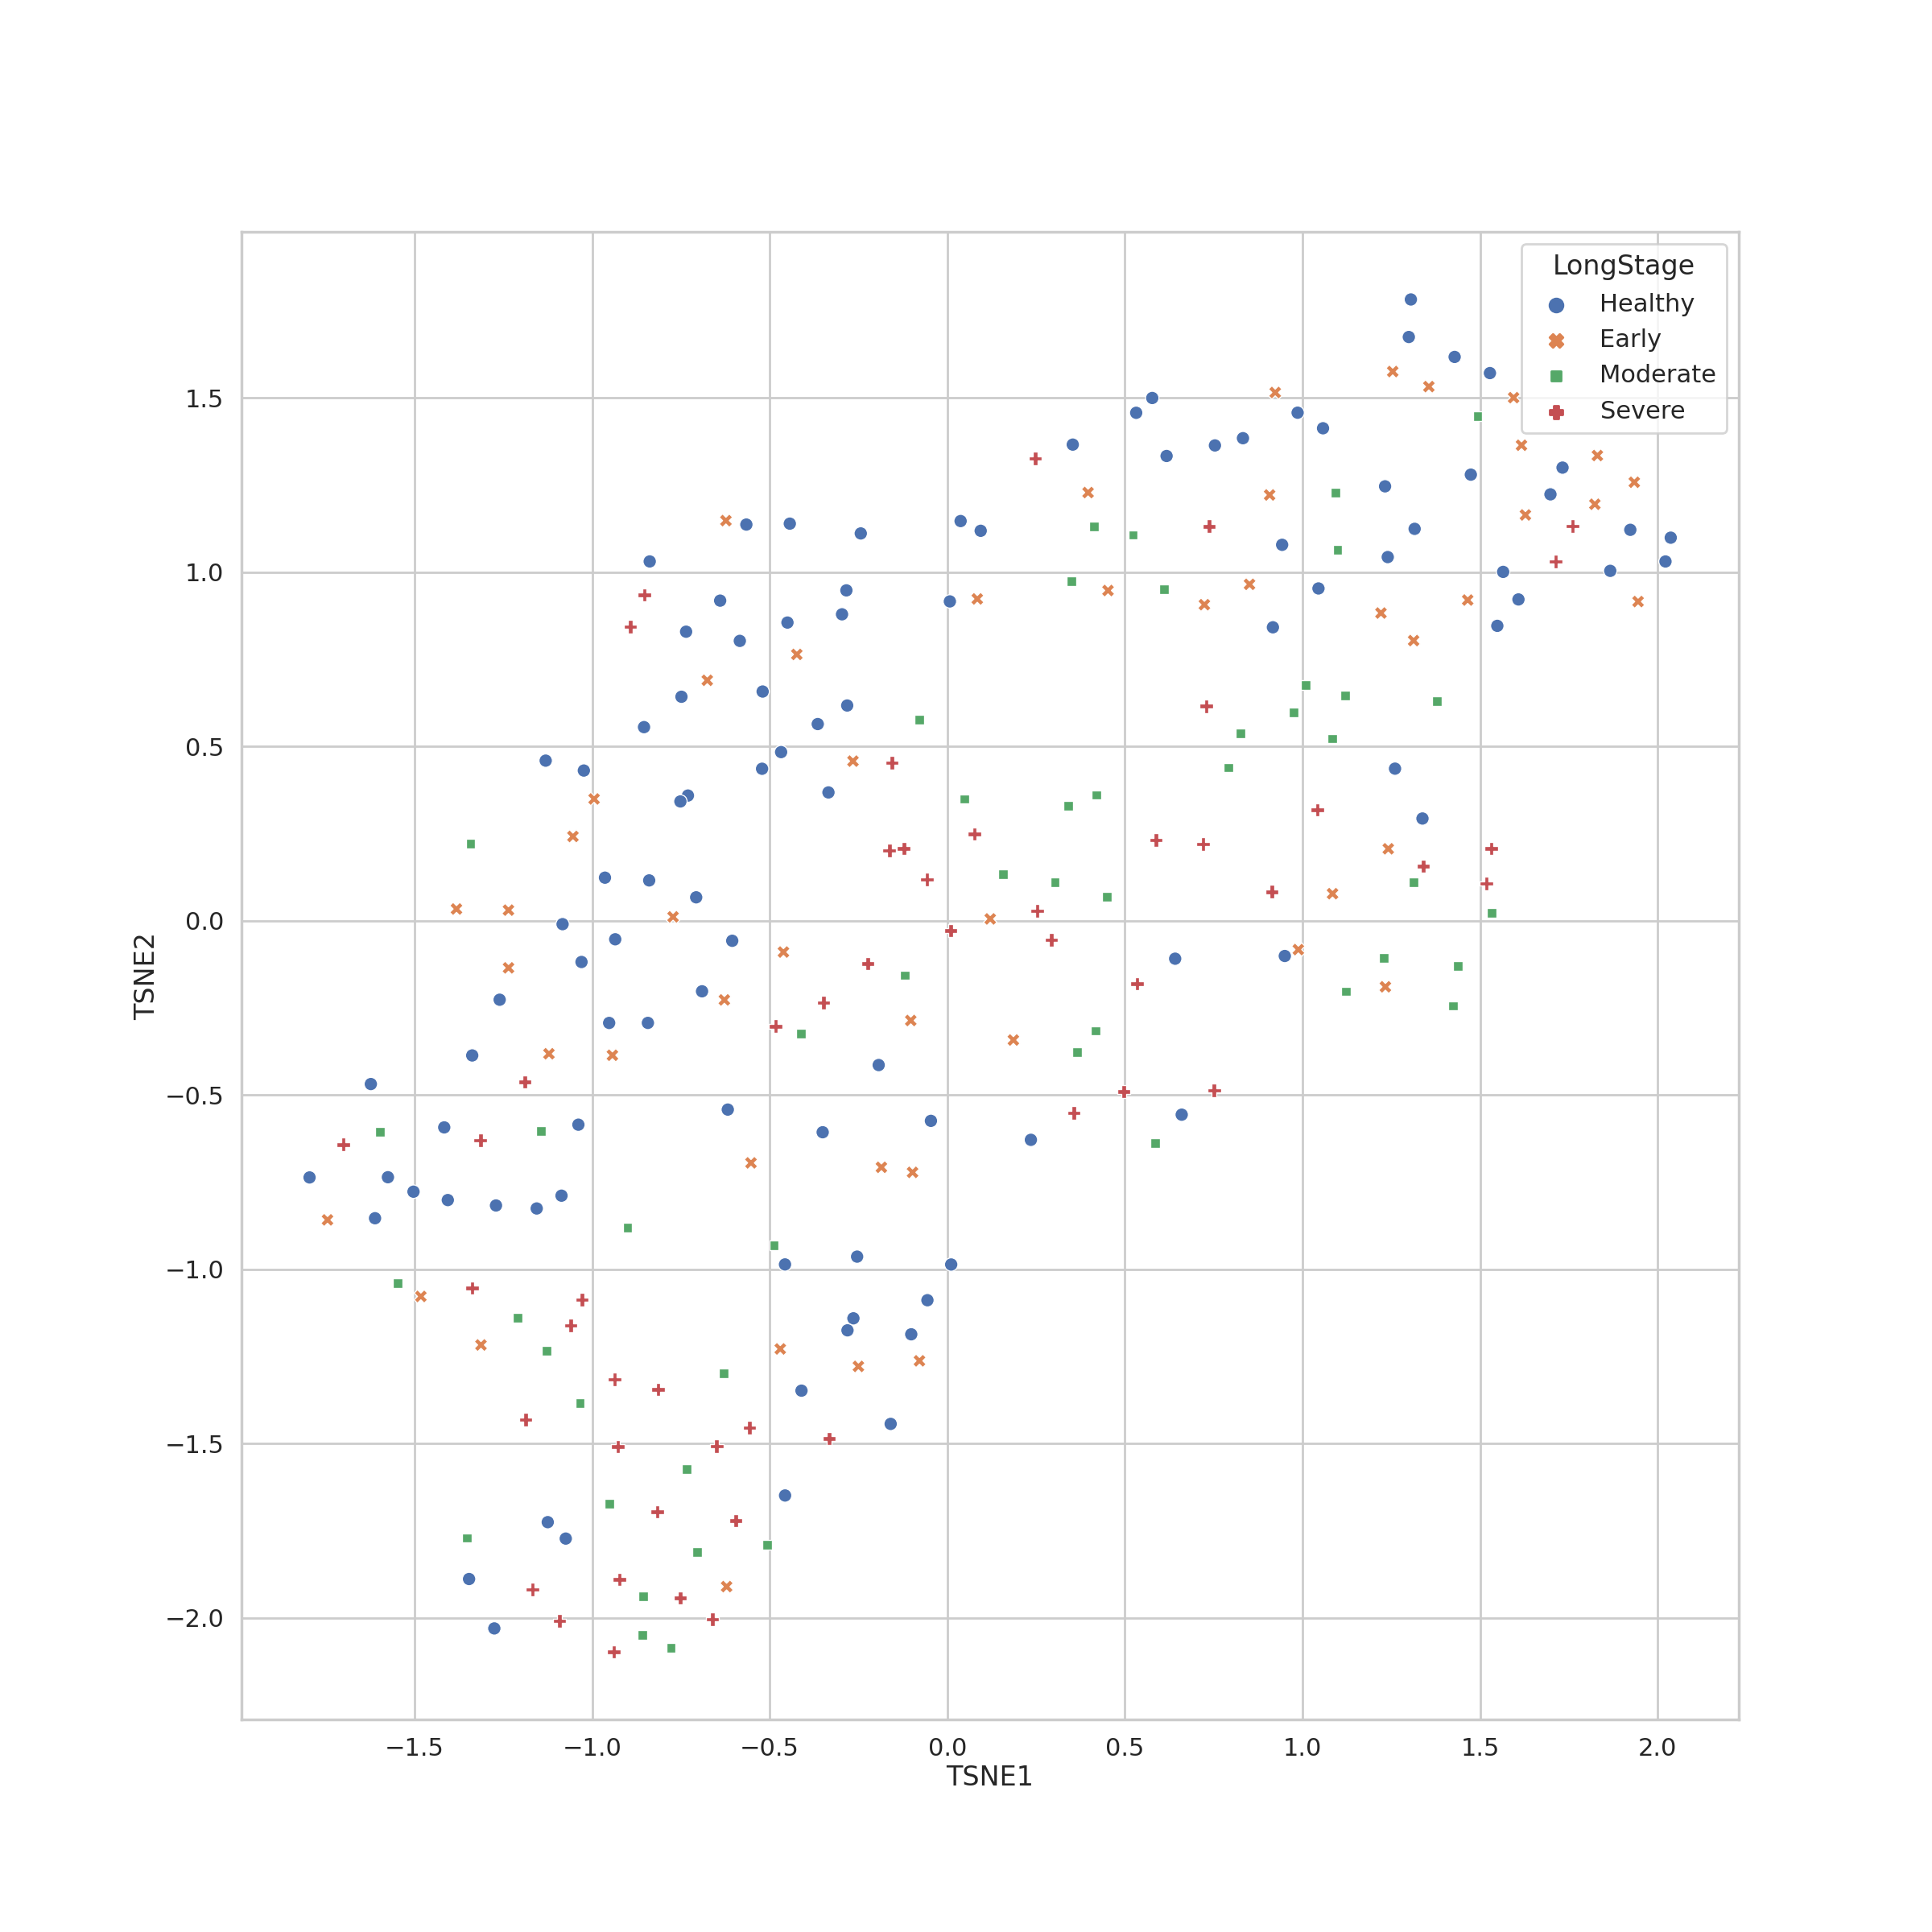
\includegraphics[width=0.6 \linewidth]{figures/BetaDiversity/DADA2.bray_curtis.png}
                \caption{t-SNE Plot from Bray-Curtis Distance Index with DADA2}
                \label{fig:tsne-bray-dada2}
            \end{figure}

            \begin{figure}[p]
                \centering
                $\begin{array}{cc}
                    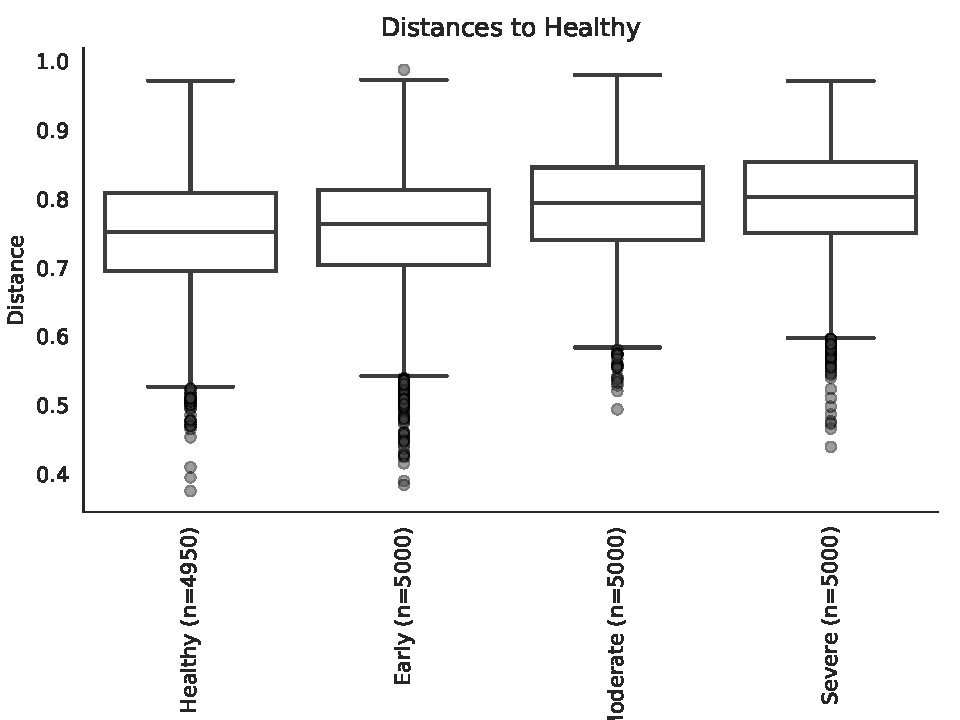
\includegraphics[width=0.4 \linewidth]{figures/BetaDiversity/DADA2/Bray/Healthy.pdf}
                    &
                    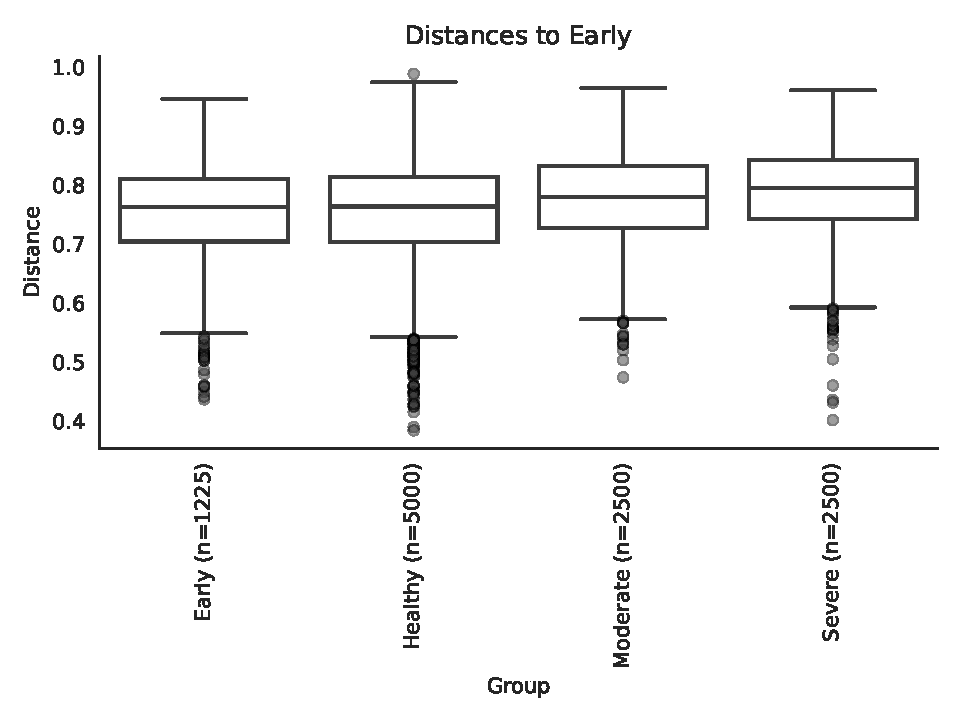
\includegraphics[width=0.4 \linewidth]{figures/BetaDiversity/DADA2/Bray/Early.pdf}
                    \\
                    \mbox{(a) Healthy} & \mbox{(b) Early} \\

                    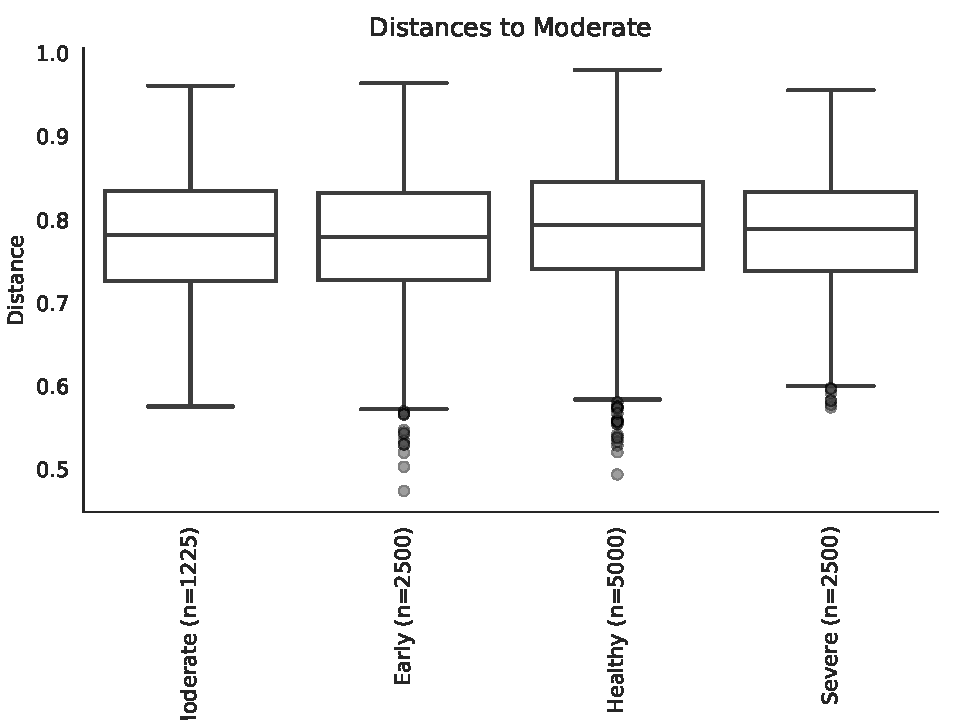
\includegraphics[width=0.4 \linewidth]{figures/BetaDiversity/DADA2/Bray/Moderate.pdf}
                    &
                    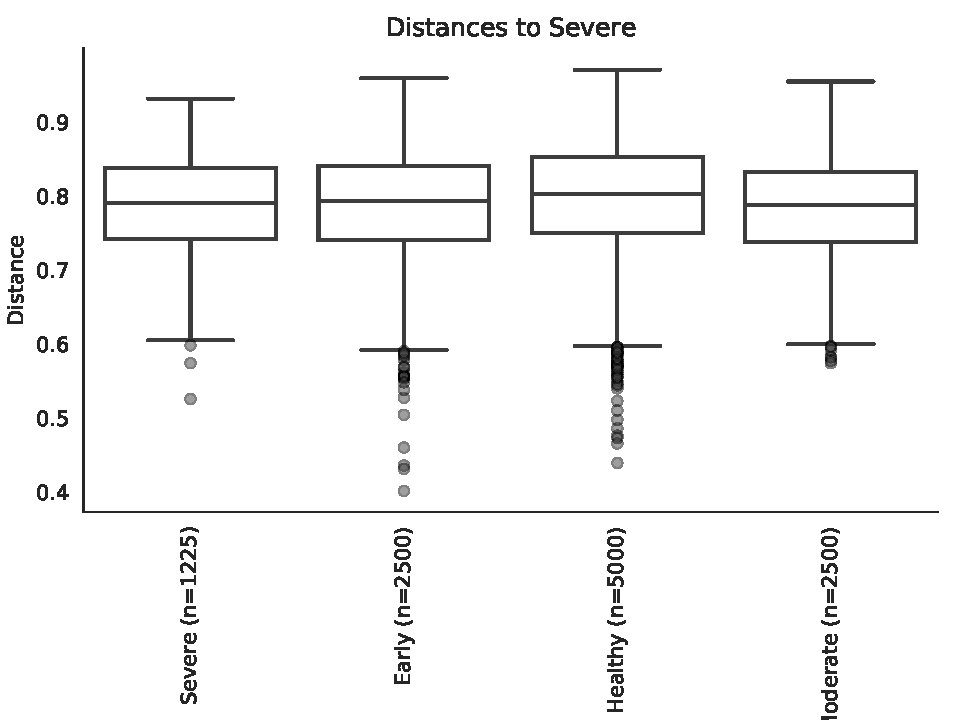
\includegraphics[width=0.4 \linewidth]{figures/BetaDiversity/DADA2/Bray/Severe.pdf}
                    \\
                    \mbox{(c) Moderate} & \mbox{(d) Severe} \\
                \end{array}$
                \caption{Bray-Curtis Distance Index with DADA2}
                \label{fig:bray-dada2}
            \end{figure}

            \begin{figure}[p]
                \centering
                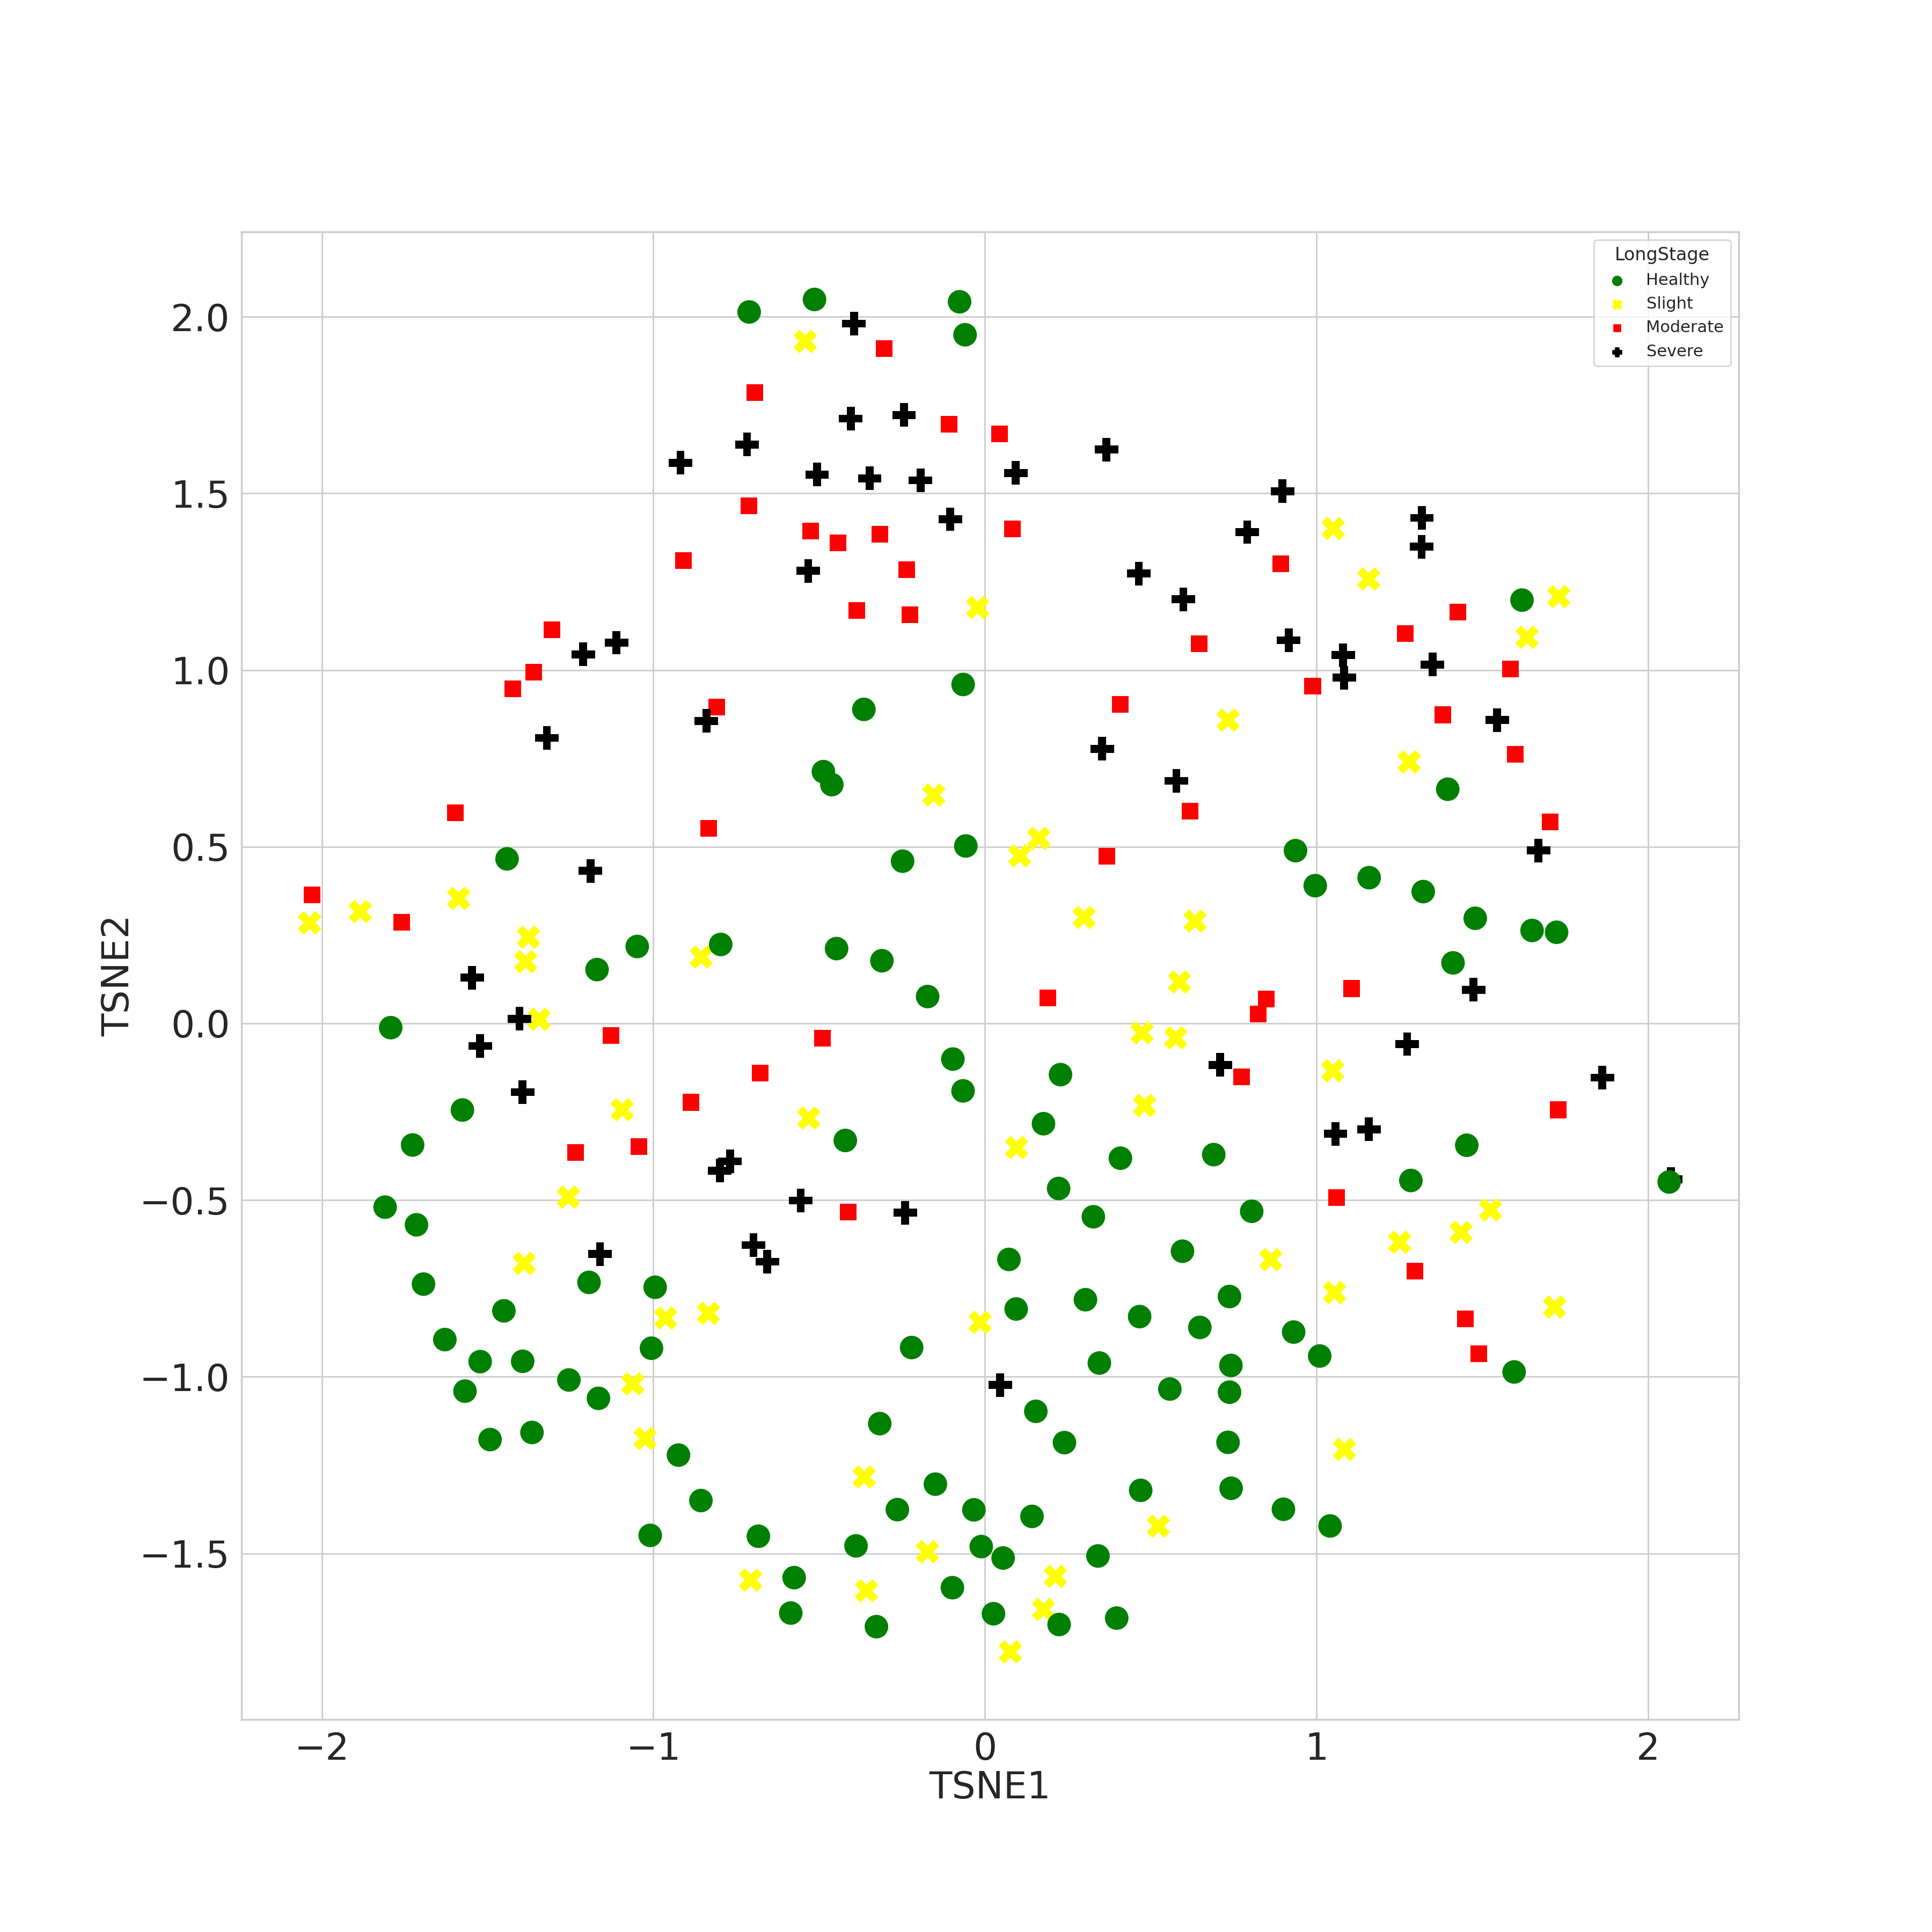
\includegraphics[width=0.6 \linewidth]{figures/BetaDiversity/DADA2.jaccard.png}
                \caption{t-SNE Plot from Jaccard Distance Index with DADA2}
                \label{fig:tsne-jaccard-dada2}
            \end{figure}

            \begin{figure}[p]
                \centering
                $\begin{array}{cc}
                    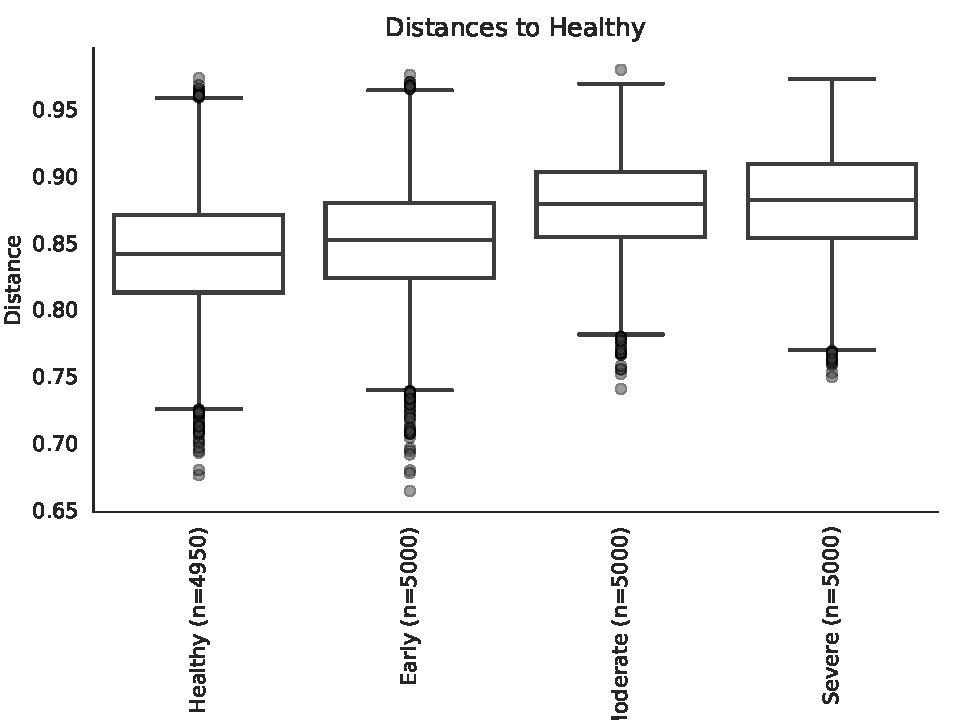
\includegraphics[width=0.4 \linewidth]{figures/BetaDiversity/DADA2/Jaccard/Healthy.pdf}
                    &
                    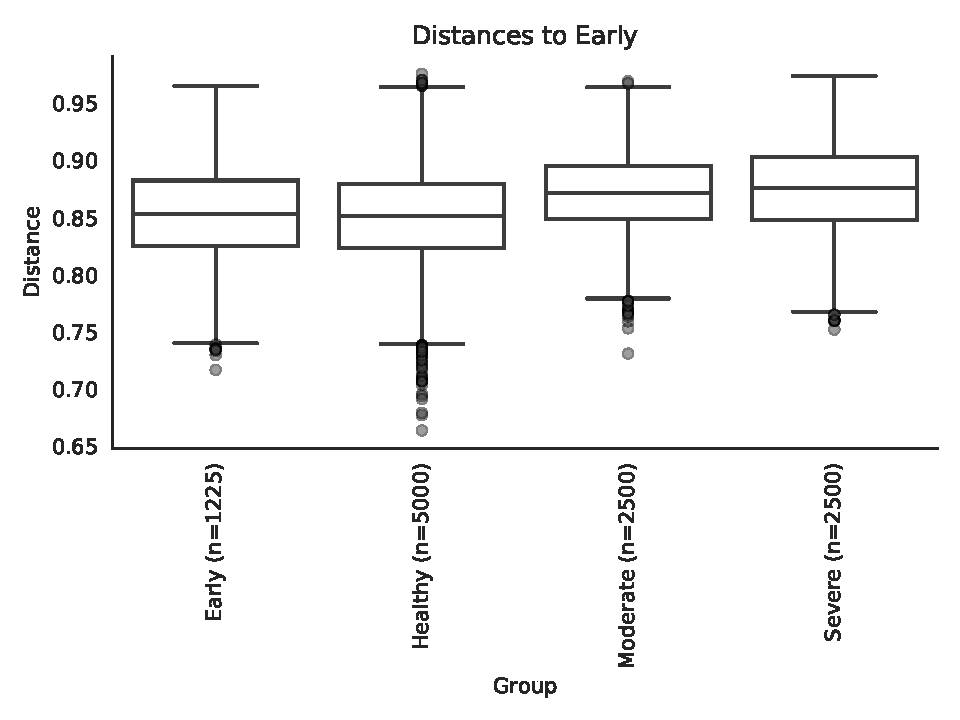
\includegraphics[width=0.4 \linewidth]{figures/BetaDiversity/DADA2/Jaccard/Early.pdf}
                    \\
                    \mbox{(a) Healthy} & \mbox{(b) Early} \\

                    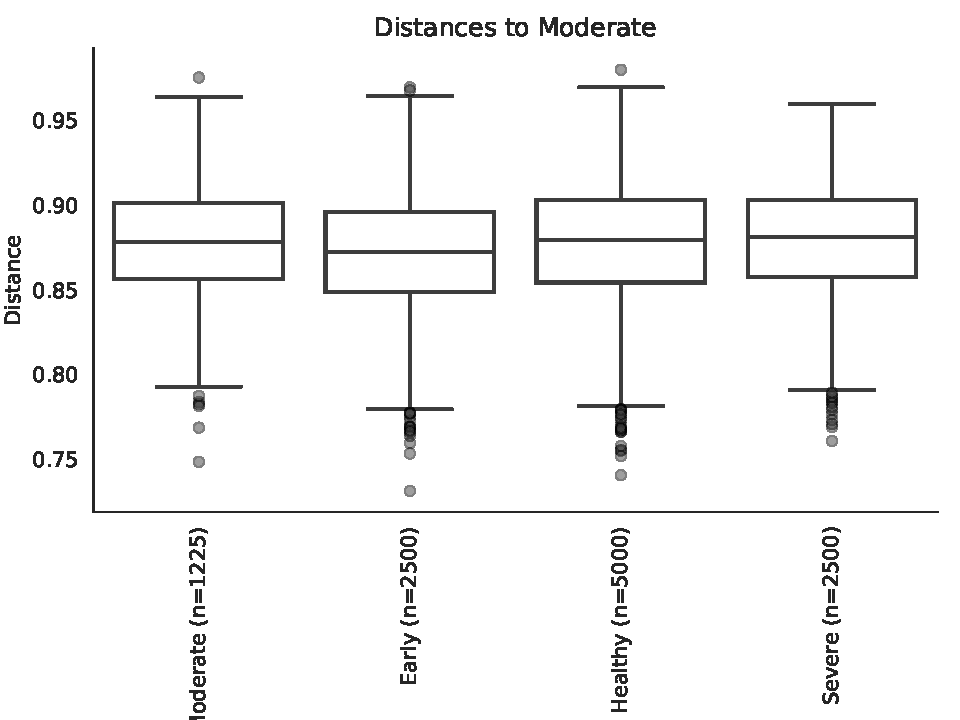
\includegraphics[width=0.4 \linewidth]{figures/BetaDiversity/DADA2/Jaccard/Moderate.pdf}
                    &
                    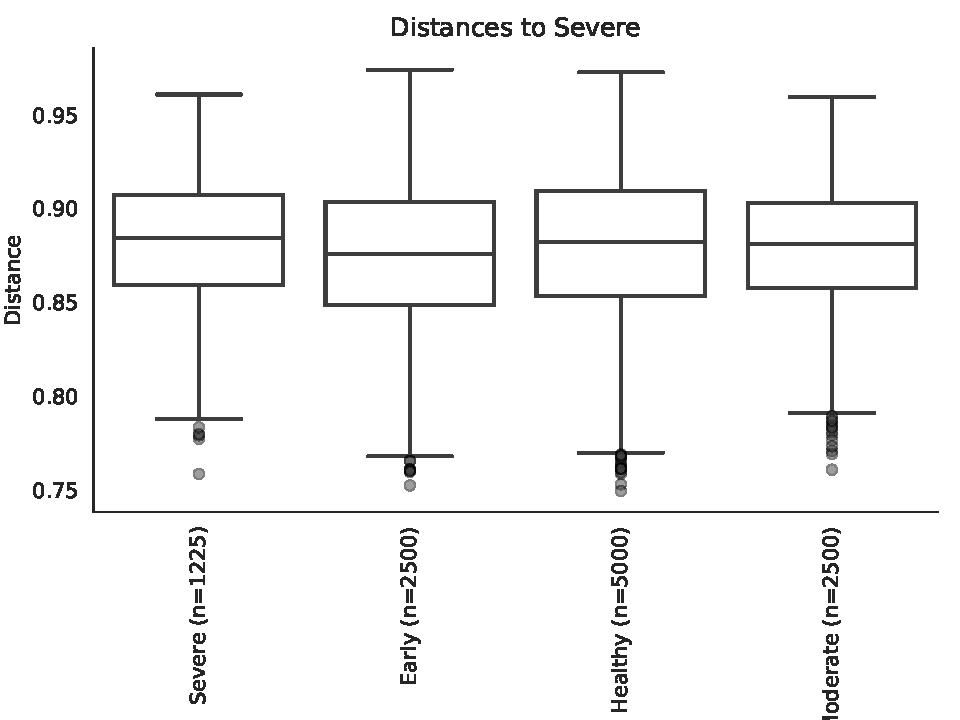
\includegraphics[width=0.4 \linewidth]{figures/BetaDiversity/DADA2/Jaccard/Severe.pdf}
                    \\
                    \mbox{(c) Moderate} & \mbox{(d) Severe} \\
                \end{array}$
                \caption{Jaccard Distance Index with DADA2}
                \label{fig:jaccard-dada2}
            \end{figure}

            \begin{figure}[p]
                \centering
                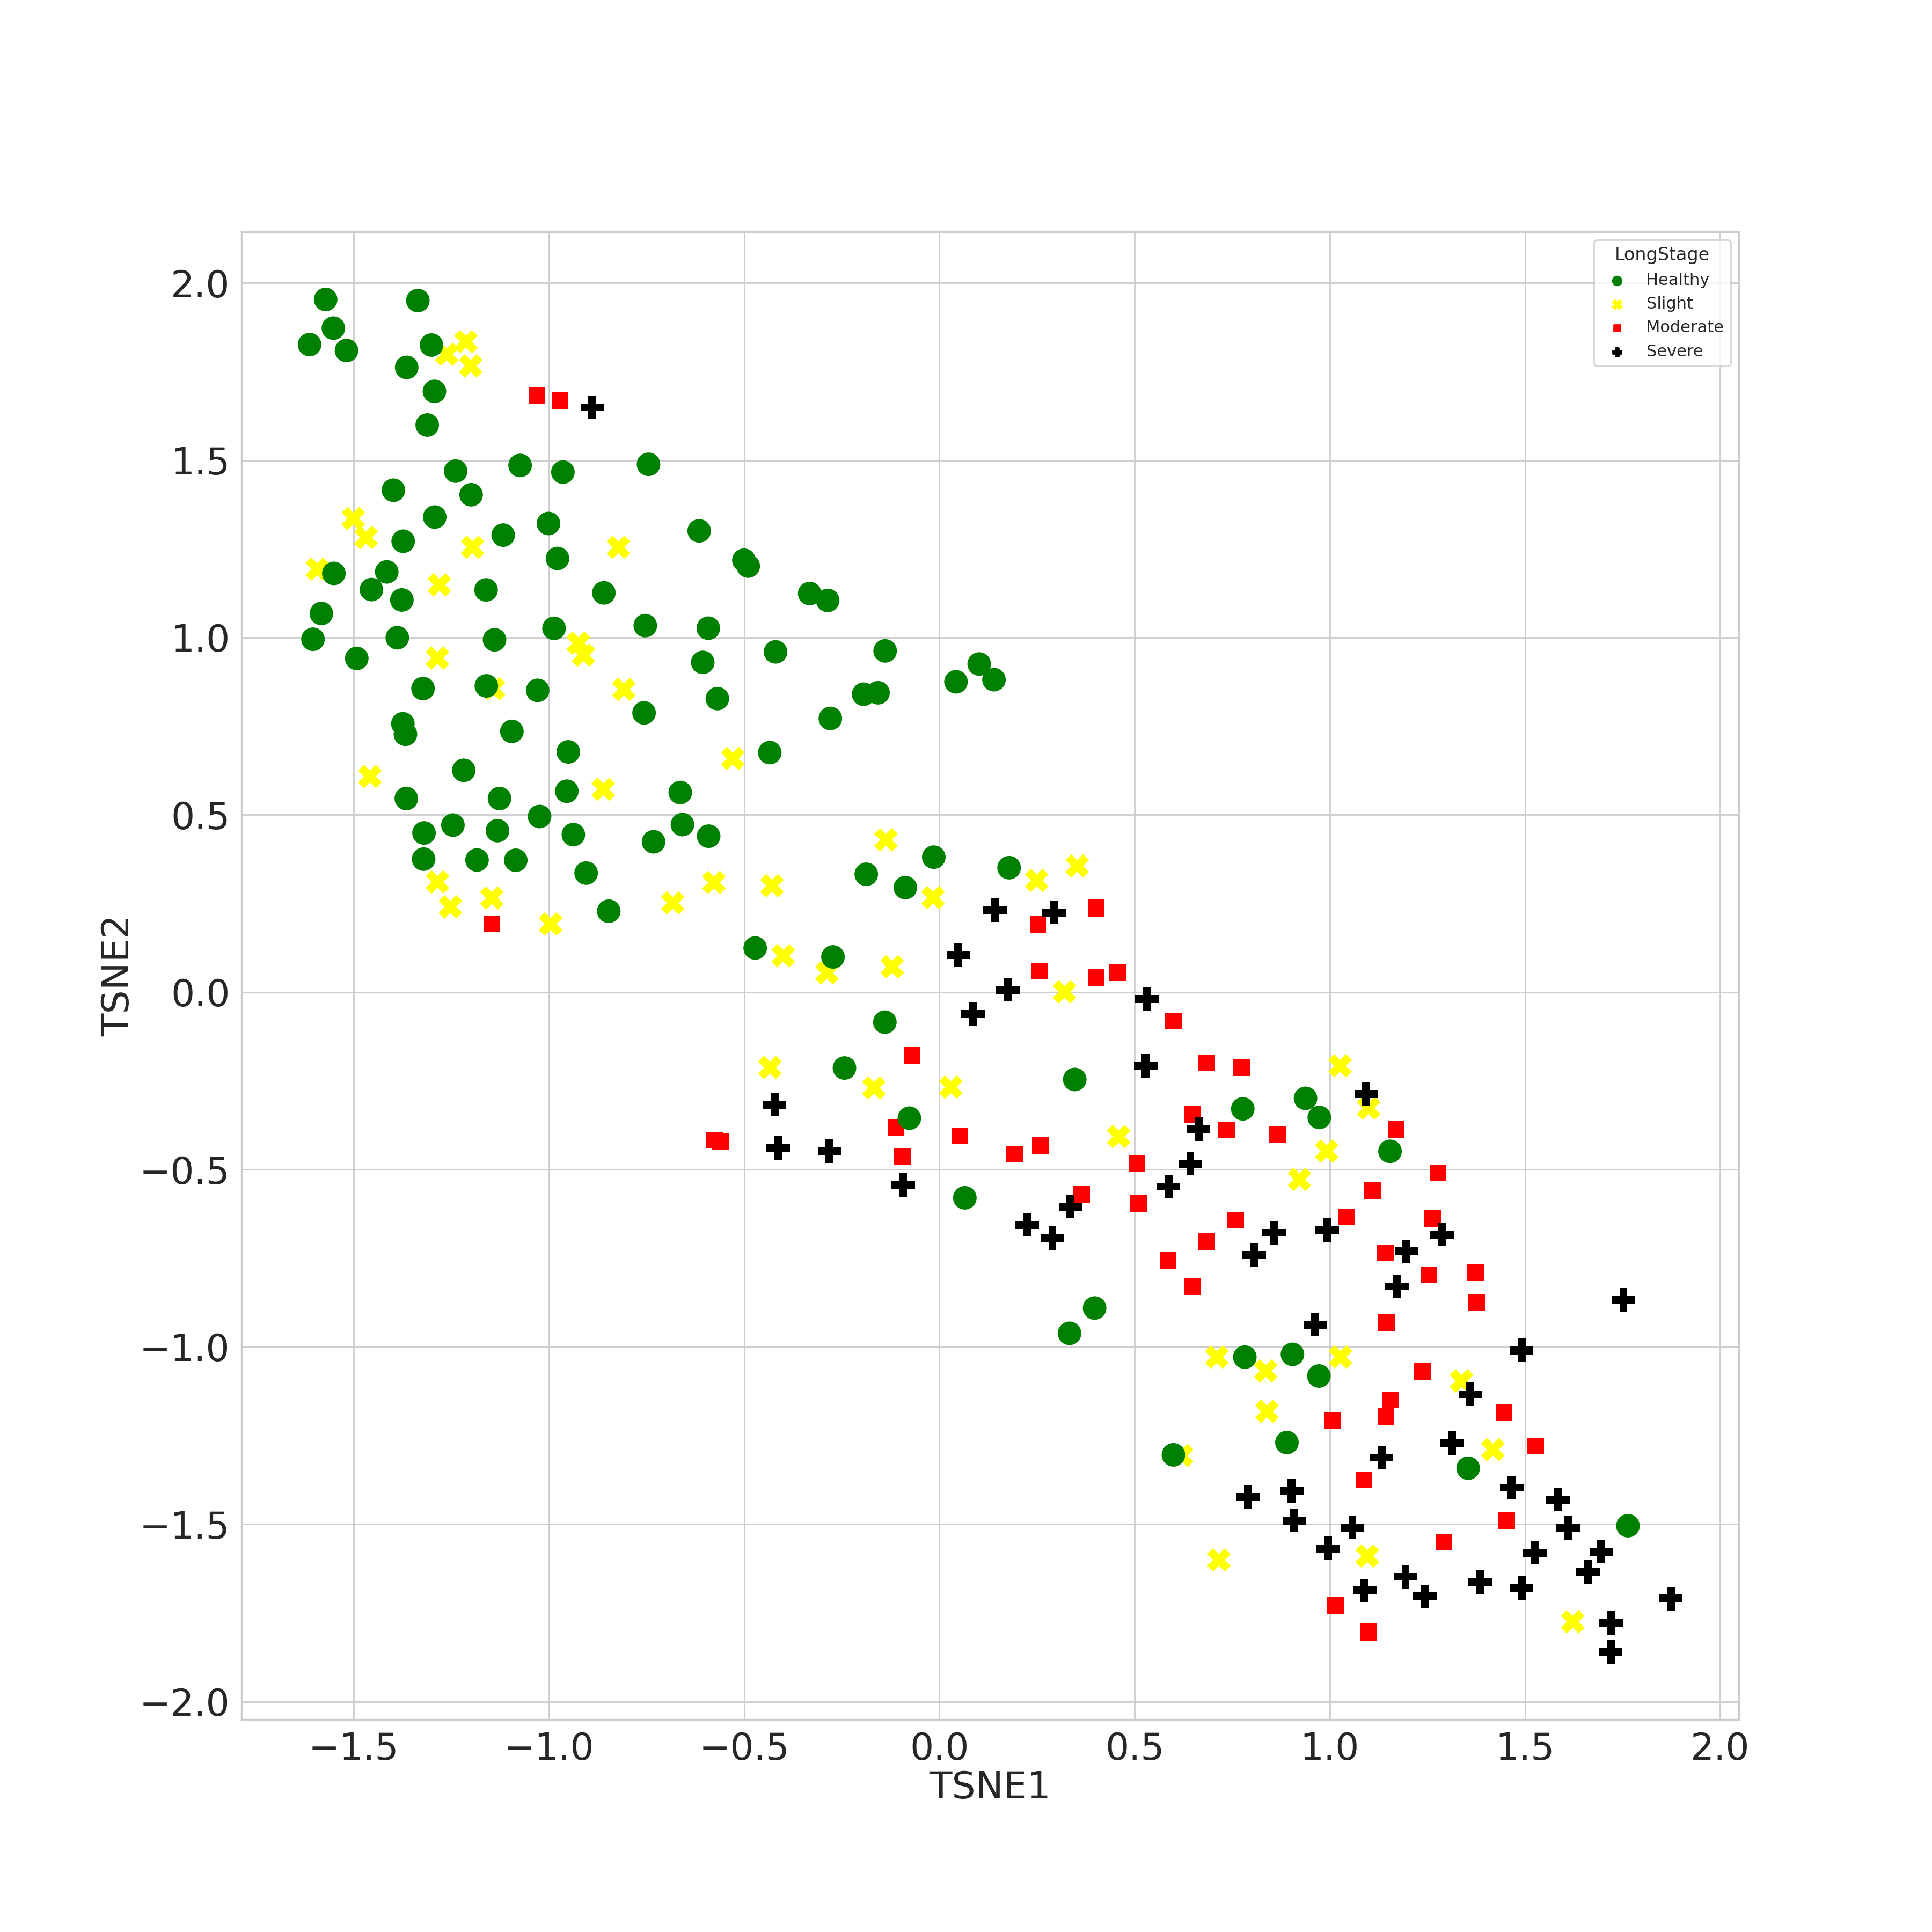
\includegraphics[width=0.6 \linewidth]{figures/BetaDiversity/DADA2.unweighted_unifrac.png}
                \caption{t-SNE Plot from Unweighted UniFrac Distance Index with DADA2}
                \label{fig:tsne-unweighted-dada2}
            \end{figure}

            \begin{figure}[p]
                \centering
                $\begin{array}{cc}
                    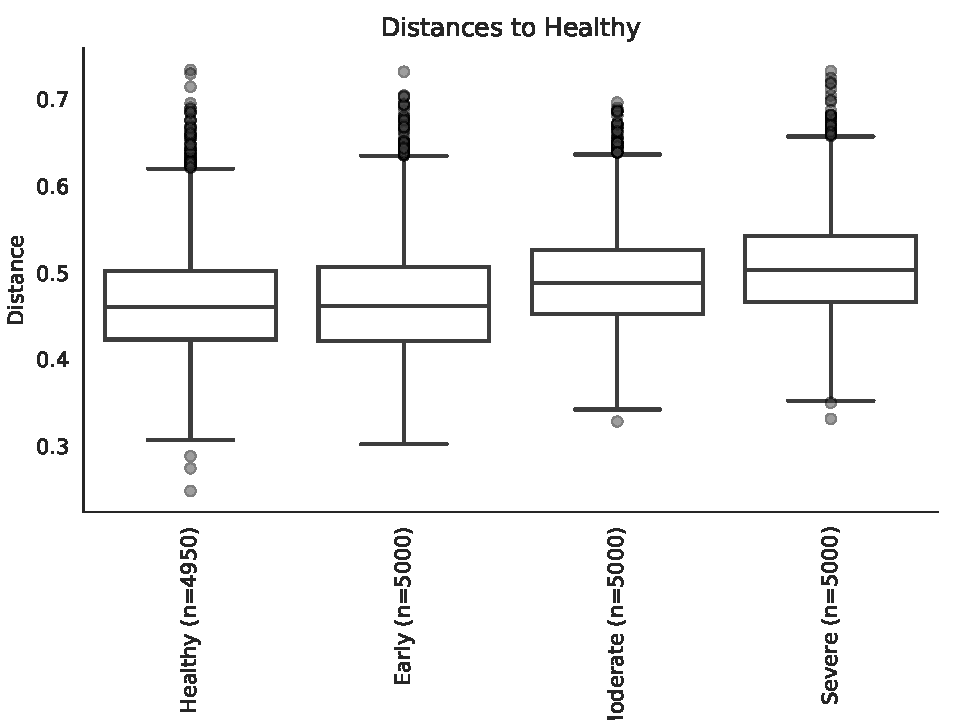
\includegraphics[width=0.4 \linewidth]{figures/BetaDiversity/DADA2/UnweightedUnifrac/Healthy.pdf}
                    &
                    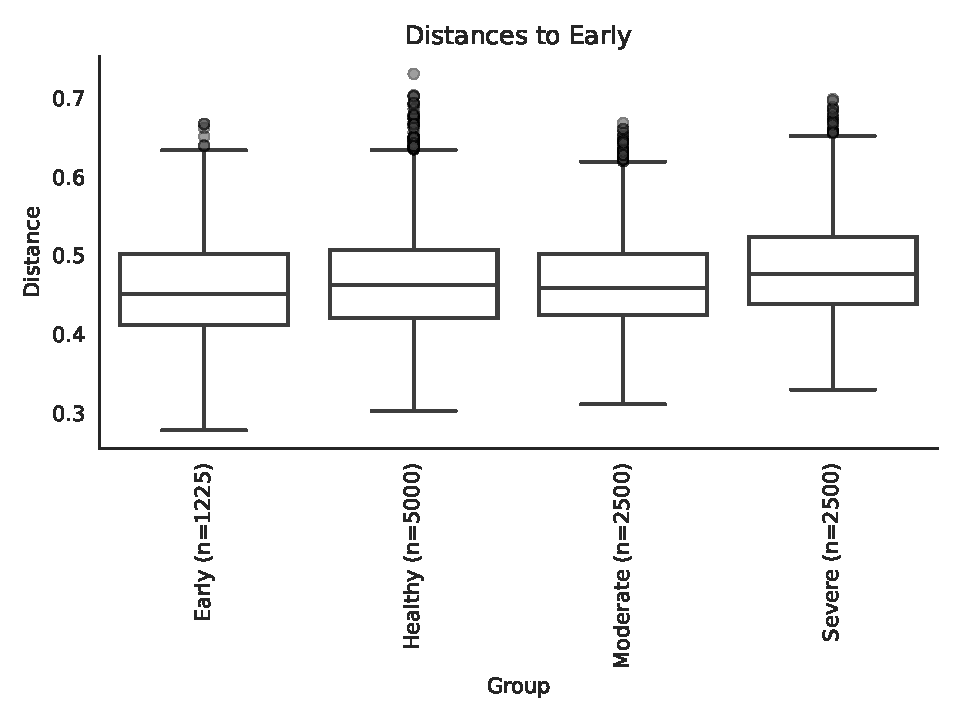
\includegraphics[width=0.4 \linewidth]{figures/BetaDiversity/DADA2/UnweightedUnifrac/Early.pdf}
                    \\
                    \mbox{(a) Healthy} & \mbox{(b) Early} \\

                    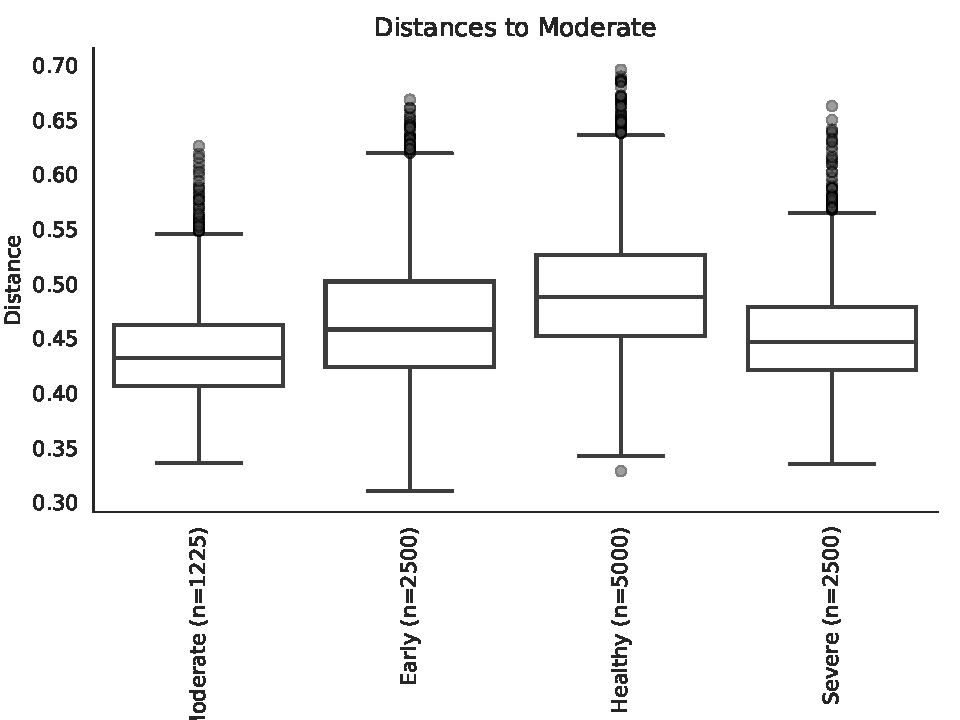
\includegraphics[width=0.4 \linewidth]{figures/BetaDiversity/DADA2/UnweightedUnifrac/Moderate.pdf}
                    &
                    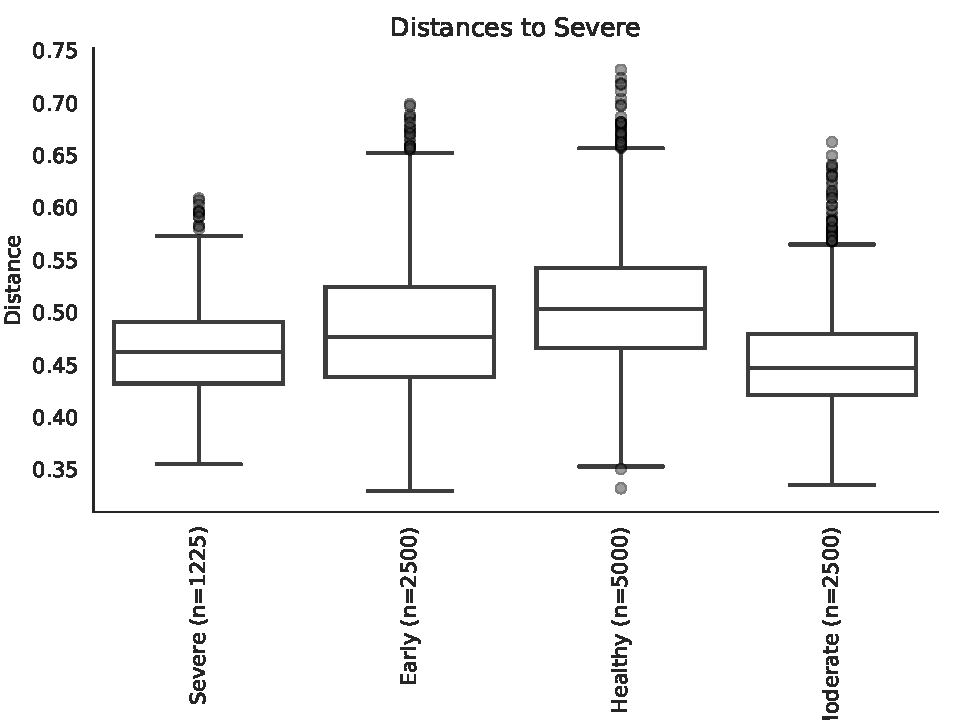
\includegraphics[width=0.4 \linewidth]{figures/BetaDiversity/DADA2/UnweightedUnifrac/Severe.pdf}
                    \\
                    \mbox{(c) Moderate} & \mbox{(d) Severe} \\
                \end{array}$
                \caption{Unweighted UniFrac Distance Index with DADA2}
                \label{fig:unweighted-dada2}
            \end{figure}

            \begin{figure}[p]
                \centering
                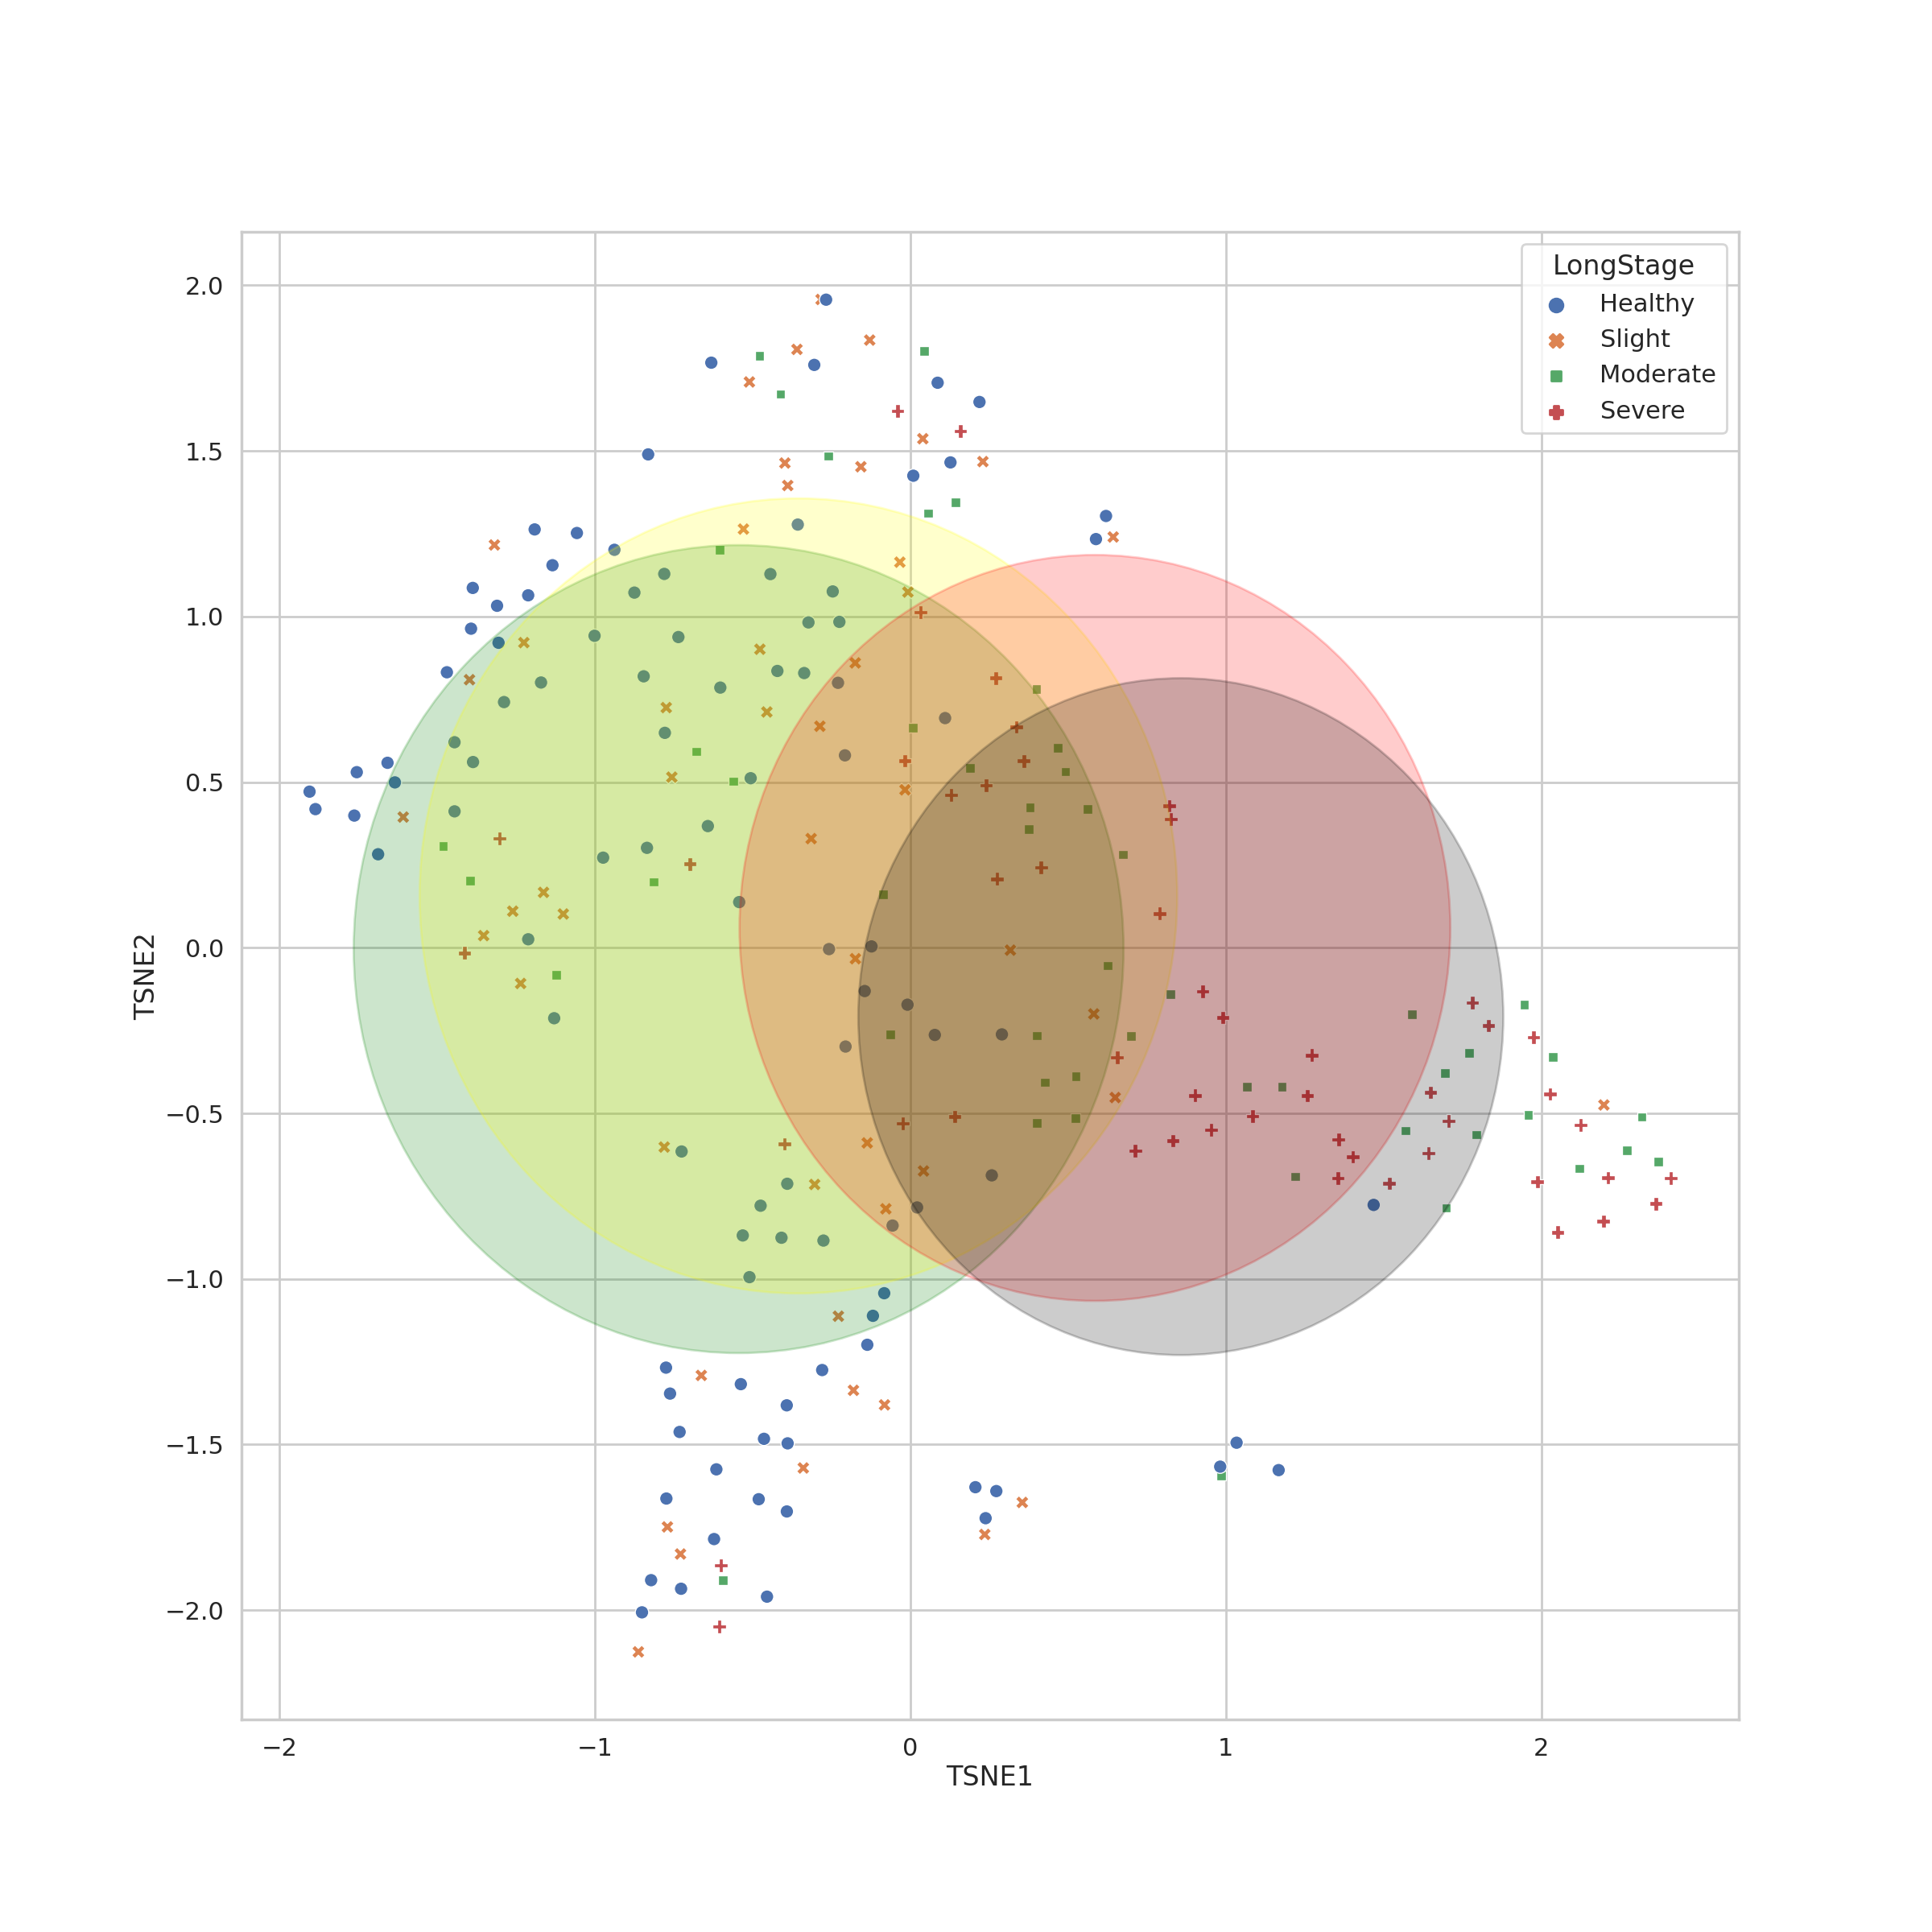
\includegraphics[width=0.6 \linewidth]{figures/BetaDiversity/DADA2.weighted_unifrac.png}
                \caption{t-SNE Plot from Weighted UniFrac Distance Index with DADA2}
                \label{fig:tsne-weighted-dada2}
            \end{figure}

            \begin{figure}[p]
                \centering
                $\begin{array}{cc}
                    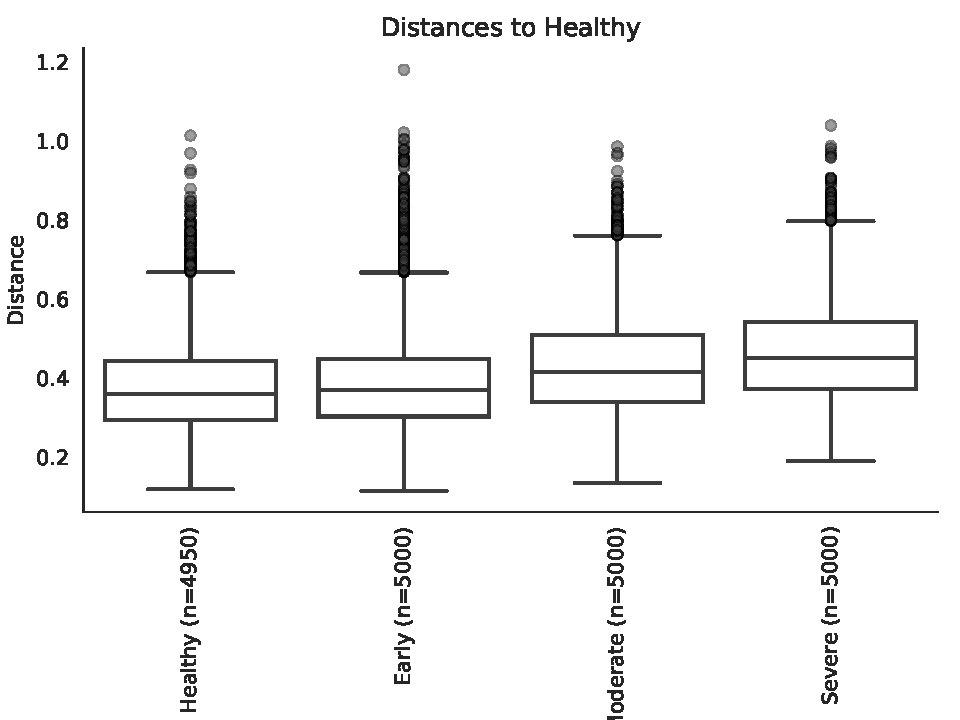
\includegraphics[width=0.4 \linewidth]{figures/BetaDiversity/DADA2/WeightedUnifrac/Healthy.pdf}
                    &
                    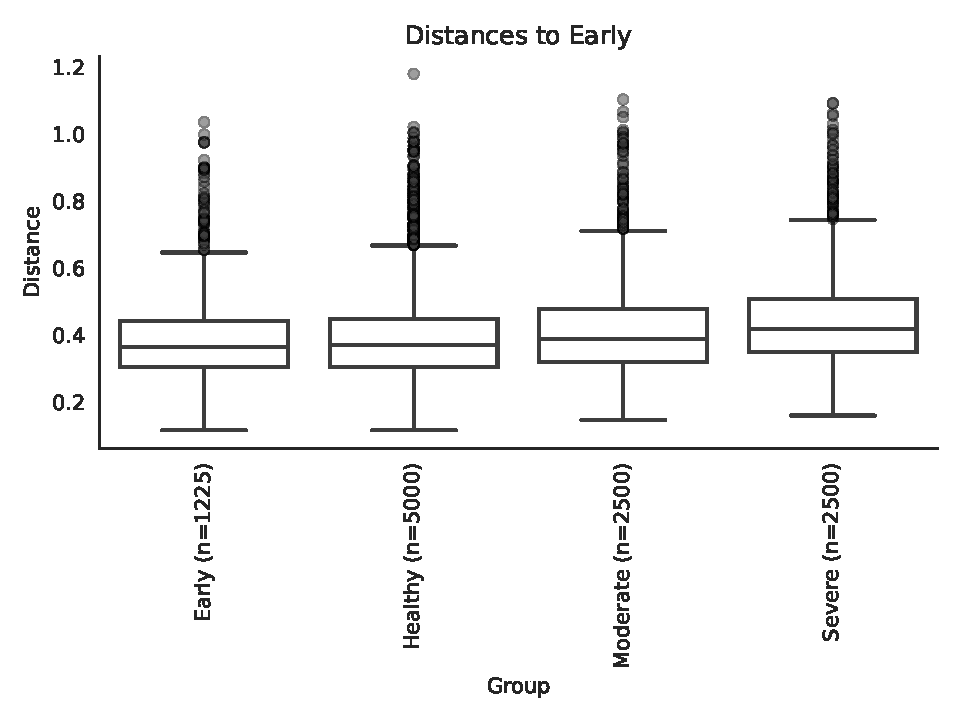
\includegraphics[width=0.4 \linewidth]{figures/BetaDiversity/DADA2/WeightedUnifrac/Early.pdf}
                    \\
                    \mbox{(a) Healthy} & \mbox{(b) Early} \\

                    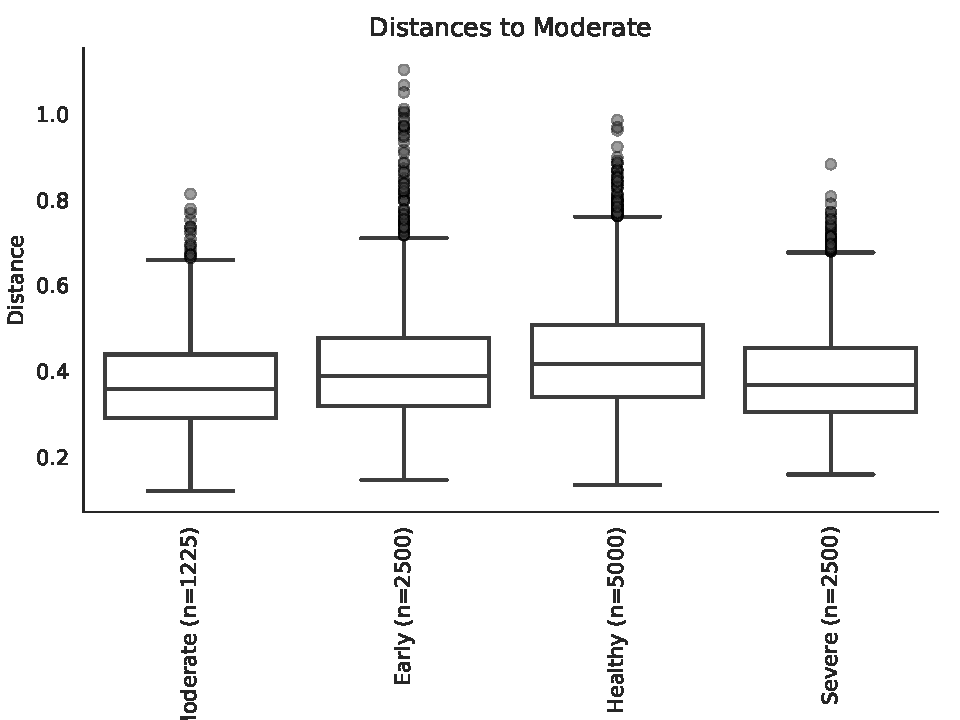
\includegraphics[width=0.4 \linewidth]{figures/BetaDiversity/DADA2/WeightedUnifrac/Moderate.pdf}
                    &
                    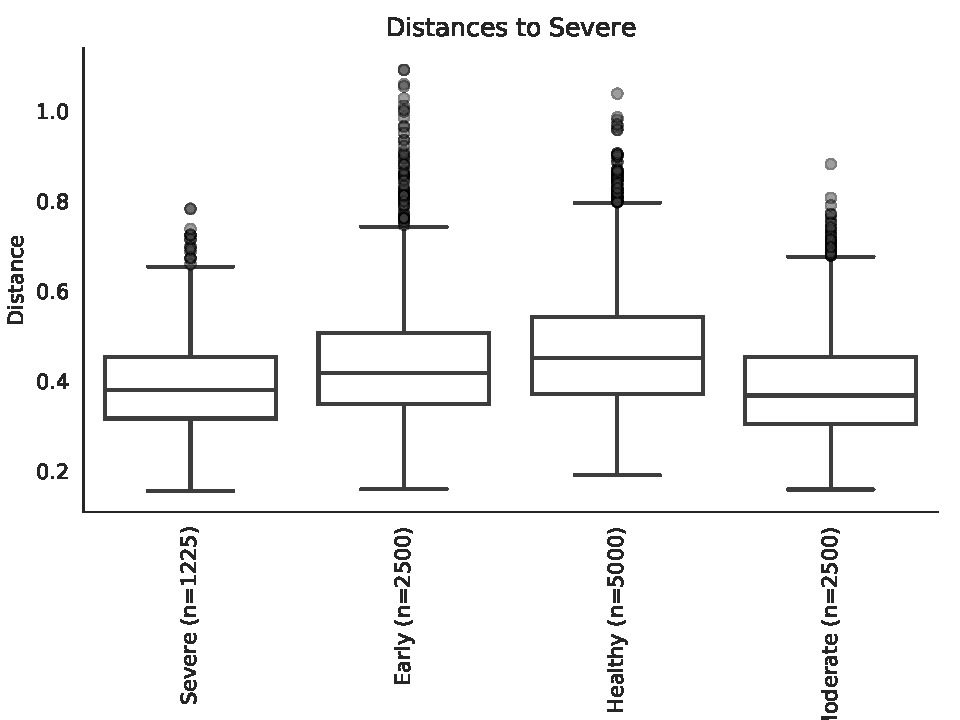
\includegraphics[width=0.4 \linewidth]{figures/BetaDiversity/DADA2/WeightedUnifrac/Severe.pdf}
                    \\
                    \mbox{(c) Moderate} & \mbox{(d) Severe} \\
                \end{array}$
                \caption{Weighted UniFrac Distance Index with DADA2}
                \label{fig:weighted-dada2}
            \end{figure}

        \subsection{ANCOM}

            \begin{table}[p]
                \centering
                \caption{ANCOM Significant Taxa with DADA2 and HOMD}
                \label{tb:ANCOM-dada2-gg}

                \csvreader[tabular=p{10cm}cc, no head, column count=3, table head=\hline, late after first line=\\\hline, table foot=\hline, respect underscore]{csv/ANCOM/DADA2.homd.csv}{}{\csvlinetotablerow}
            \end{table}

            \begin{figure}[p]
                \centering
                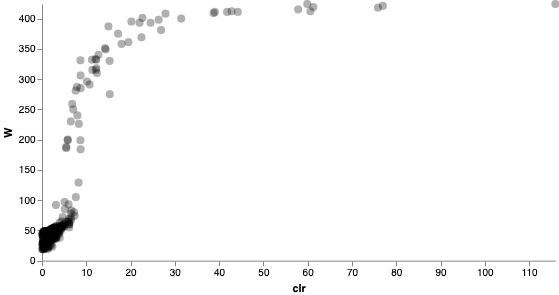
\includegraphics[width=0.8 \linewidth]{figures/ANCOM/DADA2.homd.png}
                \caption{ANCOM Volcano Plot with DADA2 and GG}
                \label{fig:volcano-dada2-gg}
            \end{figure}

        \subsection{t-SNE Plot with Whole Microbiome}
            As mentioned herein-before, t-SNE is a technique which reduce multi-dimensional data into two-dimension. Whole microbiome data are multi-dimensional data, which have \textit{circa} 600 columns, so the data should be reduced their dimension for readability. Hence, by the grace of t-SNE, the microbiome data have been deflated their dimension: 328 taxa from DADA2 and GG (Figure \ref{fig:tsne-whole-dada2-gg}), 633 taxa from DADA2 and SILVA (Figure \ref{fig:tsne-whole-dada2-silva}), 425 taxa from DADA2 and HOMD (Figure \ref{fig:tsne-whole-dada2-homd}), 232 taxa from Deblur and GG (Figure \ref{fig:tsne-whole-deblur-gg}), 414 taxa from Deblur and SILVA (Figure \ref{fig:tsne-whole-deblur-silva}) and 235 taxa from Deblur and HOMD (Figure \ref{fig:tsne-whole-deblur-homd}).

            \begin{figure}[p]
                \centering
                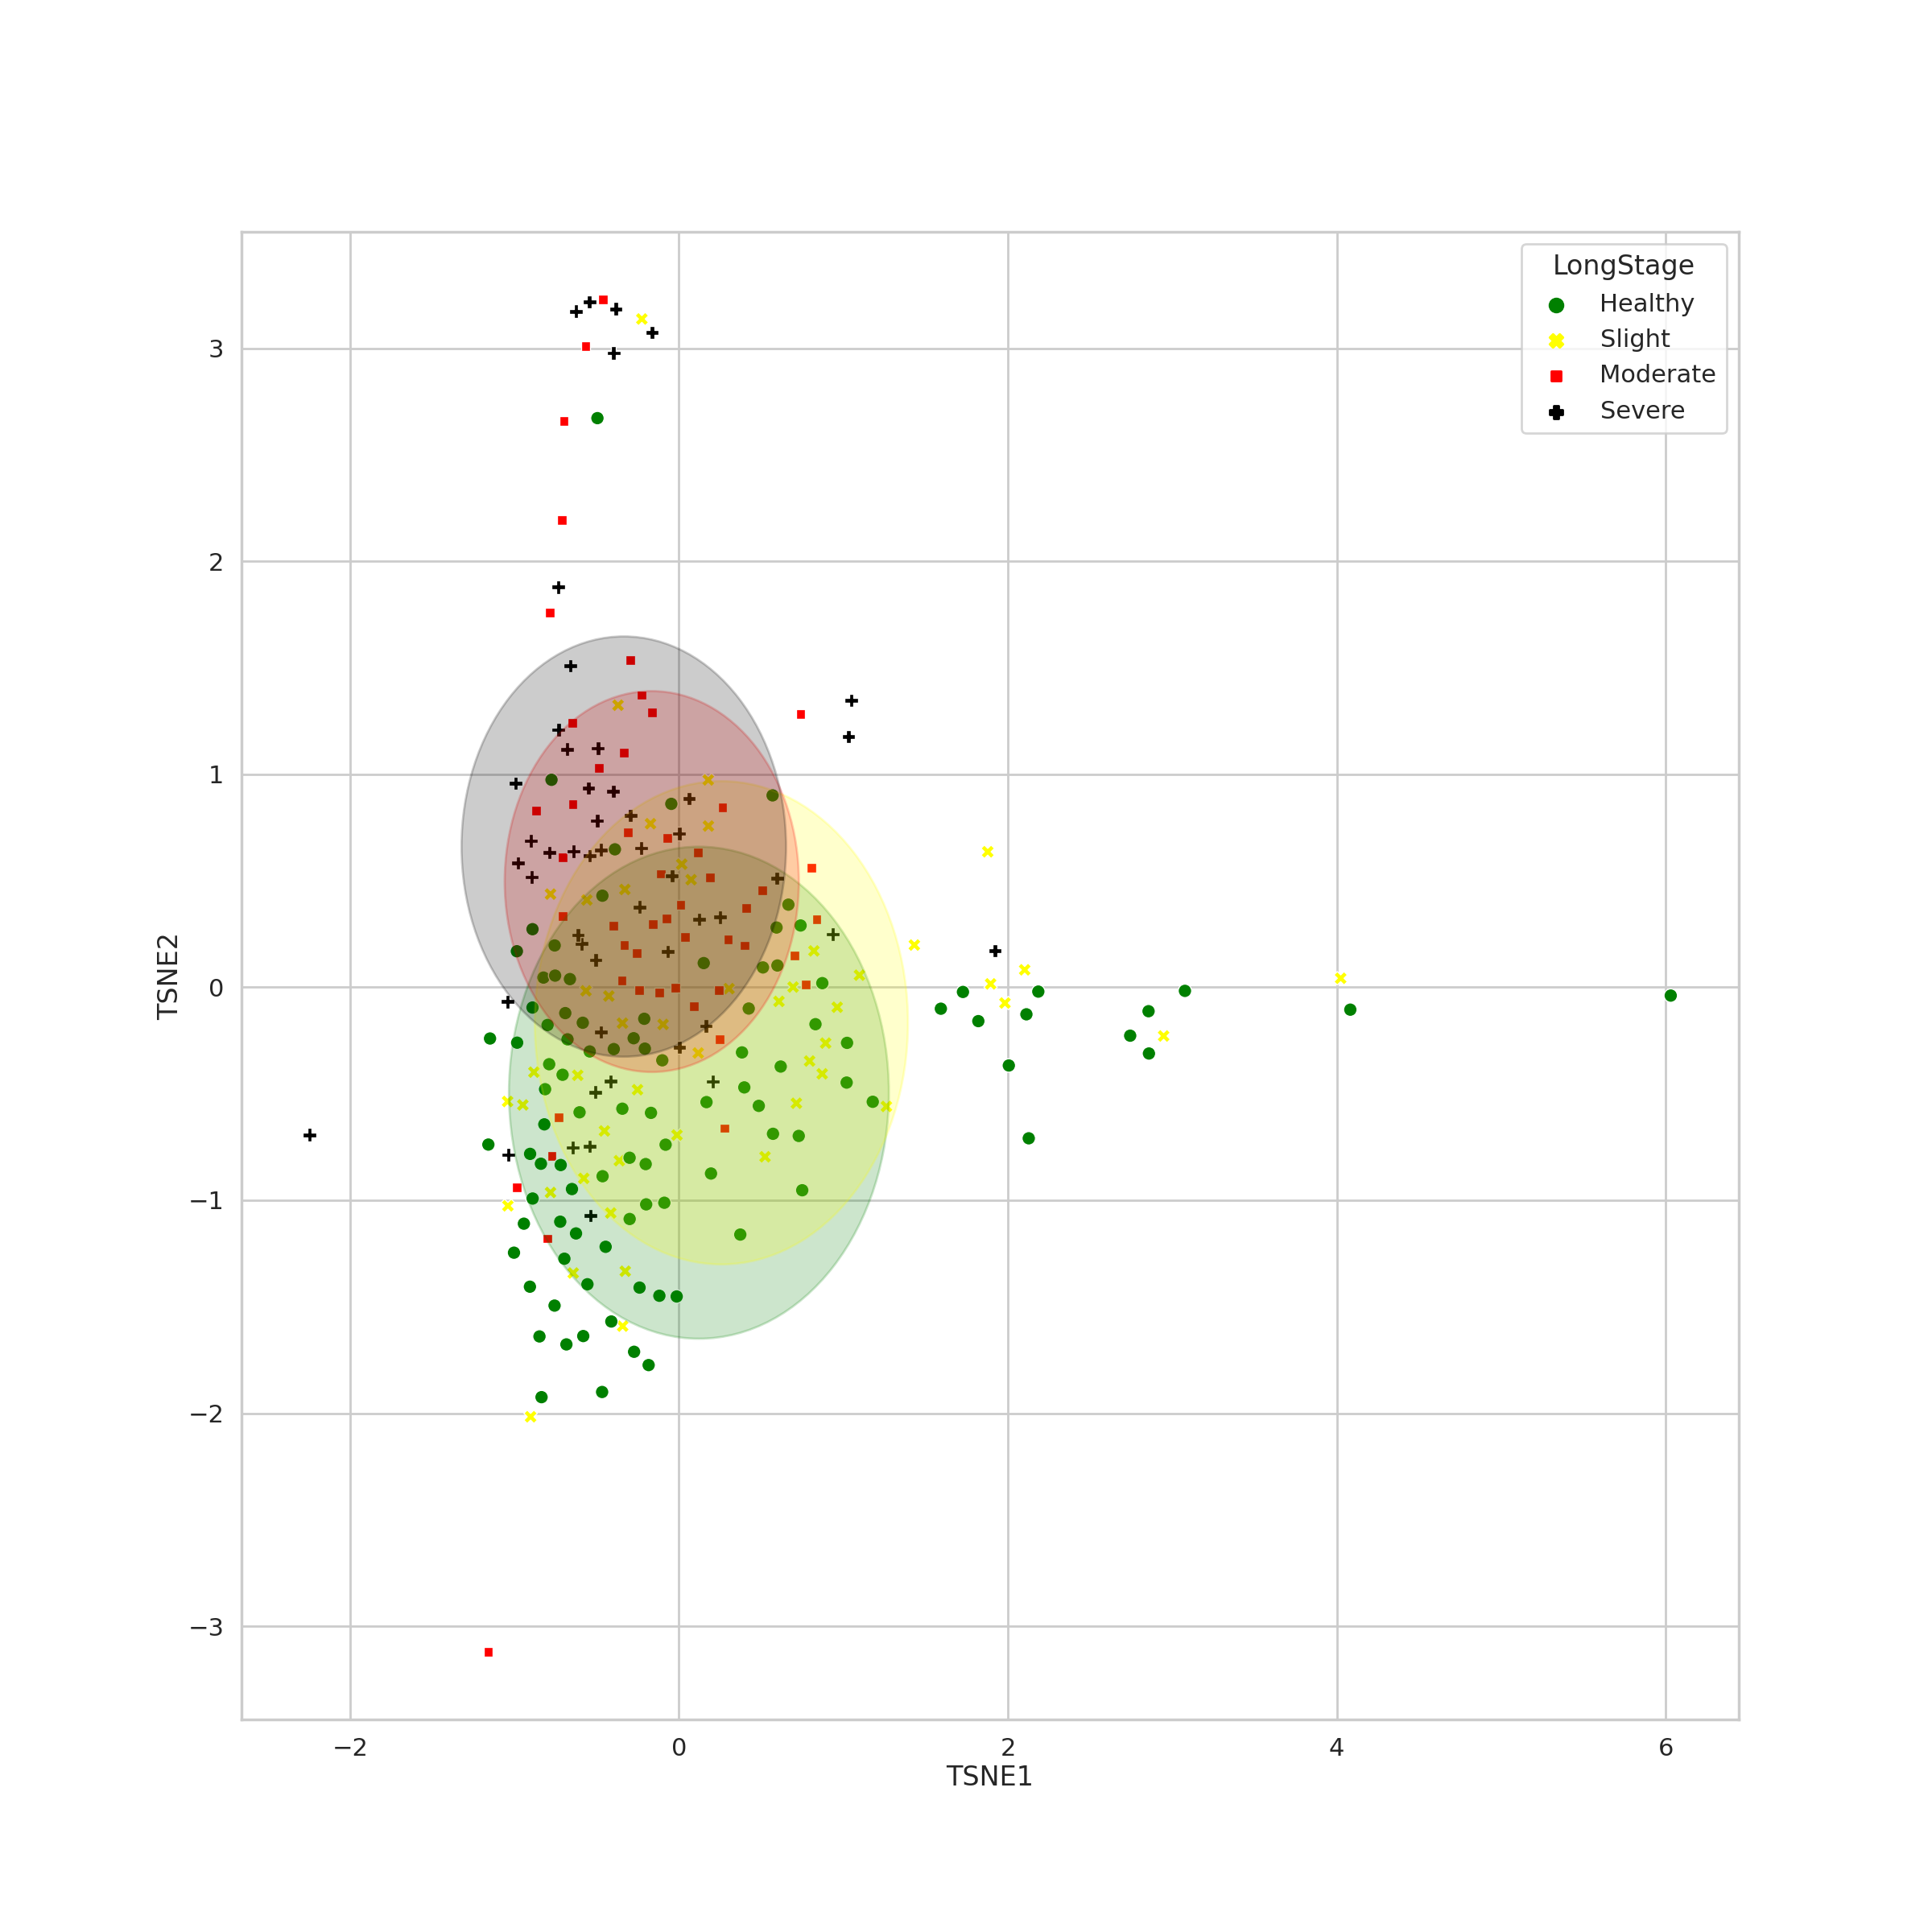
\includegraphics[width=0.6 \linewidth]{figures/tSNE/Whole/whole.DADA2.gg.png}
                \caption{t-SNE Plot with Whole Microbiome from DADA2 and GG (328 taxa)}
                \label{fig:tsne-whole-dada2-gg}
            \end{figure}

            \begin{figure}[p]
                \centering
                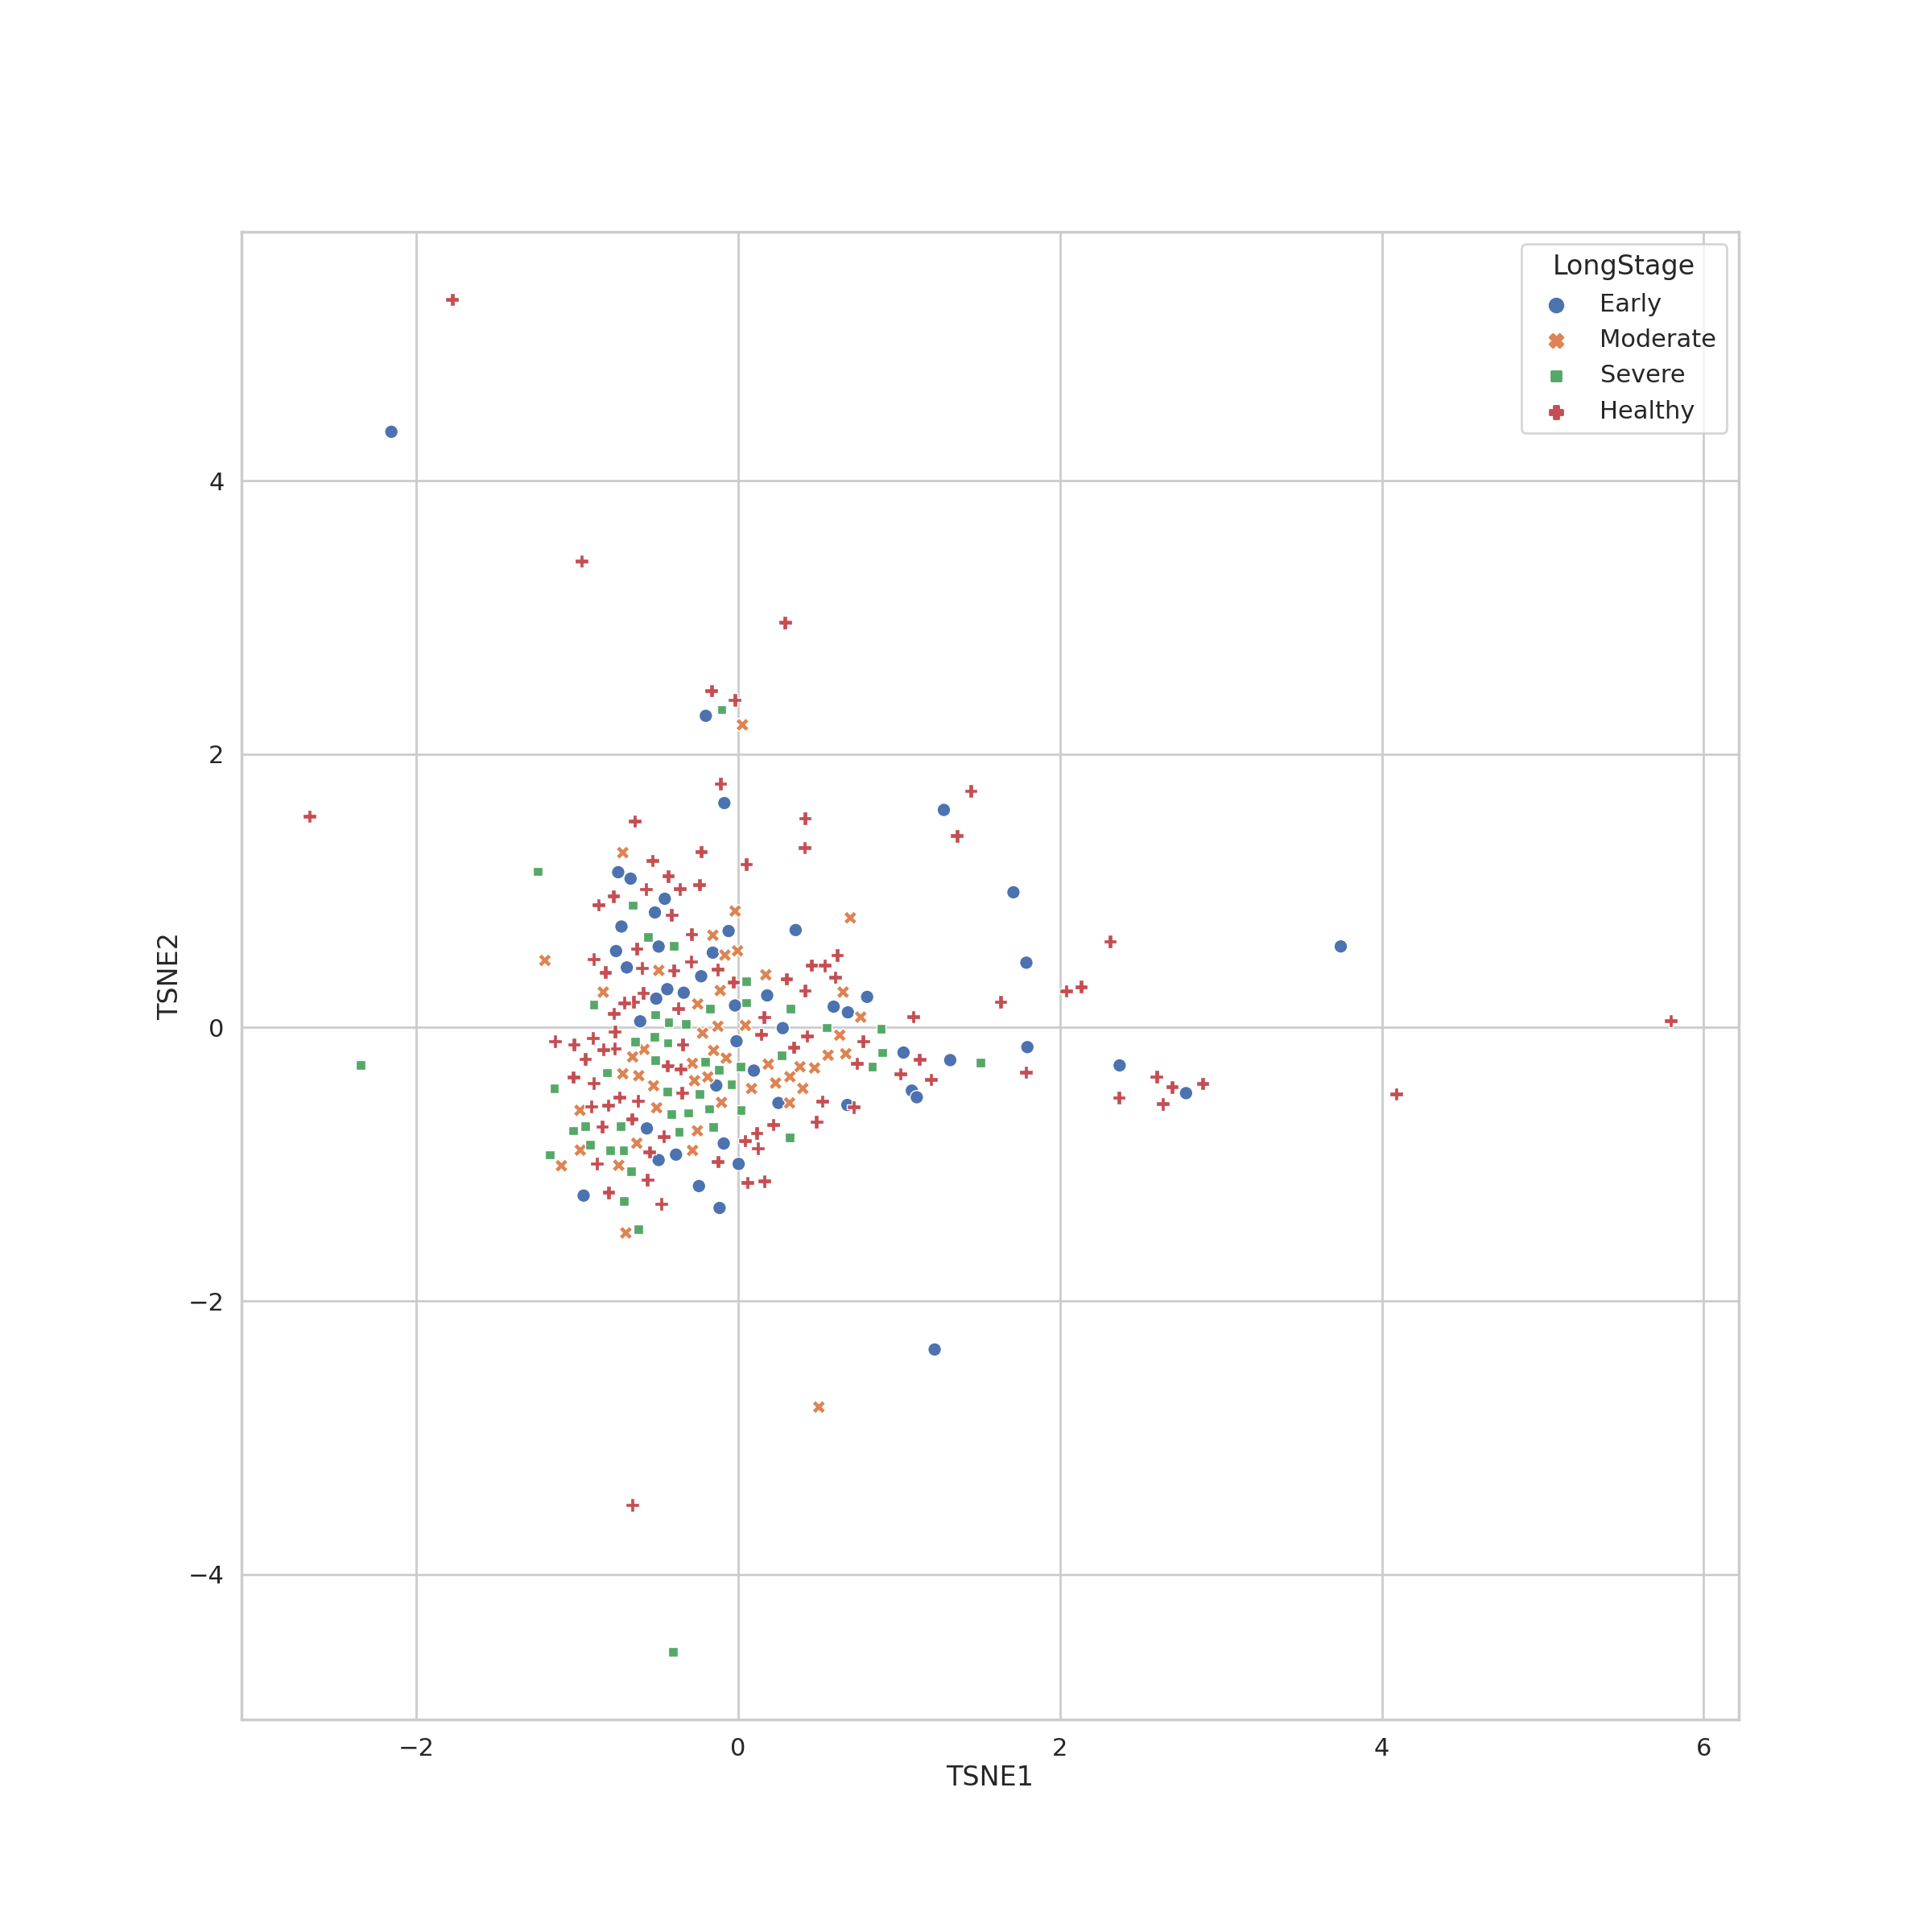
\includegraphics[width=0.6 \linewidth]{figures/tSNE/Whole/whole.DADA2.silva.png}
                \caption{t-SNE Plot with Whole Microbiome from DADA2 and SILVA (633 taxa)}
                \label{fig:tsne-whole-dada2-silva}
            \end{figure}

            \begin{figure}[p]
                \centering
                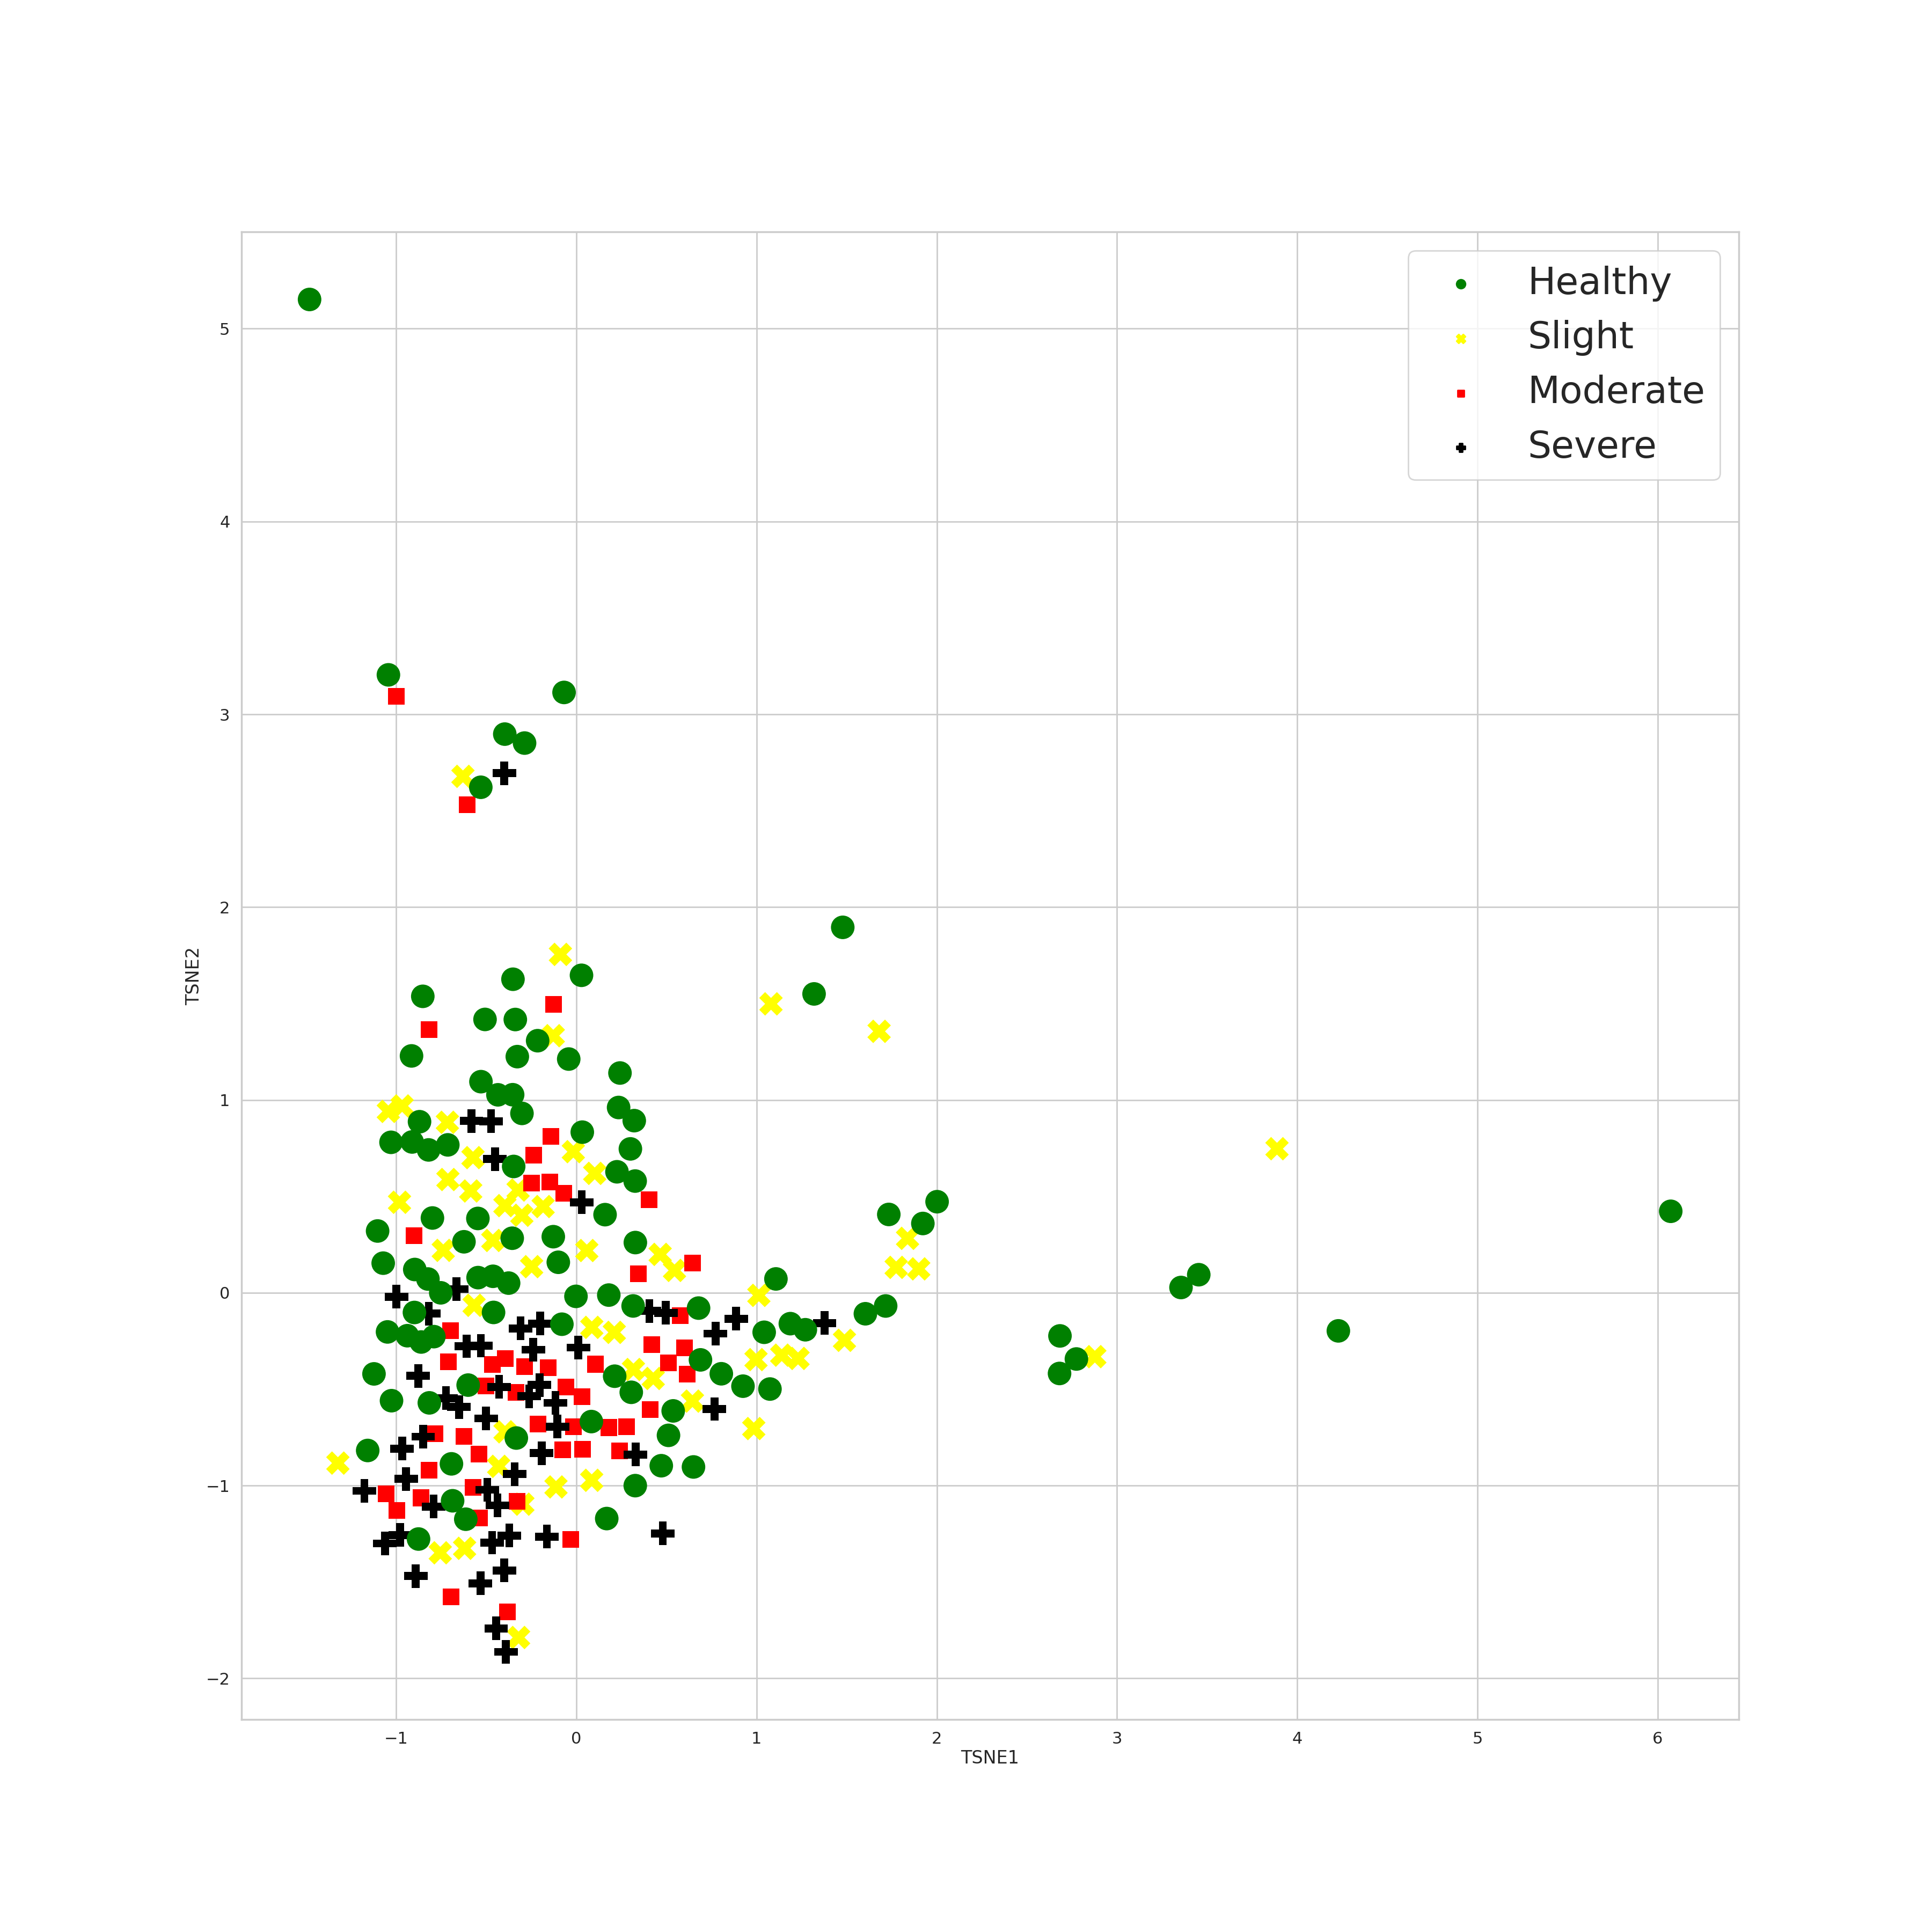
\includegraphics[width=0.6 \linewidth]{figures/tSNE/Whole/whole.DADA2.homd.png}
                \caption{t-SNE Plot with Whole Microbiome from DADA2 and HOMD (425 taxa)}
                \label{fig:tsne-whole-dada2-homd}
            \end{figure}

            \begin{figure}[p]
                \centering
                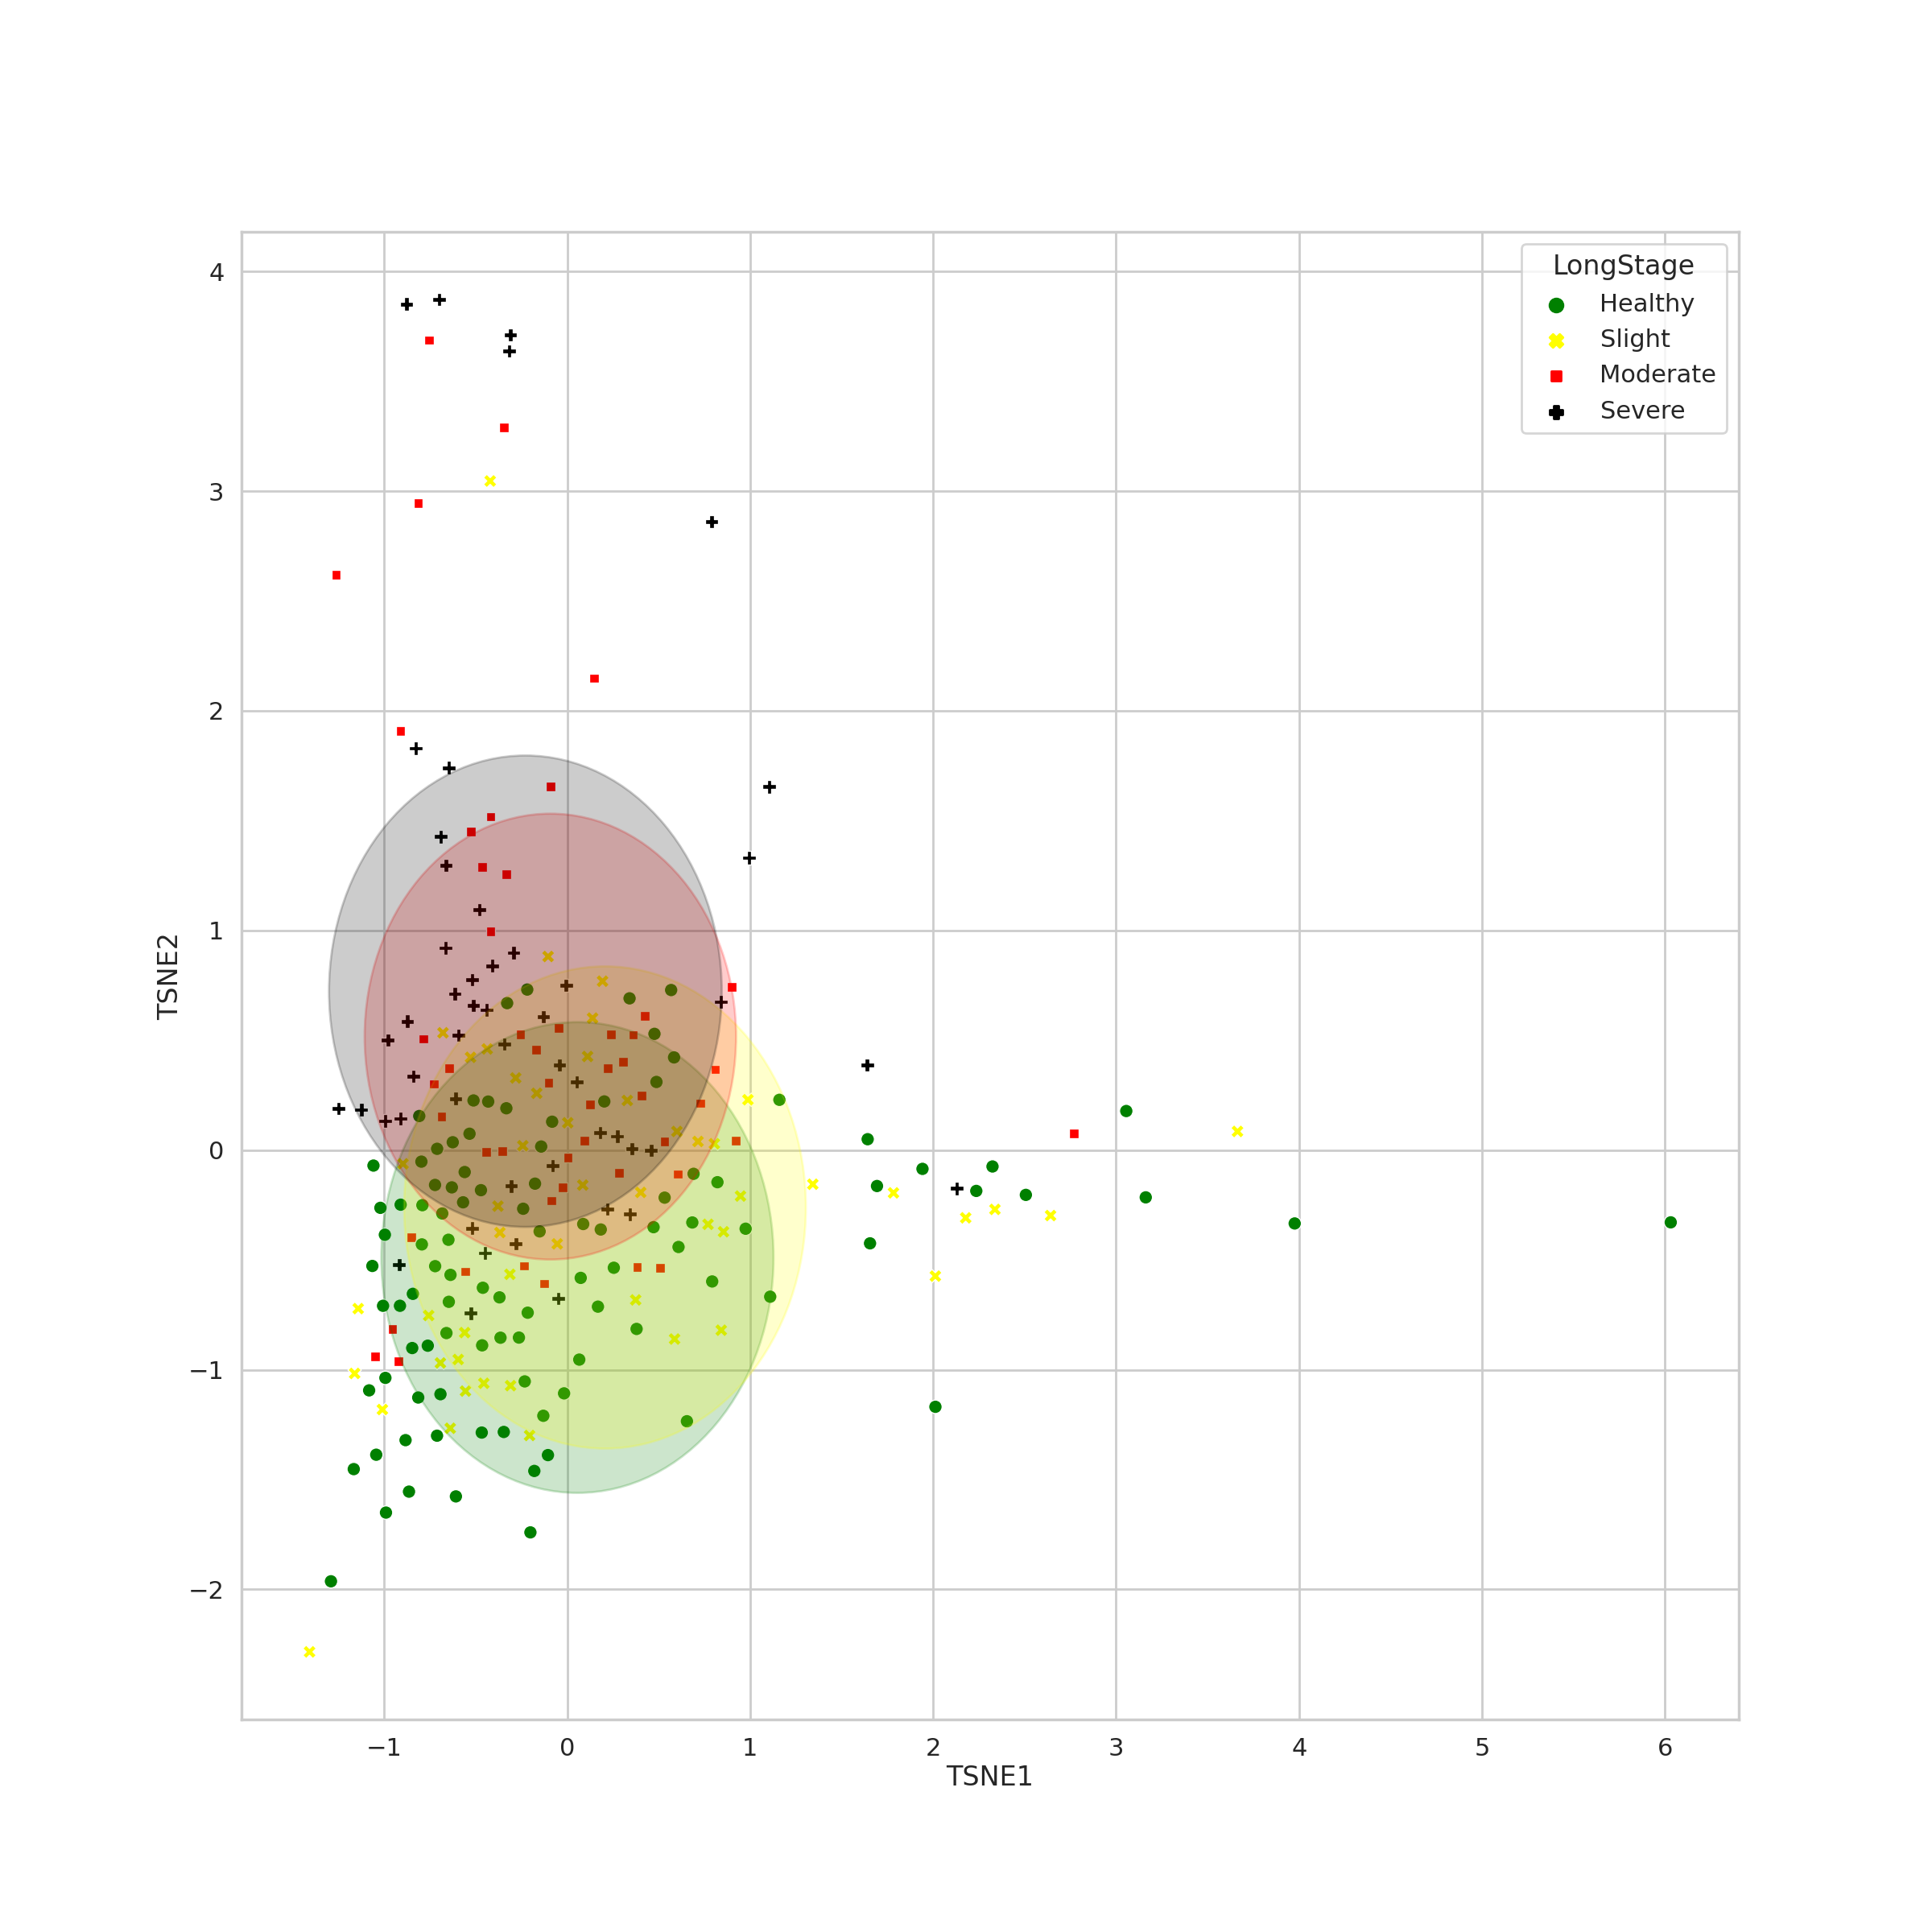
\includegraphics[width=0.6 \linewidth]{figures/tSNE/Whole/whole.Deblur.gg.png}
                \caption{t-SNE Plot with Whole Microbiome from Deblur and GG (232 taxa)}
                \label{fig:tsne-whole-deblur-gg}
            \end{figure}

            \begin{figure}[p]
                \centering
                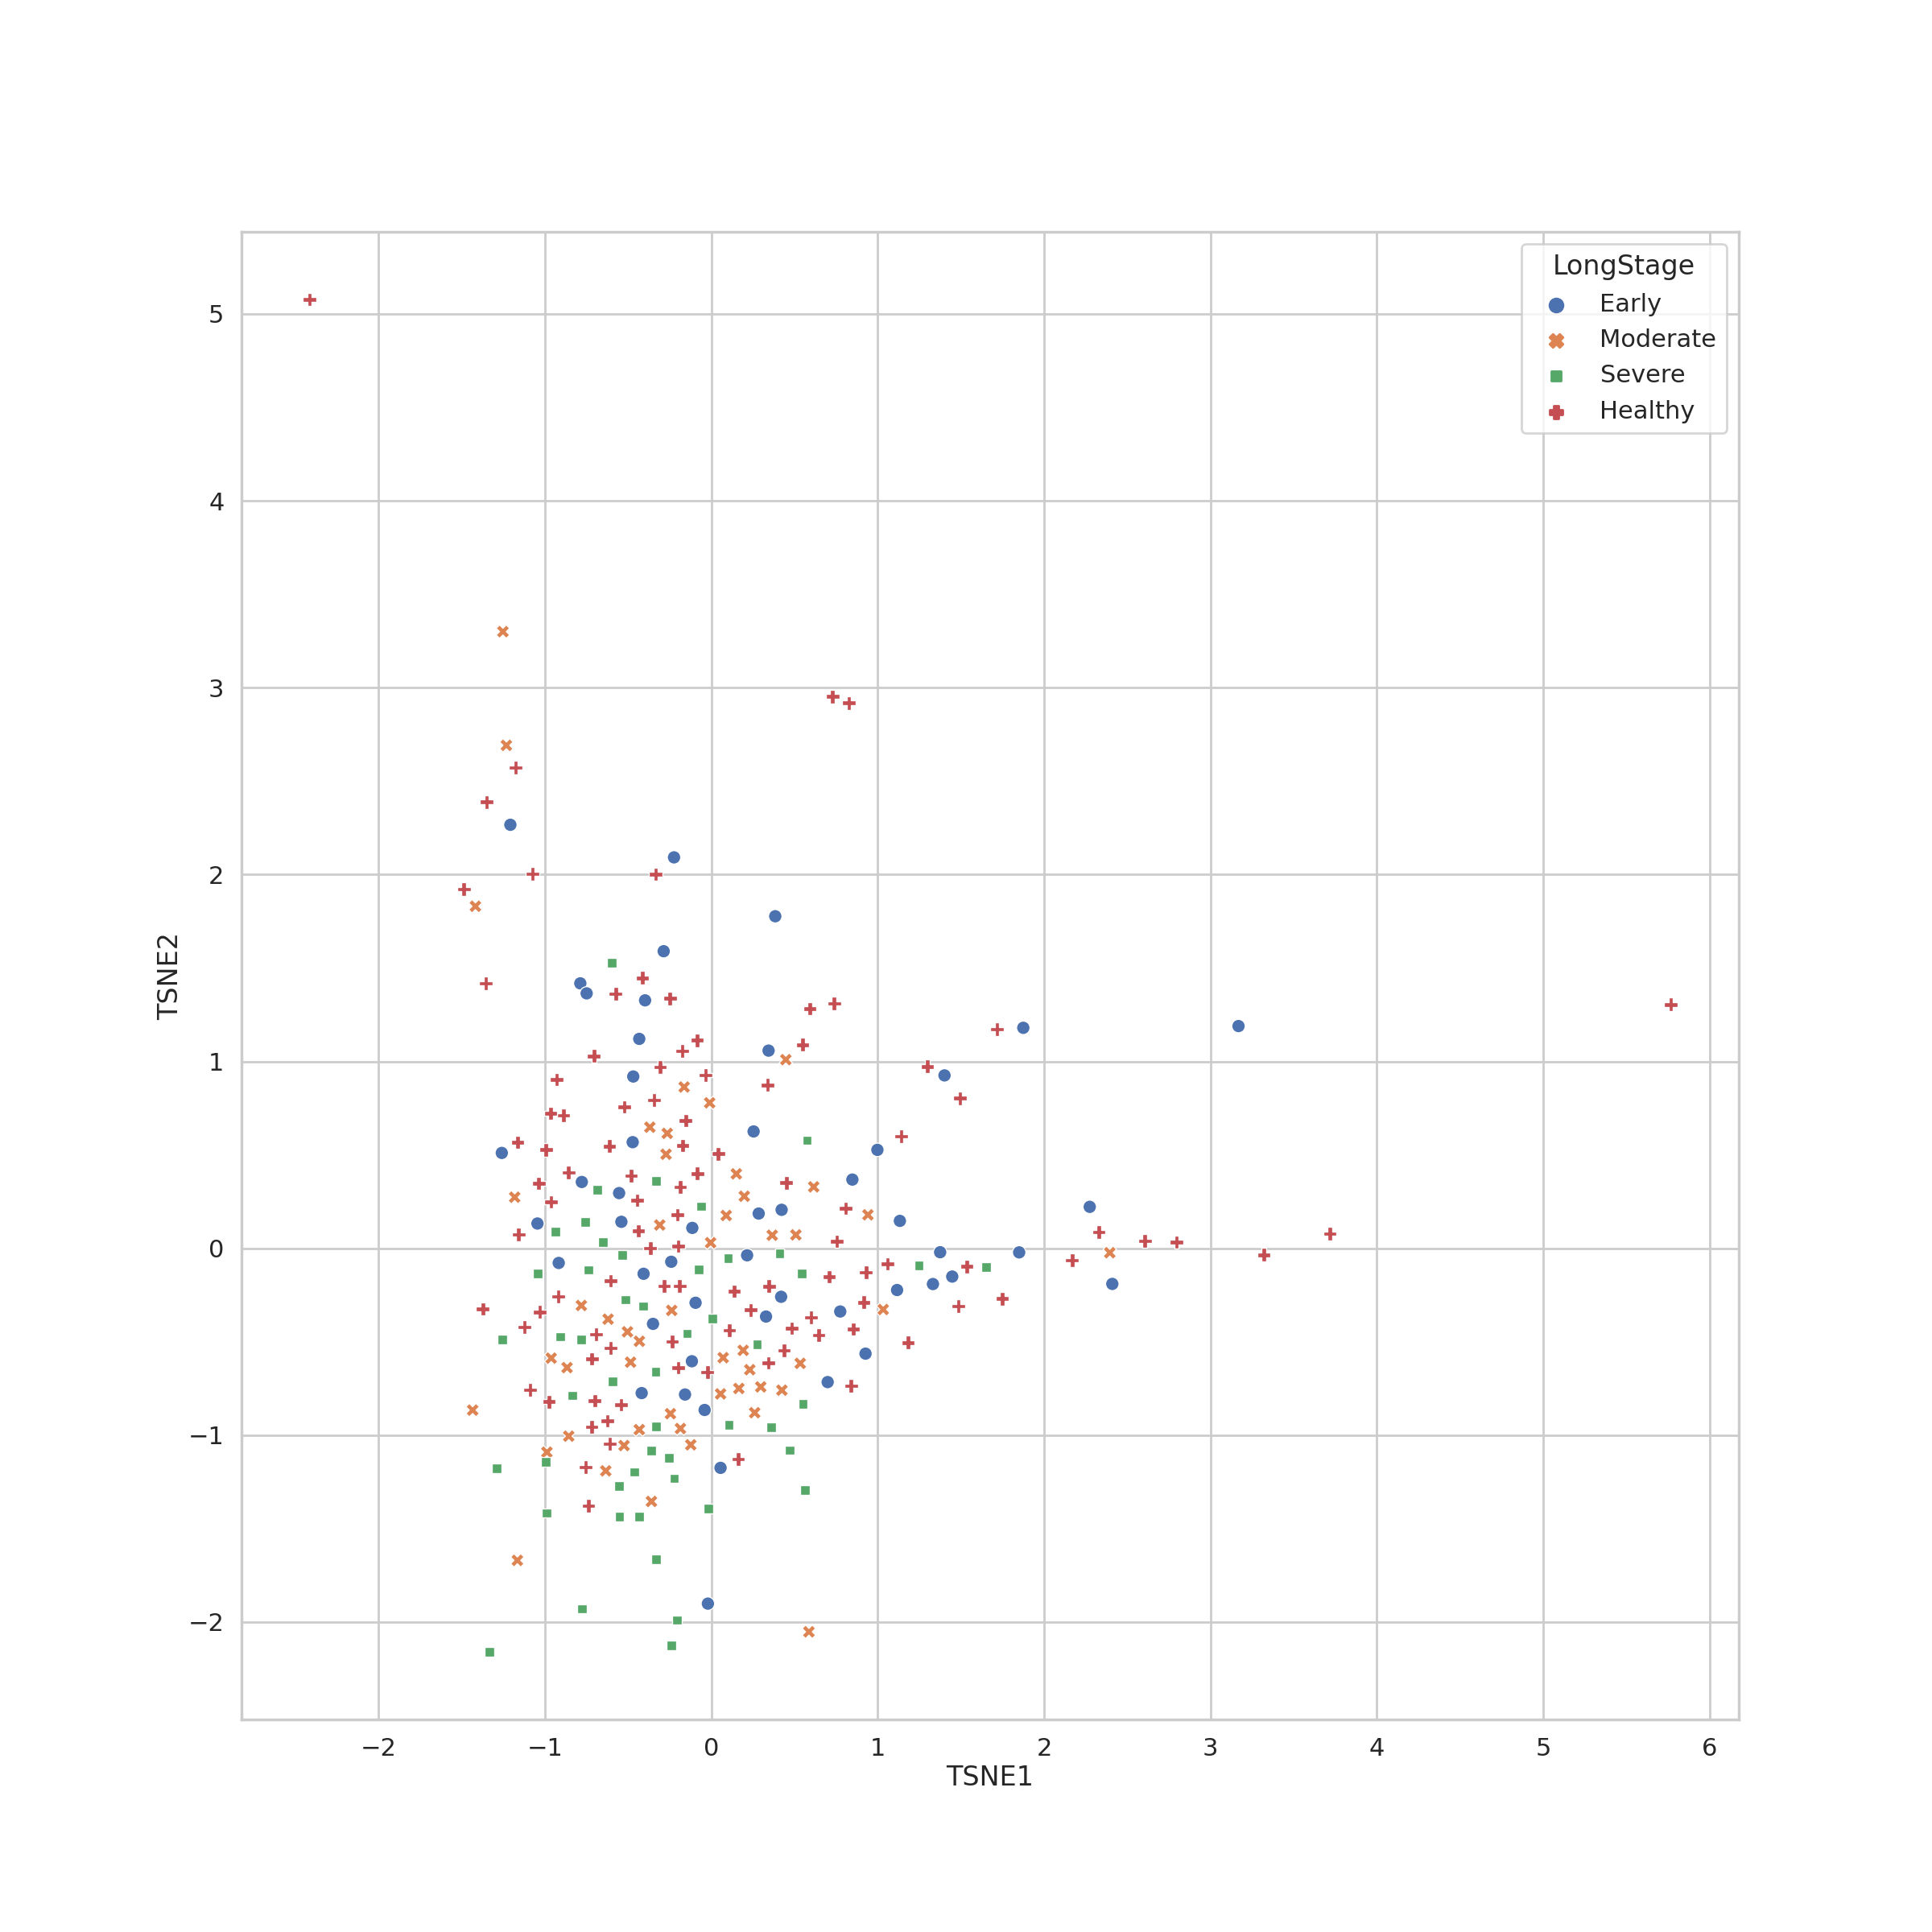
\includegraphics[width=0.6 \linewidth]{figures/tSNE/Whole/whole.Deblur.silva.png}
                \caption{t-SNE Plot with Whole Microbiome from Deblur and SILVA (414 taxa)}
                \label{fig:tsne-whole-deblur-silva}
            \end{figure}

            \begin{figure}[p]
                \centering
                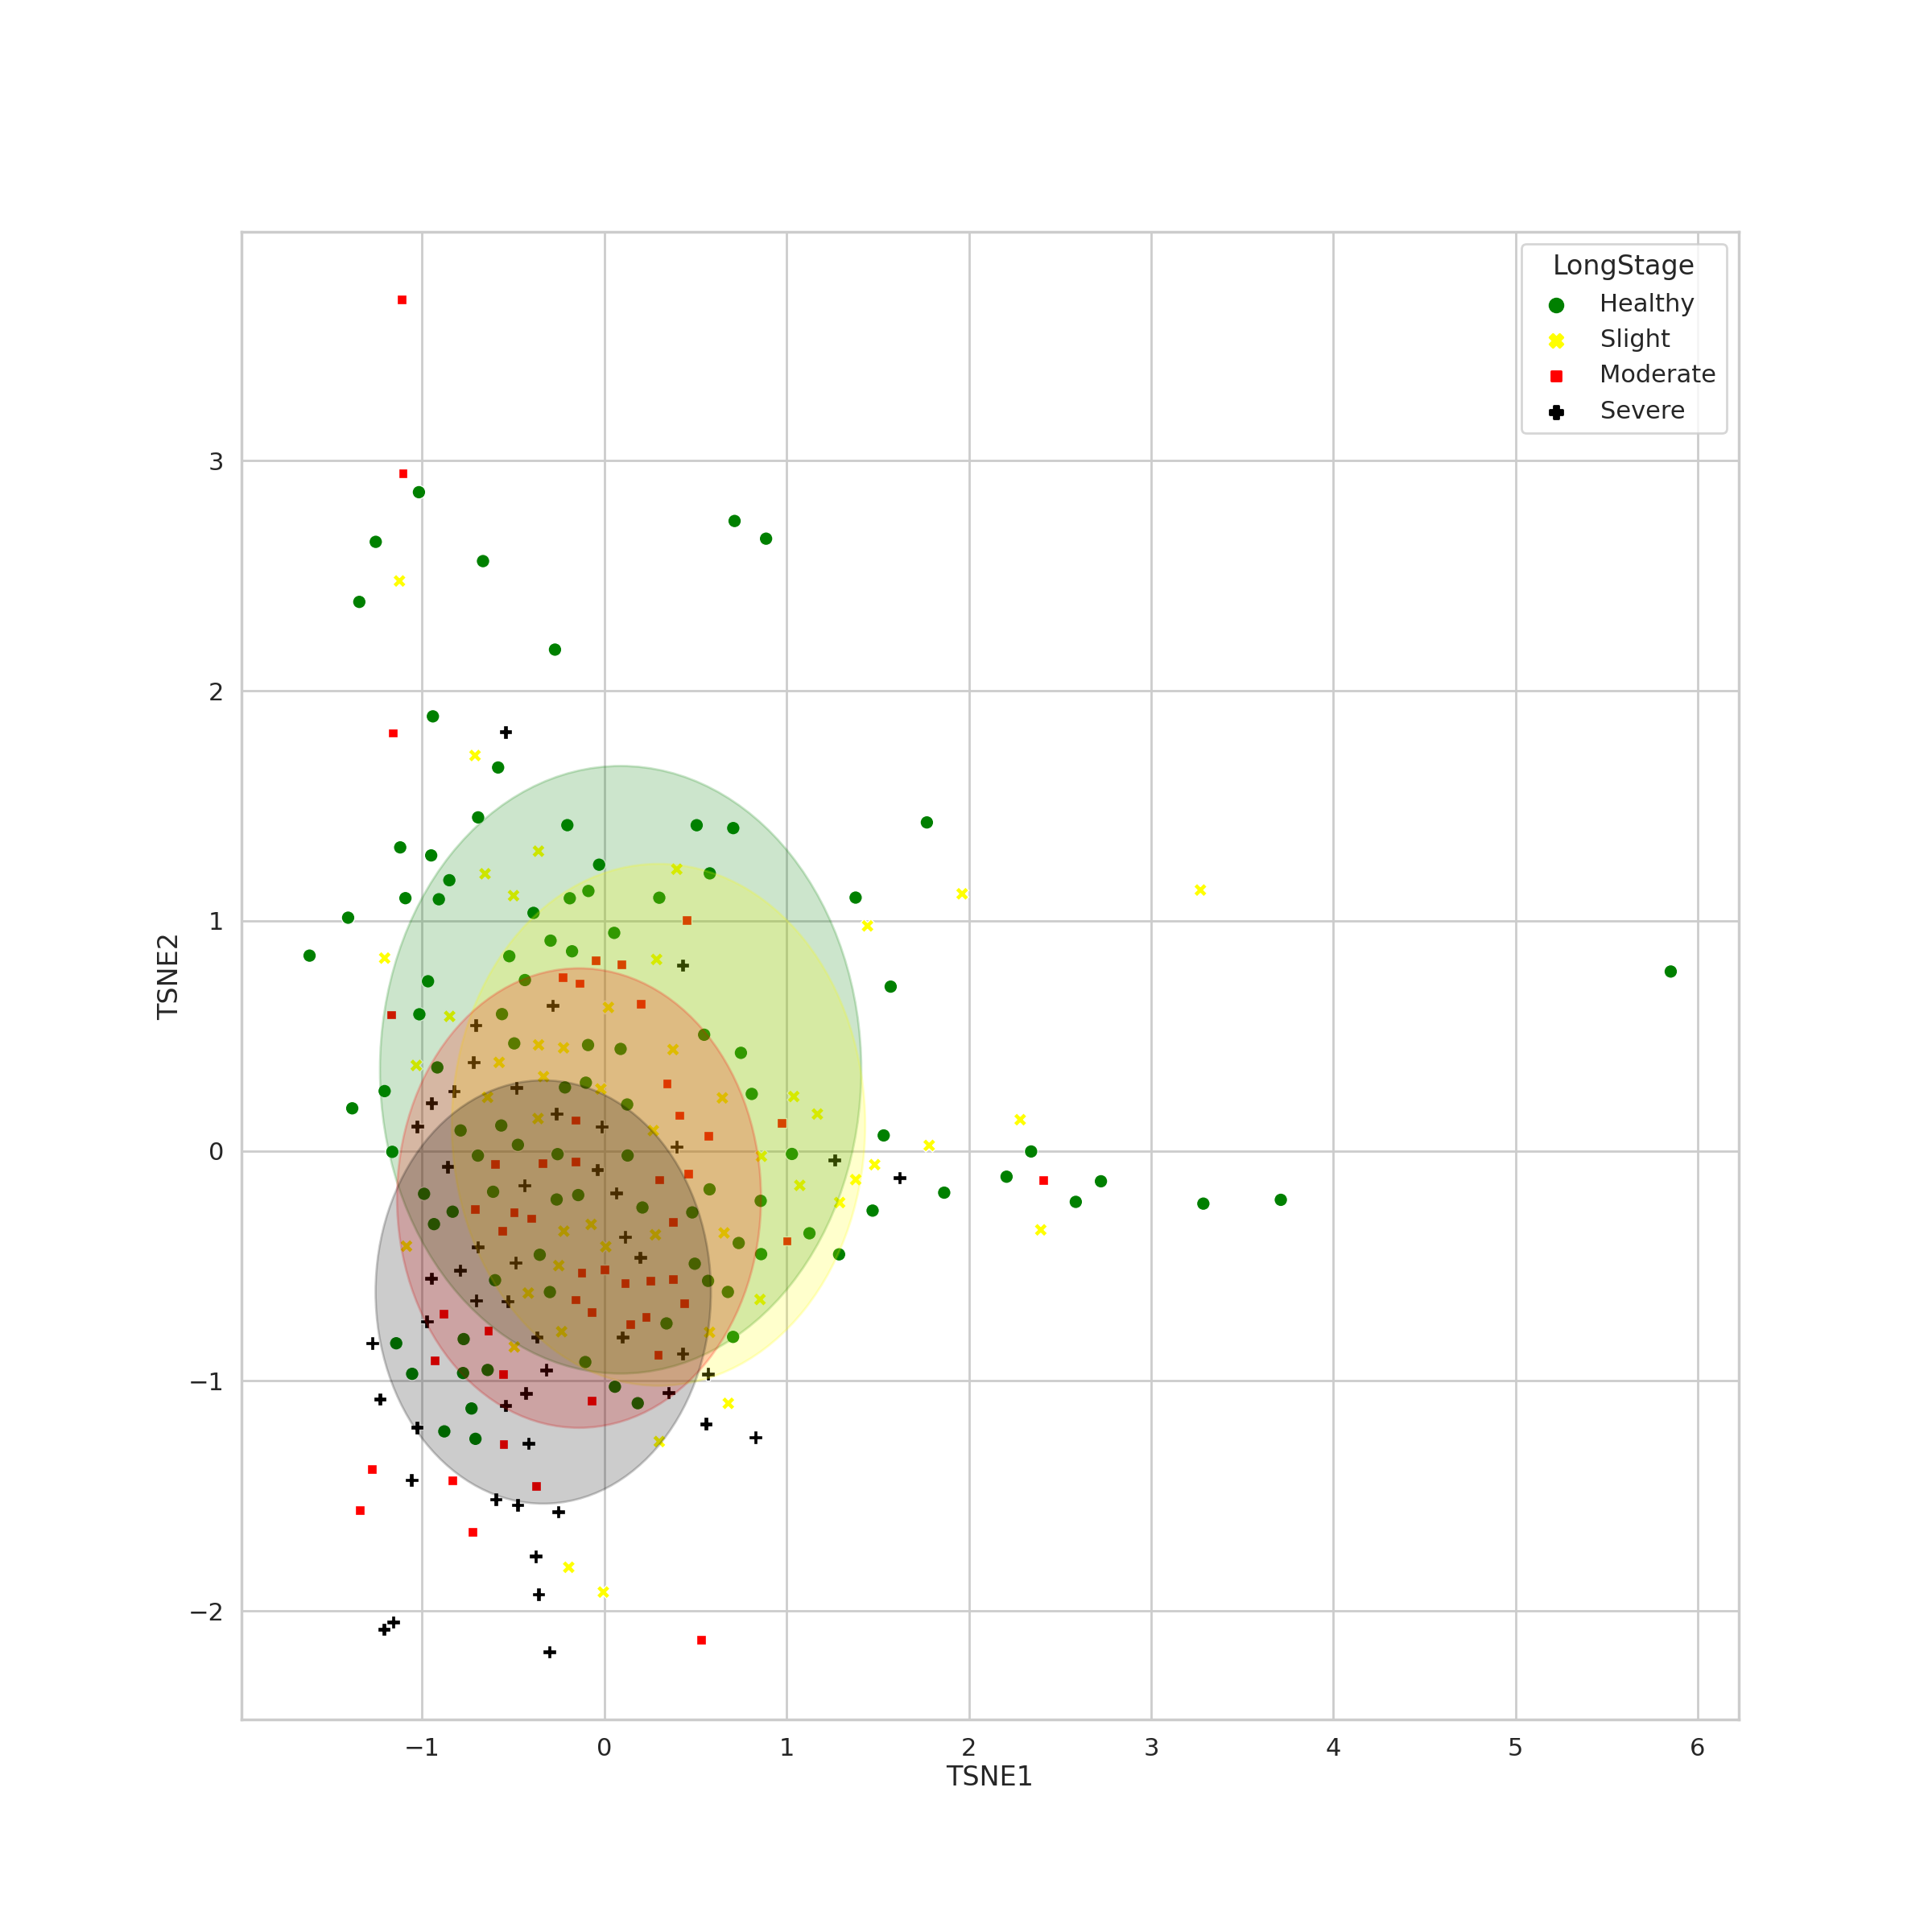
\includegraphics[width=0.6 \linewidth]{figures/tSNE/Whole/whole.Deblur.homd.png}
                \caption{t-SNE Plot with Whole Microbiome from Deblur and HOMD (235 taxa)}
                \label{fig:tsne-whole-deblur-homd}
            \end{figure}

        \subsection{t-SNE Plot with ANCOM Selected Microbiome Data}

            \begin{figure}[p]
                \centering
                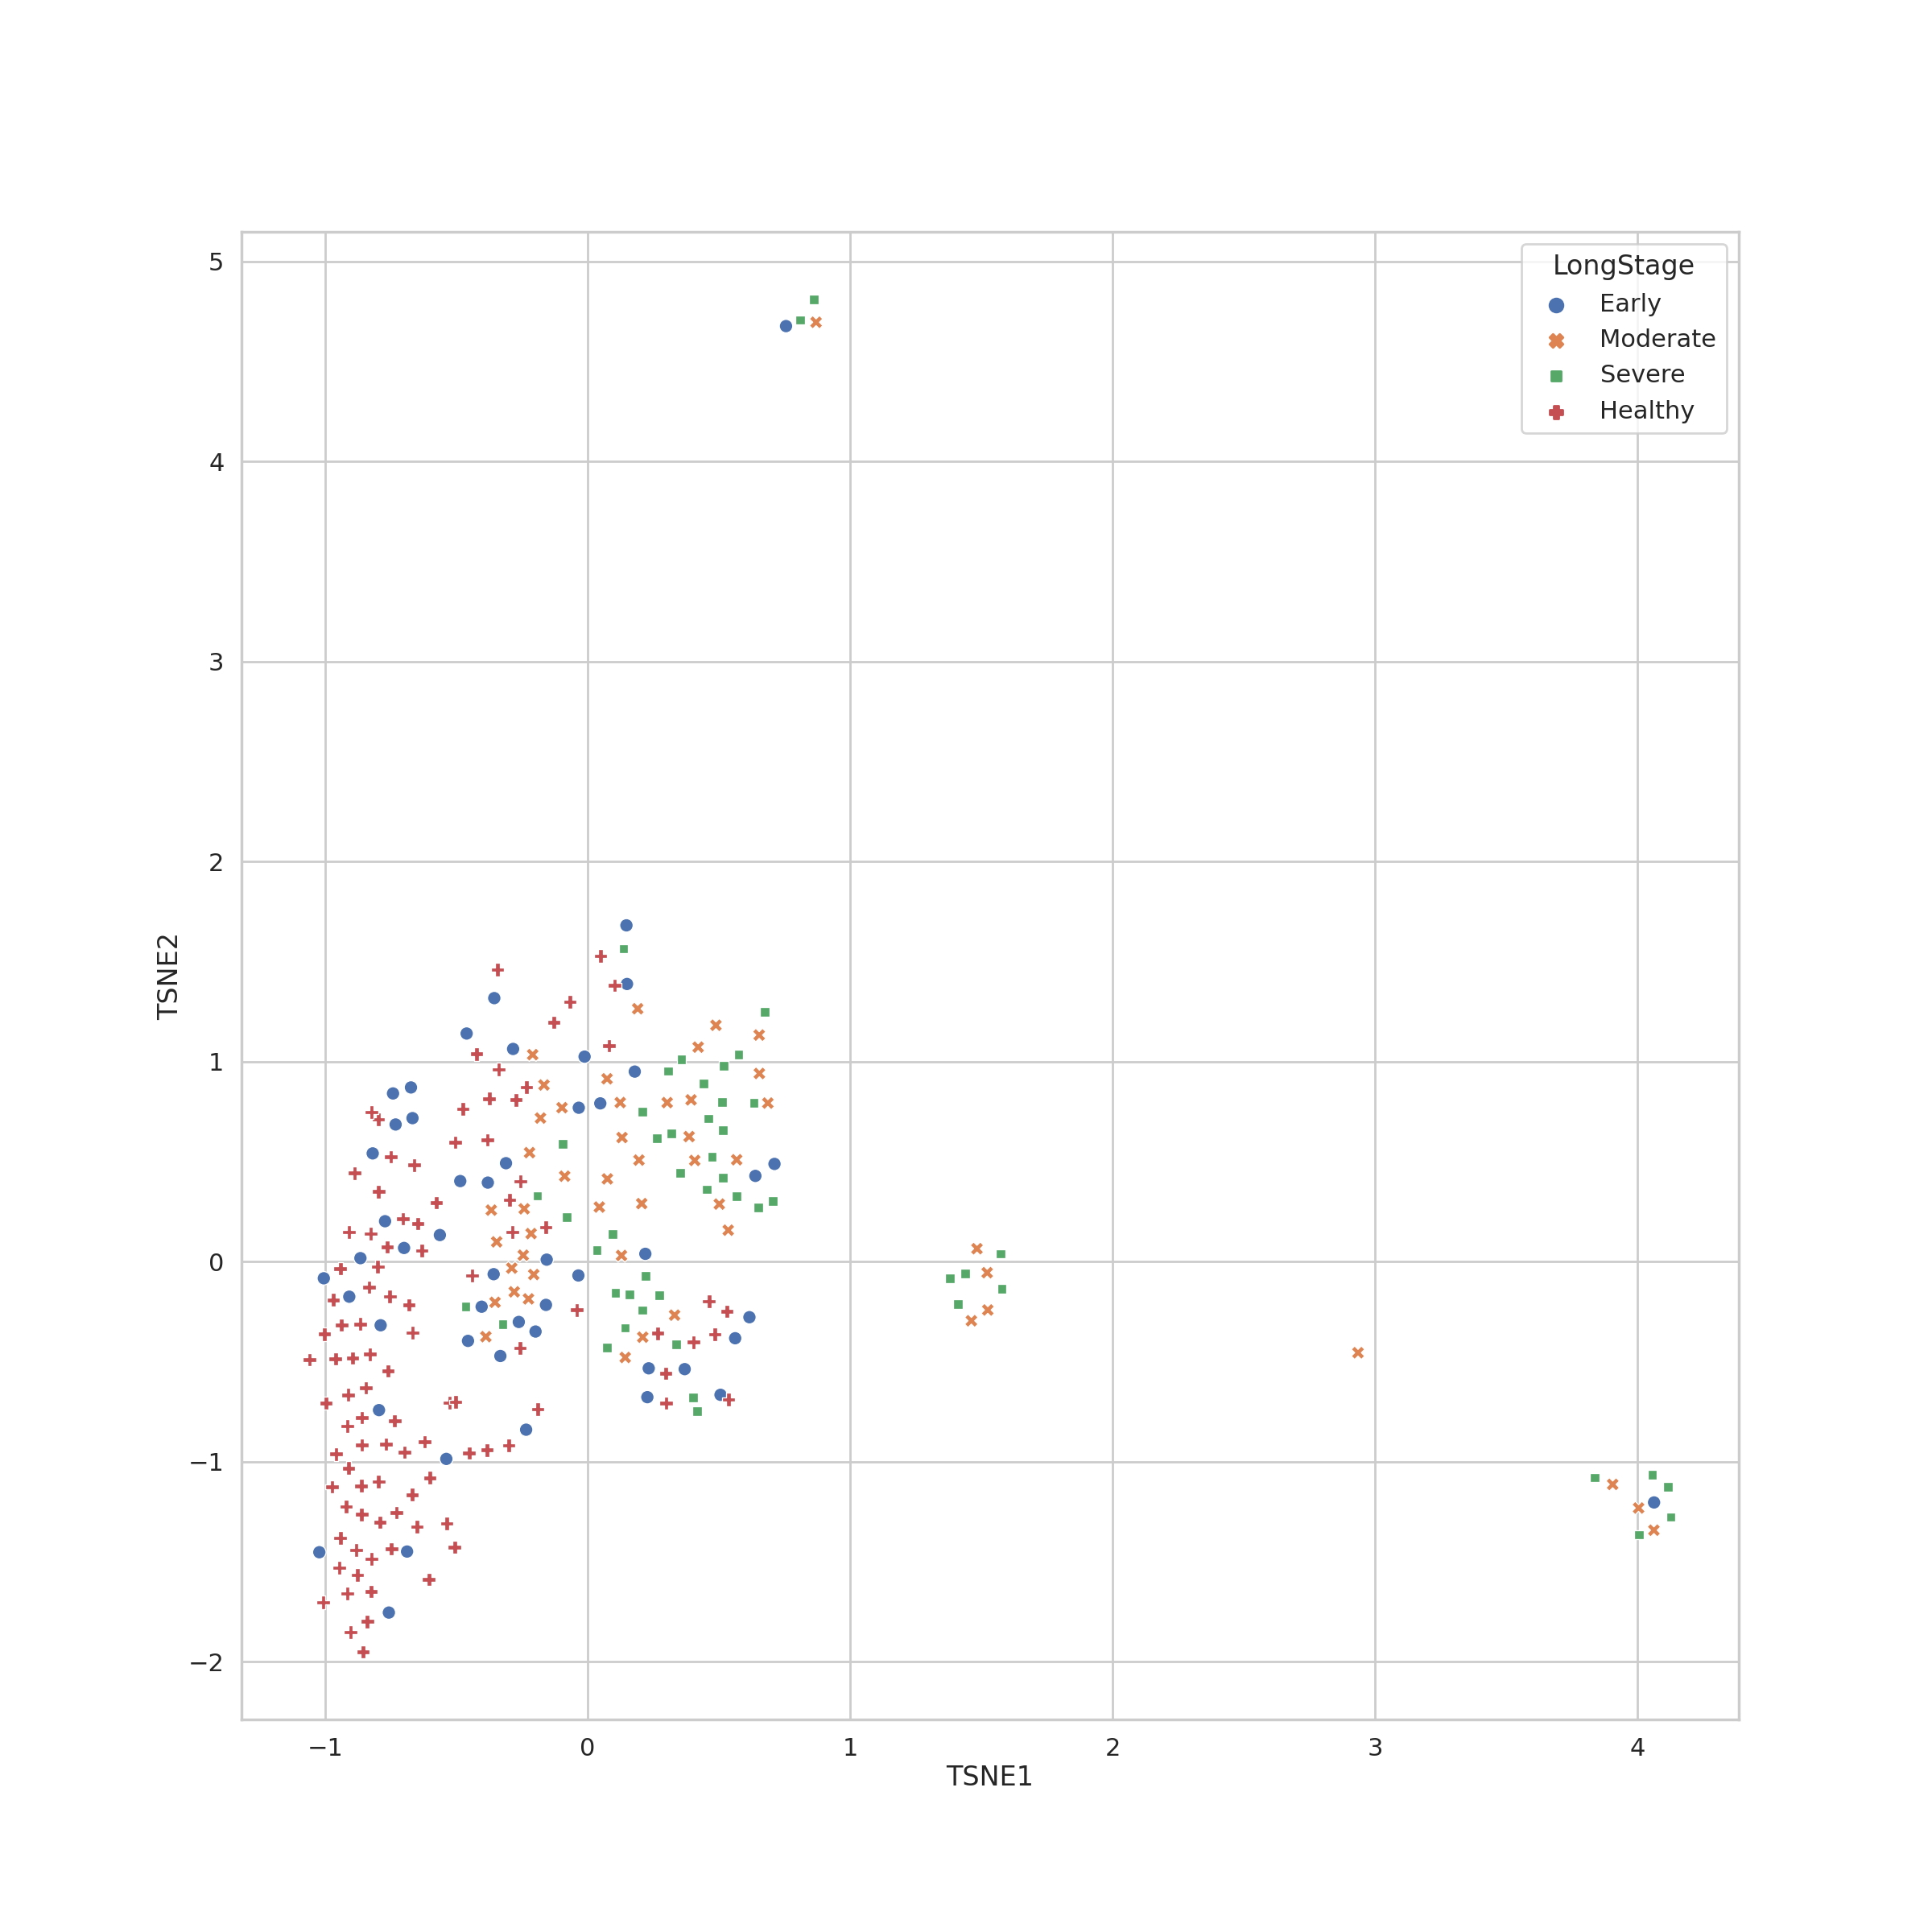
\includegraphics[width=0.6 \linewidth]{figures/tSNE/ANCOM/ANCOM.DADA2.gg.png}
                \caption{t-SNE Plot with ANCOM Selected Microbiome Data from DADA2 and GG (15 taxa)}
                \label{fig:tsne-ANCOM-dada2-gg}
            \end{figure}

            \begin{figure}[p]
                \centering
                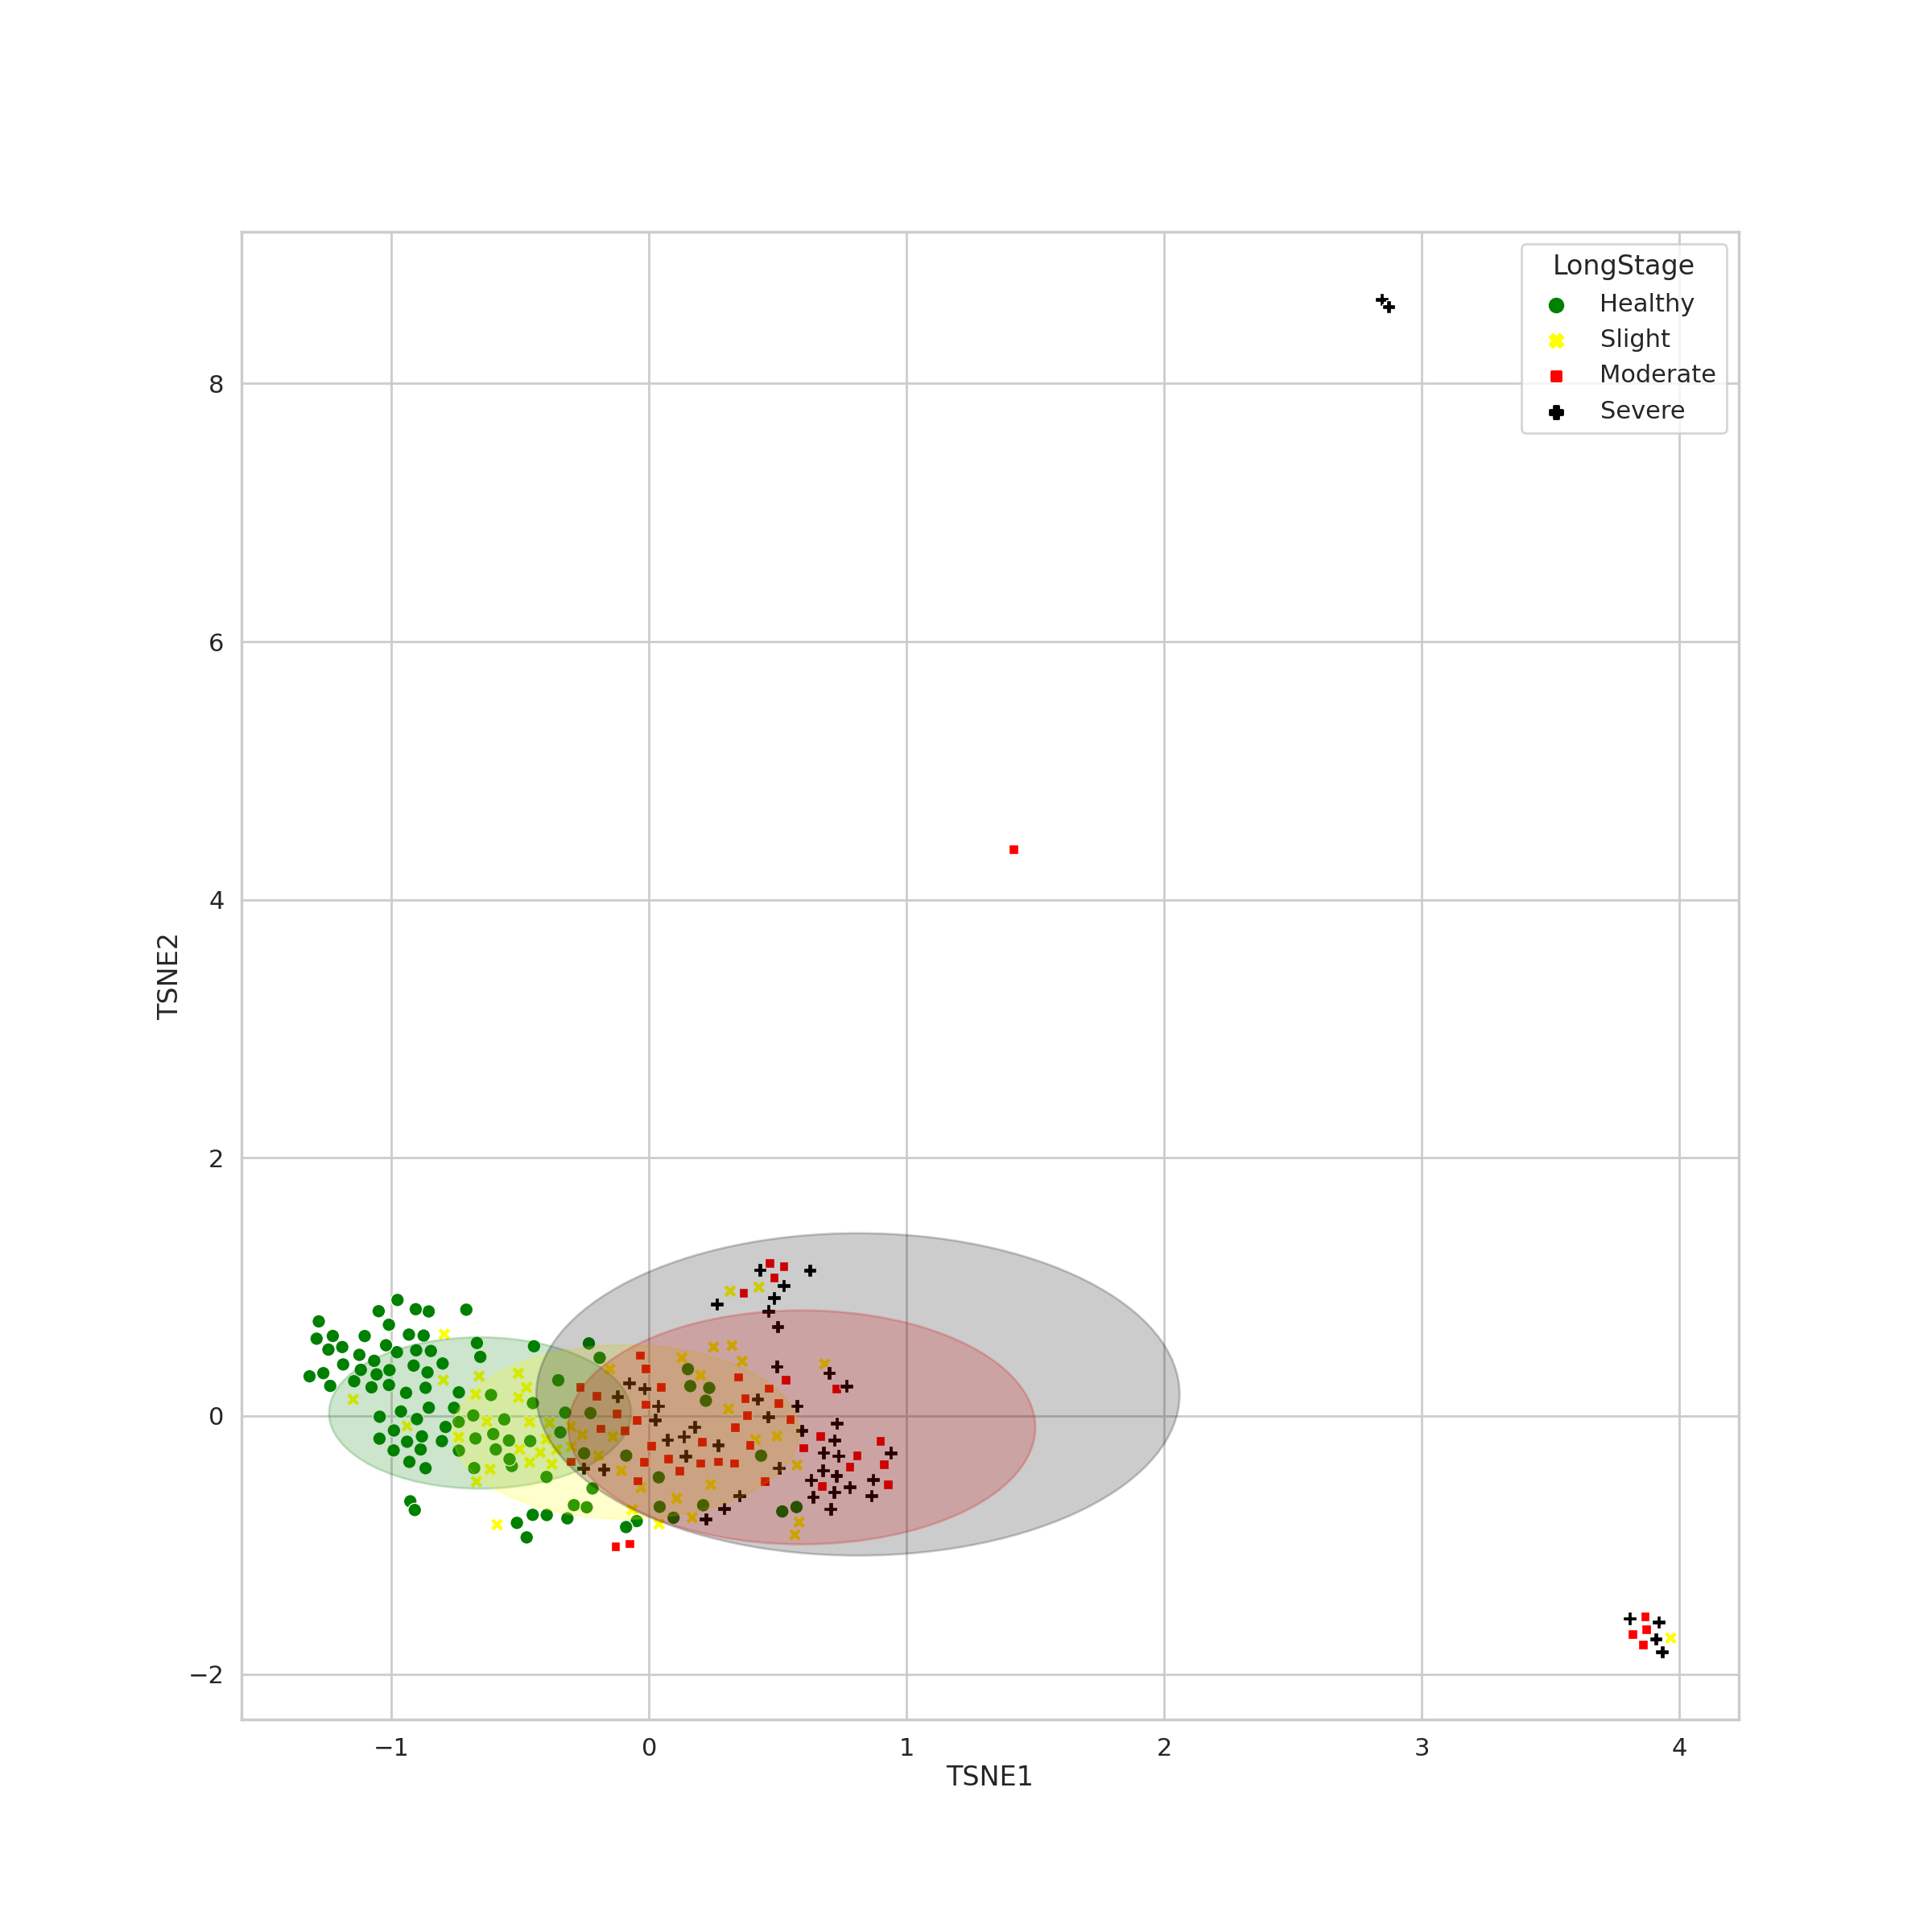
\includegraphics[width=0.6 \linewidth]{figures/tSNE/ANCOM/ANCOM.DADA2.silva.png}
                \caption{t-SNE Plot with ANCOM Selected Microbiome Data from DADA2 and SILVA (23 taxa)}
                \label{fig:tsne-ANCOM-dada2-silva}
            \end{figure}

            \begin{figure}[p]
                \centering
                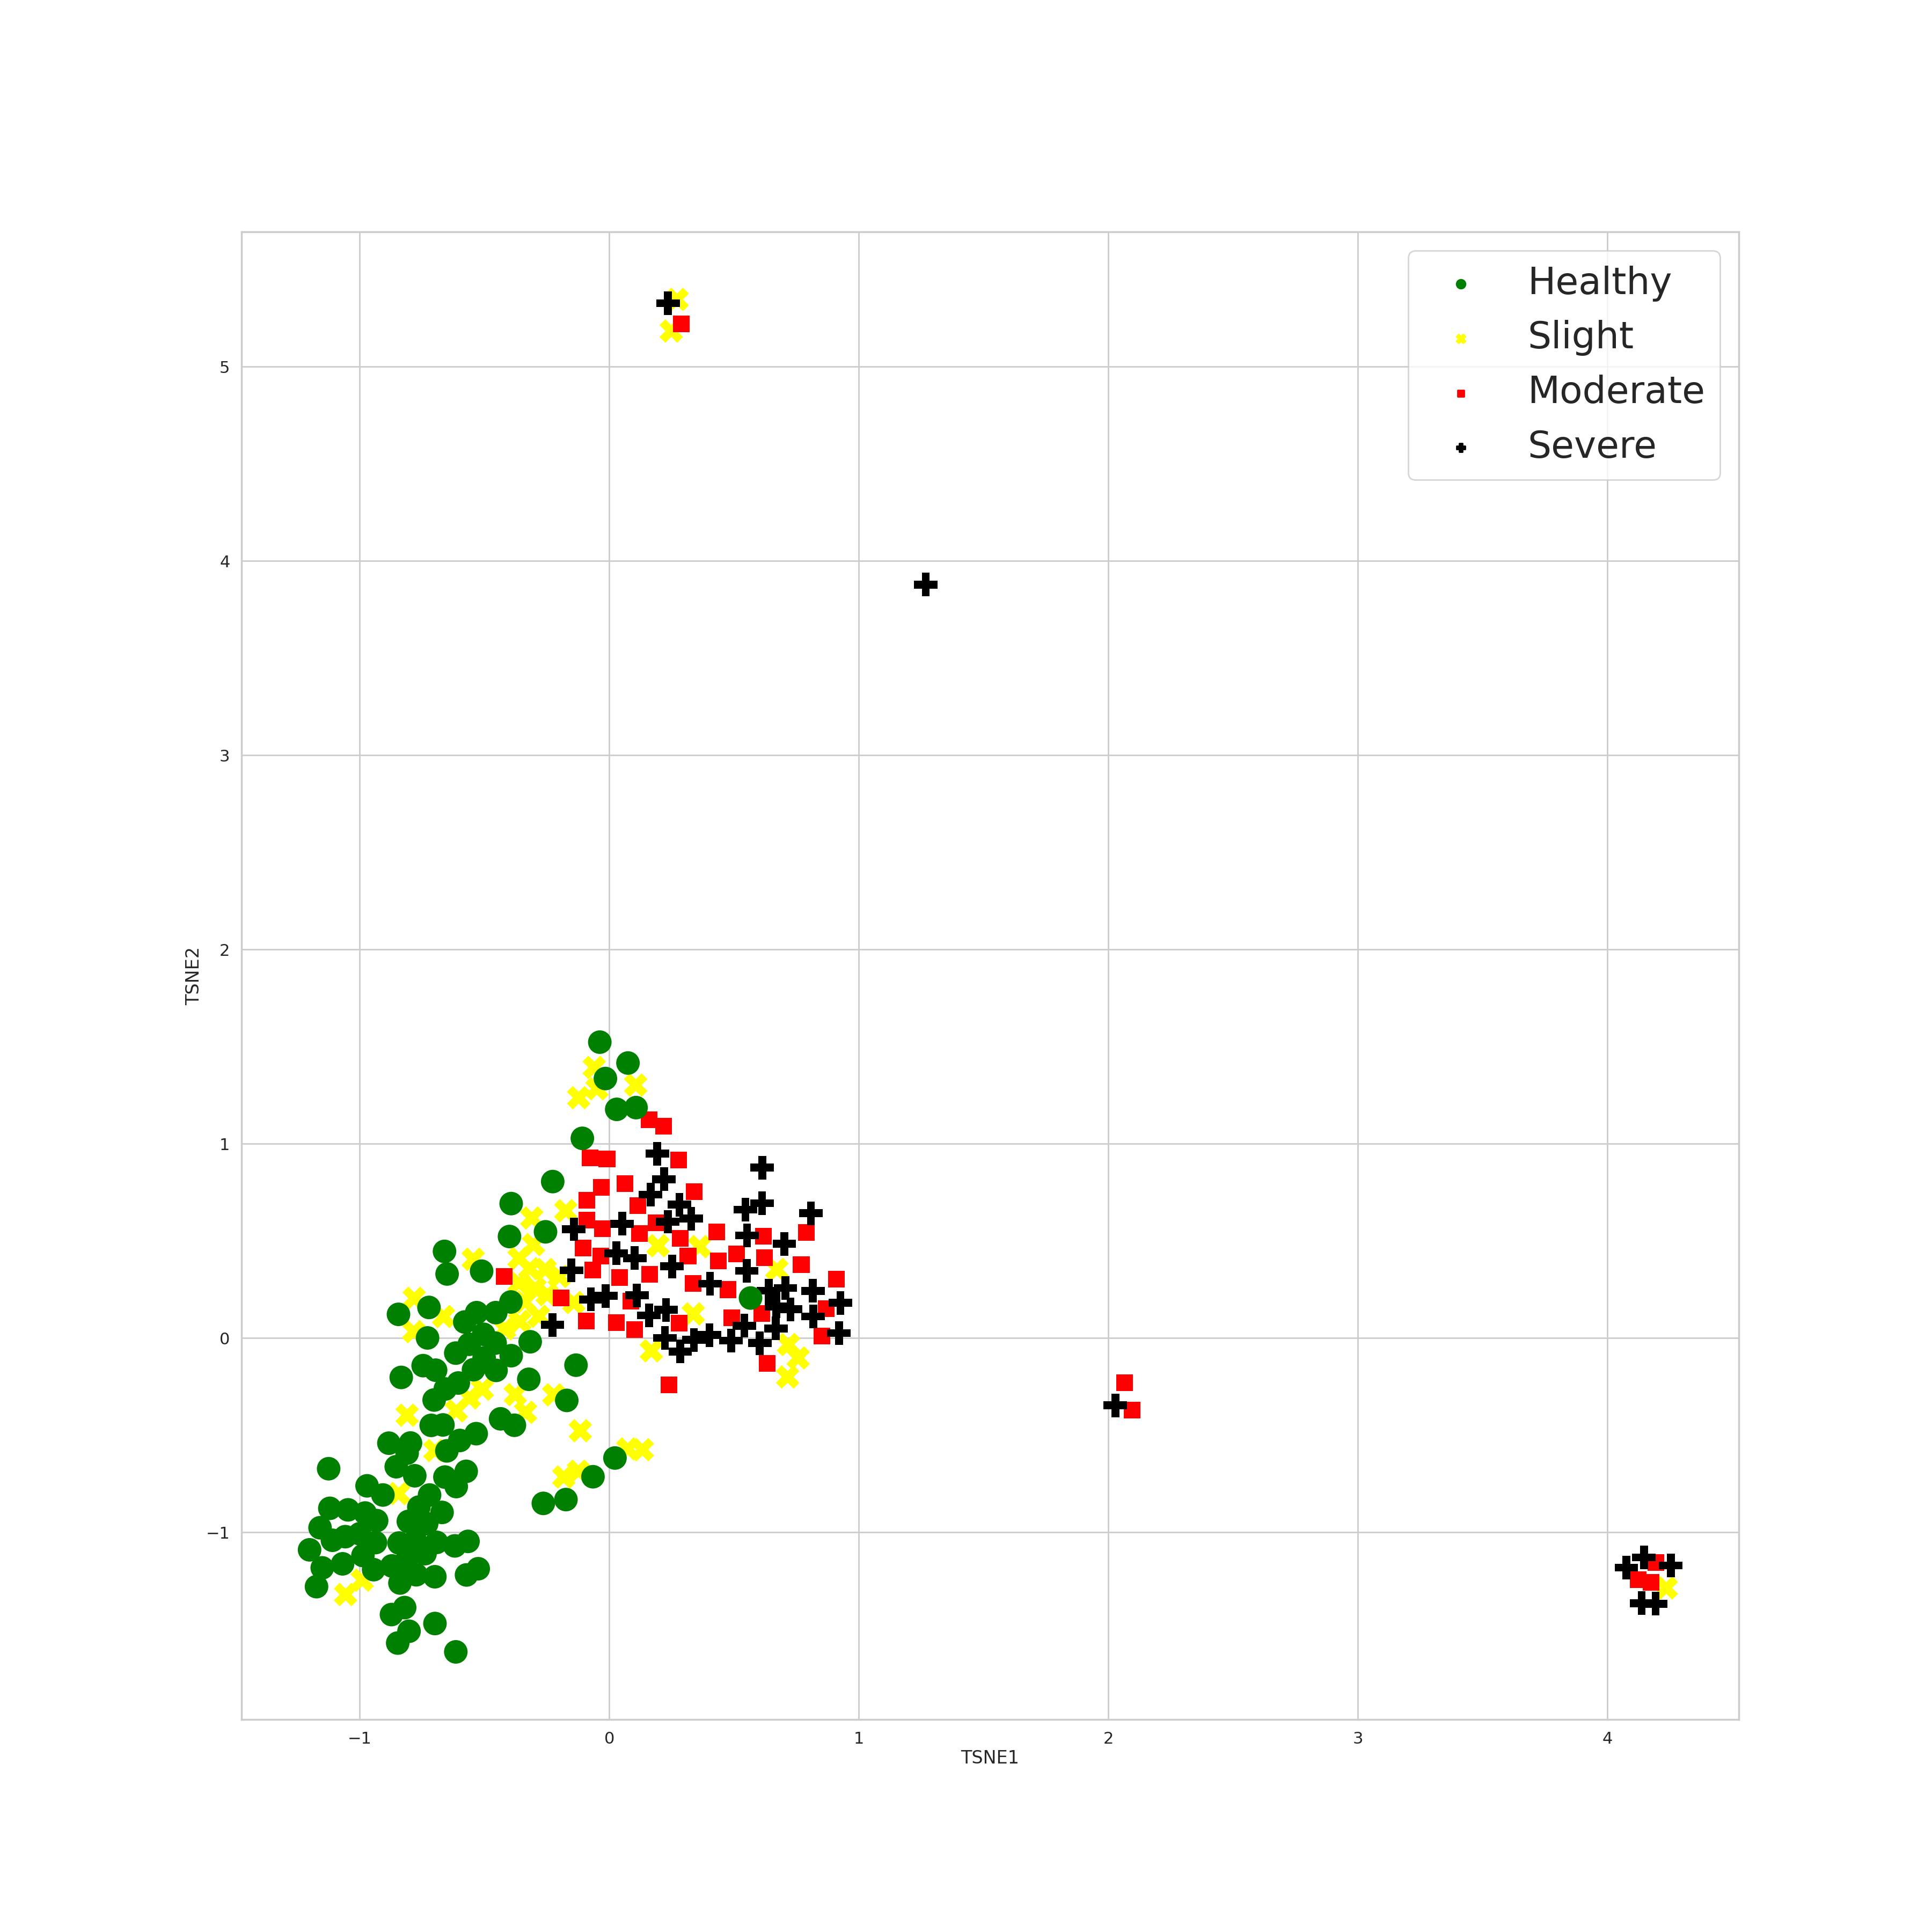
\includegraphics[width=0.6 \linewidth]{figures/tSNE/ANCOM/ANCOM.DADA2.homd.png}
                \caption{t-SNE Plot with ANCOM Selected Microbiome Data from DADA2 and HOMD (20 taxa)}
                \label{fig:tsne-ANCOM-dada2-homd}
            \end{figure}

            \begin{figure}[p]
                \centering
                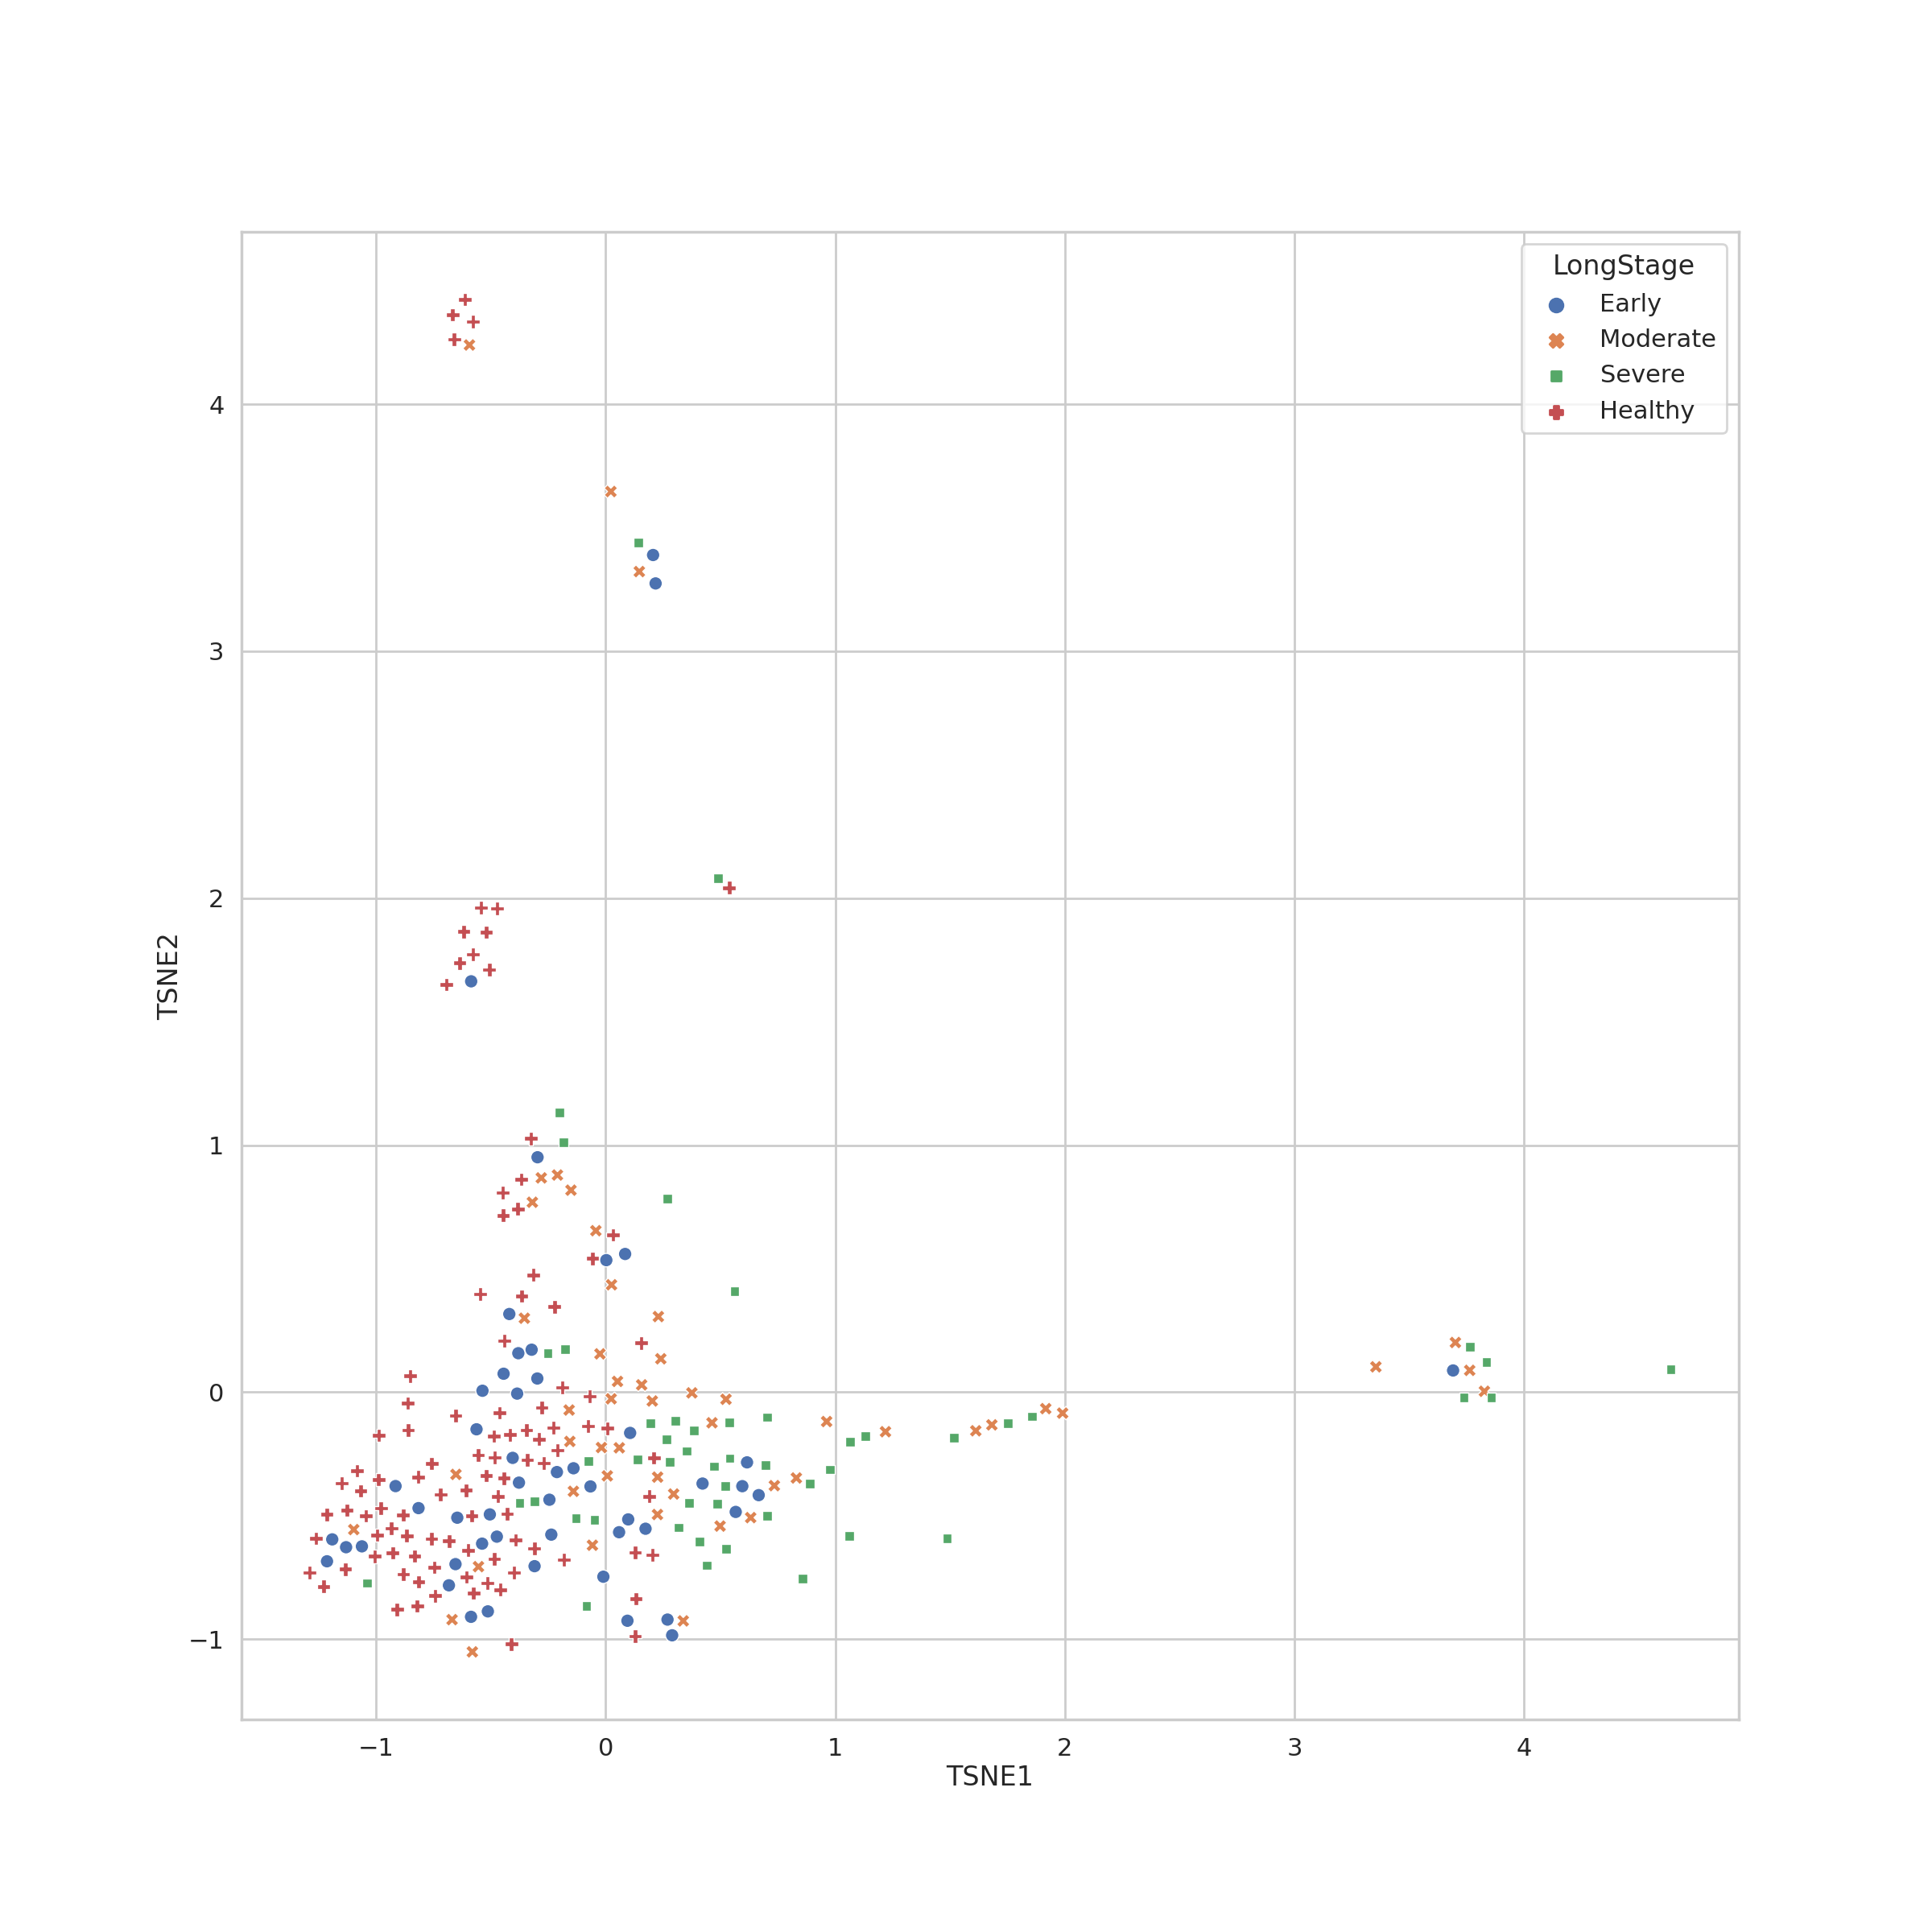
\includegraphics[width=0.6 \linewidth]{figures/tSNE/ANCOM/ANCOM.Deblur.gg.png}
                \caption{t-SNE Plot with ANCOM Selected Microbiome Data from Deblur and GG (27 taxa)}
                \label{fig:tsne-ANCOM-deblur-gg}
            \end{figure}

            \begin{figure}[p]
                \centering
                \includegraphics[width=0.6 \linewidth]{figures/tSNE/ANCOM/ANCOM.Deblur.silva.png}
                \caption{t-SNE Plot with ANCOM Selected Microbiome Data from Deblur and SILVA (20 taxa)}
                \label{fig:tsne-ANCOM-deblur-silva}
            \end{figure}

            \begin{figure}[p]
                \centering
                \includegraphics[width=0.6 \linewidth]{figures/tSNE/ANCOM/ANCOM.Deblur.homd.png}
                \caption{t-SNE Plot with ANCOM Selected Microbiome Data from Deblur and HOMD (28 taxa)}
                \label{fig:tsne-ANCOM-deblur-homd}
            \end{figure}

        \subsection{Random Forest Classifier with Every Class}

            \begin{table}[p]
                \centering
                \caption{Taxa with DADA2 and HOMD Ordered by Random Forest}
                \label{tb:RF-every-DADA2-homd}

                \csvreader[tabular=cp{10cm}l, no head, column count=3, table head=\hline, late after first line=\\\hline, table foot=\hline]{csv/RandomForest/whole-DADA2-homd.csv}{}{\csvlinetotablerow}
            \end{table}

            \begin{figure}[p]
                \centering
                \includegraphics[width=0.7 \linewidth]{figures/RandomForest/ANCOM.DADA2.homd/metrics.png}
                \caption{Metrics by Feature Count with DADA2 and HOMD}
                \label{fig:RF-every-metrics-DADA2-homd}
            \end{figure}

            \begin{figure}[p]
                \centering
                $\begin{array}{cc}
                    \includegraphics[width=0.4 \linewidth]{figures/RandomForest/ANCOM.DADA2.homd/Feature_0.png}
                    &
                    \includegraphics[width=0.4 \linewidth]{figures/RandomForest/ANCOM.DADA2.homd/Feature_1.png}
                    \\
                    \mbox{(a) \textit{Porphyromonas gingivalis}} & \mbox{(b) \textit{Actinomyces}} \\
                \end{array}$
                \caption{Most and Second Most Important Features with DADA2 and HOMD}
                \label{fig:RF-every-important-DADA2-homd}
            \end{figure}

        \subsection{Random Forest Classifier with Merging (Moderate+Severe) Classes}

            \begin{table}[p]
                \centering
                \caption{Taxa with DADA2 and HOMD Ordered by Random Forest for Merging (Moderate+Severe) Classes}
                \label{tb:RF-MS-DADA2-homd}

                \csvreader[tabular=cp{10cm}l, no head, column count=3, table head=\hline, late after first line=\\\hline, table foot=\hline]{csv/RandomForest/two-DADA2-homd.csv}{}{\csvlinetotablerow}
            \end{table}

            \begin{figure}[p]
                \centering
                \includegraphics[width=0.7 \linewidth]{figures/RandomForest/two.DADA2.homd/metrics.png}
                \caption{Metrics by Feature Count with Deblur and HOMD for Merging (Moderate+Severe) Classes}
                \label{fig:RF-MS-metrics-DADA2-homd}
            \end{figure}

            \begin{figure}[p]
                \centering
                $\begin{array}{cc}
                    \includegraphics[width=0.4 \linewidth]{figures/RandomForest/two.DADA2.homd/Feature_0.png}
                    &
                    \includegraphics[width=0.4 \linewidth]{figures/RandomForest/two.DADA2.homd/Feature_1.png}
                    \\
                    \mbox{(a) \textit{Porphyromonas gingivalis}} & \mbox{(b) \textit{Actinomyces}} \\
                \end{array}$
                \caption{Most and Second Most Important Features with Deblur and HOMD for Merging (Moderate+Severe) Classes}
                \label{fig:RF-MS-important-DADA2-homd}
            \end{figure}

        \subsection{Random Forest Classifier with Healthy Class and Early Class Only}

            \begin{table}[p]
                \centering
                \caption{Taxa with DADA2 and HOMD Ordered by Random Forest for Healthy Class and Early Class Only}
                \label{tb:RF-HEonly-DADA2-homd}

                \csvreader[tabular=cp{10cm}l, no head, column count=3, table head=\hline, late after first line=\\\hline, table foot=\hline]{csv/RandomForest/HE-DADA2-homd.csv}{}{\csvlinetotablerow}
            \end{table}

            \begin{figure}[p]
                \centering
                \includegraphics[width=0.7 \linewidth]{figures/RandomForest/HE.DADA2.homd/metrics.png}
                \caption{Metrics by Feature Count with DADA2 and HOMD for Healthy Class and Early Class Only}
                \label{fig:RF-HEonly-metrics-DADA2-homd}
            \end{figure}

            \begin{figure}[p]
                \centering
                $\begin{array}{cc}
                    \includegraphics[width=0.4 \linewidth]{figures/RandomForest/HE.DADA2.homd/Feature_0.png}
                    &
                    \includegraphics[width=0.4 \linewidth]{figures/RandomForest/HE.DADA2.homd/Feature_1.png}
                    \\
                    \mbox{(a) \textit{Porphyromonas gingivalis}} & \mbox{(b) \textit{Treponema denticola}} \\
                \end{array}$
                \caption{Most and Second Most Important Features with DADA2 and HOMD for Healthy Class and Early Class Only}
                \label{fig:RF-HEonly-important-DADA2-homd}
            \end{figure}

    \section{Discussion}
        \subsection{Alpha-diversity}
            Alpha-diversity indices among all groups from DADA2 are in table \ref{tb:alpha-all-dada2}. Shannon's diversity index in DADA2, though, has marginally significant p-value; the other indices have strongly significant p-values. Additionally, there are no statistically significant differences between (Healthy and Early) classes and (Moderate and Severe) classes with evenness index from DADA2 (Table \ref{tb:alpha-evenness-dada2} and Figure \ref{fig:evenness-dada2}). Also, there is no statistically significant difference between (Healthy and Early) classes with Faith's phylogenetic diversity index from DADA2 (Table \ref{tb:alpha-faith-dada2} and Figure \ref{fig:faith-dada2}). Moreover, there are no statistically significant differences between (Early and Moderate) classes, (Early and Severe) classes and (Moderate and Severe) classes with observed feature index from DADA2 (Table \ref{tb:alpha-observed-dada2} and Figure \ref{fig:observed-dada2}). Furthermore, there are no statistically significant differences between (Healthy and Moderate) classes, (Healthy and Severe) classes, (Early and Moderate) classes and (Moderate and Severe) classes from Shannon's diversity index from DADA2 (Table \ref{tb:alpha-shannon-dada2} and Figure \ref{fig:shannon-dada2}).

            Alpha-diversity indices among all groups from Deblur are in table \ref{tb:alpha-all-deblur}. Every index have strongly significant p-values. Additionally, there are no statistically significant differences between (Healthy and Early) classes, (Healthy and Moderate) classes, (Healthy and Severe) classes and (Moderate and Severe) classes with evenness index from Deblur (Table \ref{tb:alpha-evenness-deblur} and Figure \ref{fig:evenness-deblur}). Also, there are no statistically significant differences between (Healthy and Early) classes and (Moderate and Severe) classes with Faith's phylogenetic diversity index from Deblur (Table \ref{tb:alpha-faith-deblur} and Figure \ref{fig:faith-deblur}). Moreover, there are no statistically significant differences between (Healthy and Early) classes and (Moderate and Severe) classes with observed features index from Deblur (Table \ref{tb:alpha-observed-deblur} and Figure \ref{fig:observed-deblur}). Furthermore, there are no statistically significant differences between (Healthy and Early) classes and (Moderate and Severe) classes with Shannon's diversity index from Deblur (Table \ref{tb:alpha-shannon-deblur} and Figure \ref{fig:shannon-deblur}).

            Merging similar classes could elevate classification metrics; while merging must result mere primitive classification than without merging classes. Accordingly, deciding merged classes should be rigorous and resolutely reasoned. In result, many pairs of classes should be merged as value of alpha-diversity indices, for instance (Healthy and Early) classes, (Healthy and Severe) classes and (Moderate and Severe) classes. Despite alpha-diversity indices show no significant differences, some pairs of classes have to refuse to be merged in two major reasons. First, merging those classes is fallacious. For example, (Healthy and Severe) classes, without loss of generality. Healthy class and Severe class does not adjoin each other, in terms of clinical stage. Second, even those classes are adjacent each other, some pairs of classes have not enough results to merge. For instance, null hypothesis from (Early and Moderate) classes is only sustained by Shannon's diversity index (Table \ref{tb:alpha-shannon-dada2}), so merging Early class and Moderate class cannot be reasoned. Hence, two pairs of classes will be merged in classification: (Healthy and Early) classes and (Moderate and Severe) classes.

        \subsection{Beta-diversity}
            From data with DADA2, all beta-diversity distance index, includes Bray-Curtis distance index (Table \ref{tb:bray-dada2}, Figure \ref{fig:tsne-bray-dada2} and Figure \ref{fig:bray-dada2}), Jaccard distance index (Table \ref{tb:jaccard-dada2}, Figure \ref{fig:tsne-jaccard-dada2} and Figure \ref{fig:jaccard-dada2}), unweighted UniFrac distance index (Table \ref{tb:unweighted-dada2}, Figure \ref{fig:tsne-unweighted-dada2} and Figure \ref{fig:unweighted-dada2}) and weighted UniFrac distance index (Table \ref{tb:weighted-dada2}, Figure \ref{fig:tsne-weighted-dada2} and Figure \ref{fig:weighted-dada2}), show statistically significant differences in every pair of classes, except (Moderate and Severe) classes.

            Bray-Curtis distance index with Deblur has no statistically significant differences between (Healthy and Early) classes and (Moderate and Severe) classes (Table \ref{tb:bray-deblur}, Figure \ref{fig:tsne-bray-deblur} and Figure \ref{fig:bray-deblur}). Moreover, Jaccard distance index with Deblur has no statistically significant difference between (Moderate and Severe) classes (Table \ref{tb:jaccard-deblur}, Figure \ref{fig:tsne-jaccard-deblur} and Figure \ref{fig:jaccard-deblur}). Additionally, unweighted UniFrac distance index with Deblur has no statistically significant difference between (Moderate and Severe) classes (Table \ref{tb:unweighted-deblur}, Figure \ref{fig:tsne-unweighted-deblur} and Figure \ref{fig:unweighted-deblur}). Furthermore, weighted UniFrac distance index with Deblur has no statistically significant difference between (Healthy and Early) classes (Table \ref{fig:weighted-deblur}, Figure \ref{fig:tsne-weighted-deblur} and Figure \ref{fig:weighted-deblur}).

            As results of alpha-diversity indices, (Healthy and Early) classes and (Moderate and Severe) classes will be merged. Mercifully, alternative fact does totally not sustained by beta-divesity indices. Hence, (Healthy and Early) classes and (Moderate and Severe) classes, as mentioned herein-before, will be merged in classification.

        \subsection{t-SNE Plot}
            Overall distribution of taxa from each sample can be realized by t-SNE plot. If each class is evenly distributed on t-SNE plot, then the data might be difficult for classifying. In this manner, t-SNE plots with whole microbiome (Figure \ref{fig:tsne-whole-dada2-gg}, Figure \ref{fig:tsne-whole-dada2-silva}, Figure \ref{fig:tsne-whole-dada2-homd}, Figure \ref{fig:tsne-whole-deblur-gg}, Figure \ref{fig:tsne-whole-deblur-silva} and Figure \ref{fig:tsne-whole-deblur-homd}) are more evenly distributed, whereas t-SNE plots with ANCOM selected microbiome data (Figure \ref{fig:tsne-ANCOM-dada2-gg}, Figure \ref{fig:tsne-ANCOM-dada2-silva}, Figure \ref{fig:tsne-ANCOM-dada2-homd}, Figure \ref{fig:tsne-ANCOM-deblur-gg}, Figure \ref{fig:tsne-ANCOM-deblur-silva} and Figure \ref{fig:tsne-ANCOM-deblur-homd}) are biased by classes. \textit{Id est}, data with ANCOM selected microbiome could result better in classifying. Hence, ANCOM selected taxa will be used in classification.

        \subsection{Random Forest Classifier}
            As results of Random Forest classifier, a feature or two features have dominant importance than others (Table \ref{tb:RF-every-Deblur-homd}, Table \ref{tb:RF-HE-DADA2-homd}, Table \ref{tb:RF-MS-Deblur-homd}, Table \ref{tb:RF-HEMS-DADA2-silva} and Table \ref{tb:RF-HEonly-DADA2-homd}). Thus, the two most important features are displayed for results of Random Forest classifier (Figure \ref{fig:RF-every-important-Deblur-homd}, Figure \ref{fig:RF-HE-important-DADA2-homd}, Figure \ref{fig:RF-MS-important-Deblur-homd}, Figure \ref{fig:RF-HEMS-important-DADA2-silva} and Figure \ref{fig:RF-HEonly-important-DADA2-homd}).

    \bibliographystyle{apacite}
    \bibliography{reference}
\end{document}